% This is part of Exercices et corrigés de CdI-1
% Copyright (c) 2011
%   Laurent Claessens
% See the file fdl-1.3.txt for copying conditions.

% This is part of Exercices et corrigés de CdI-1
% Copyright (c) 2011
%   Laurent Claessens
% See the file fdl-1.3.txt for copying conditions.

\documentclass[a4paper,12pt]{book}
%\documentclass[a4paper,12pt,draft]{book}

\usepackage{latexsym}
\usepackage{amsfonts}
\usepackage{amsmath}
\usepackage{amsthm}
\usepackage{amssymb}
\usepackage{bbm}
\usepackage{cases}

\usepackage{lscape}

%\usepackage[notcite,notref]{showkeys}

%\usepackage{eso-pic}
%\usepackage{pstricks}
%\usepackage{pst-node}
%\usepackage{pst-eucl}
%\usepackage{pst-abspos}
%\usepackage{pst-plot}
%\usepackage{pst-math}
%\usepackage{pstricks-add}
%\usepackage{subfigure}


\usepackage{pstricks,pst-eucl,pstricks-add,calc,subfigure}		% For phystricks


\usepackage{multido}
\usepackage{fp}
\usepackage{ifthen}
\usepackage{graphicx}

\usepackage{makeidx}
\usepackage{isotope}
\usepackage[cdot,thinqspace,amssymb]{SIunits} 
 % L'option amssymb sert à éviter un conflit avec la commande \square de amssymb. Note qu'elle n'est plus accessible. Si tu en as besoin, faudra RTFM
%ftp://ftp.belnet.be/packages/ctan/macros/latex/contrib/SIunits/SIunits.pdf

\usepackage{fancyhdr}
\usepackage{multicol}
\usepackage[normalem]{ulem}		% Pour le barré, commande \sout

%\usepackage{moreverb}
\usepackage[ps2pdf]{hyperref} 		%Doit être appelé en dernier.
\hypersetup{colorlinks=true,linkcolor=blue}

%%%%%%%%%%%%%%%%%%%%%%%%%%
%
%   Trucs mathématiques
%
%%%%%%%%%%%%%%%%%%%%%%%%

\newcommand{\eR}{\mathbbm{R}}
\newcommand{\eZ}{\mathbbm{Z}}
\newcommand{\eQ}{\mathbbm{Q}}
\newcommand{\eC}{\mathbbm{C}}
\newcommand{\eN}{\mathbbm{N}}

\newcommand{\mtu}{\mathbbm{1}}

\DeclareMathOperator{\dom}{dom}
\DeclareMathOperator{\Image}{Im}
\DeclareMathOperator{\Majorant}{Maj}

%%%%%%%%%%%%%%%%%%%%%%%%%%
%
%   Numérotations en tout genre
%
%%%%%%%%%%%%%%%%%%%%%%%%

\setcounter{tocdepth}{3}		% Profondeur de la table des matièes
\setcounter{secnumdepth}{2}		% Profondeur dans le texte


\usepackage[nottoc]{tocbibind}		% Le paquetage qui fait en sorte que la biblio soit inclue correctement dans la table des matières.


%%%%%%%%%%%%%%%%%%%%%%%%%%
%
%   Les lignes magiques pour le texte en français.
%
%%%%%%%%%%%%%%%%%%%%%%%%

\usepackage[utf8]{inputenc}
\usepackage[T1]{fontenc}

\usepackage{textcomp}
%\usepackage{mathpazo}
\usepackage{lmodern}
%\usepackage{bera}
\usepackage[a4paper]{geometry} 
\usepackage[english,frenchb]{babel}

\usepackage[fr]{exocorr}

\newcounter{bidon}

%%%%%%%%%%%%%%%%%%%%%%%%%%
%
%   Les théorèmes et choses attenantes
%
%%%%%%%%%%%%%%%%%%%%%%%%


\newcounter{numtho}
\newcounter{numloiphyz}



\newtheoremstyle{mes_tho}%
		{9pt}{9pt}%
		{\itshape}%
		{}%
		{\bfseries}{.}%
		{\newline}%
		{}%

\newtheoremstyle{mes_exemples}%
		{9pt}{9pt}%
		{}%
		{}%
		{\bfseries}{.}%
		{\newline}%
		{}%


\theoremstyle{mes_exemples}	\newtheorem{exemple}[numtho]{Exemple}
				\newtheorem{remark}[numtho]{Remarque}

				\newtheorem{amusement}[numtho]{Amusement}
				\newtheorem{erreur}[numtho]{Error}
				\newtheorem{probleme}[numtho]{\fbox{\bf Probl\`emes et choses \`a faire}}
				%\newtheorem{exercice}{Exercice}			% Les exercices ne se numérotent pas avec les autres, pour que les références soient plus faciles à suivre dans la partie corrigée.


\theoremstyle{mes_tho}
			\newtheorem{theoreme}[numtho]{Théoreme}
			\newtheorem{lemma}[numtho]{Lemme}
			\newtheorem{proposition}[numtho]{Proposition}
			\newtheorem{corollary}[numtho]{Corollaire}
			\newtheorem{theorem}[numtho]{Théorème}
			\newtheorem{definition}[numtho]{Définition}
			\newtheorem{loiphyz}[numloiphyz]{Loi numéro}

\renewcommand{\theenumi}{\alph{enumi}}

\newcommand{\supref}[1]{\ref{#1}, page \pageref{#1}}
\newcommand{\defe}[2]{\textbf{#1}\index{#2}}
\newcommand{\quext}[1]{ \footnote{\textsf{#1}}  }

% On ne peut pas mettre d'arguments dans la seconde partie d'un environement. La ruse utilisée ici vient de fctt.
%http://groups.google.fr/group/fr.comp.text.tex/browse_thread/thread/1a527edd891d73f5/68efa32458e214f5?hl=fr&lnk=gst&q=newenvironment+parametre#68efa32458e214f5
\newenvironment{ExoSupplementaire}[1]%
{	\newcommand{\bidule}{#1}	\let\Oldtheexercice\theexercice	\renewcommand{\theexercice}{\roman{exercice}}}
{	\let\theexercice\Oldtheexercice	\setcounter{exercice}{\bidule} }

%%%%%%%%%%%%%%%%%%%%%%%%%%
%
%   Les macros qui font des choses
%
%%%%%%%%%%%%%%%%%%%%%%%%

\newcommand{\tq}{\mid}
\newcommand{\bF}{\mathbf{F}}
\newcommand{\bDx}{\mathbf{\Delta x}}
%\newcommand{\fF}{\overrightarrow{F}}
%\newcommand{\fP}{\overrightarrow{P}}
%\newcommand{\fG}{\overrightarrow{G}}
%\newcommand{\fR}{\overrightarrow{R}}
%\newcommand{\fAB}{\overrightarrow{AB}}
%\newcommand{\fh}{\overrightarrow{h}}

\newcommand{\mA}{\mathcal{A}}
\newcommand{\mO}{\mathcal{O}}
\newcommand{\mT}{\mathcal{T}}
\newcommand{\mU}{\mathcal{U}}

\newcommand{\scal}[2]{ \langle #1,#2\rangle }


\newcommand{\rechercheAsk}[1]{\href{http://fr.ask.com/web?q=#1&search=search&dm=lang&bql=fr&t=a&s=r&qsrc=0&o=0&l=dir}{#1}}


%%%%%%%%%%%%% TRUCS DE YVIK %%%%%%%%%%%%%%%%%%%%%%

%\newcommand{\proofend}{\hspace*{\fill} $\Box$\\}
\newcommand{\diam}{\hspace*{\fill} $\Diamond$\\}
\def\s{\smallskip}
\def\m{\medskip}
\def\my{\bf}
\def\eps{\varepsilon}

\def\Ker{\operatorname{Ker}}
\def\IM{\operatorname {Im}}
\def\cat{\operatorname{cat}}
\def\crit{\operatorname{crit}}
\def\Crit{\operatorname{Crit}}
\def\Rest{\operatorname{Rest}}
\def\grad{\operatorname{grad}}
\def\sgrad{\operatorname{sgrad}}
\def\Fix{\operatorname{Fix}}
\def\pt{\operatorname{pt}}
\def\cl{\operatorname{cl}}
\def\B{\operatorname {B}}
\def\C{\operatorname {C}}
\def\S{\operatorname {S}}
\def\Gr{\operatorname {Gr\;\!}}
%\def\dim{\operatorname {dim}}
\def\inj{\operatorname {inj}}
\def\Vol{\operatorname {Vol}\:\!}
\def\Int{\operatorname {Int}\:\!}
\def\dist{\operatorname {dist}}
\def\inter{\operatorname {int}}
\def\ext{\operatorname {ext}}
\def\diameter{\operatorname {diam}\:\!}
\def\Emb{\operatorname {Emb}}
\def\can{\operatorname {can}}

\def\euler{\mbox{\rm e}}
\def\sii{\mbox{\rm \scriptsize i}}

\def\VB{\mbox{V}_{\!\!B}}   
\def\VC{\mbox{V}_{\!\!C}}   
\def\VS{\mbox{V}_{\!\!S}}   
\def\f{\frac}

\def\ga{\alpha}
\def\gb{\beta}
\def\gg{\gamma}
\def\gd{\delta}
\def\gve{\varepsilon}
\def\gf{\varphi}
\def\gk{\kappa}
\def\gkk{\varkappa}
\def\gl{\lambda}
\def\go{\omega}
\def\gs{\sigma}
\def\gt{\vartheta}
\def\gy{\upsilon}
\def\gv{\varrho}
\def\gz{\zeta}

\def\gD{\Delta}
\def\gF{\Phi}
\def\gG{\Gamma}
\def\gL{\Lambda}
\def\gO{\Omega}
\def\gS{\Sigma}

%\long\def\forget#1\forgotten{} %

\def\ca{{\mathcal A}}
\def\cb{{\mathcal B}}
\def\cc{{\mathcal C}}
\def\cd{{\mathcal D}}
\def\ce{{\mathcal E}}
\def\cf{{\mathcal F}}
\def\cg{{\mathcal G}}
\def\ch{{\mathcal H}}
\def\cj{{\mathcal J}}
\def\ck{{\mathcal K}}
\def\cn{{\mathcal N}}
\def\co{{\mathcal O}}
\def\cp{{\mathcal P}}
\def\cq{{\mathcal Q}}
\def\cs{{\mathcal S}}
\def\ct{{\mathcal T}}
\def\cu{{\mathcal U}}
\def\cv{{\mathcal V}}
\def\cw{{\mathcal W}}

%\def\ea{{\mathfrak A}}
\def\eb{{\mathfrak B}}
%\def\end{center}{{\mathfrak C}}
\def\ed{{\mathfrak D}}
\def\ee{{\mathfrak E}}
\def\ef{{\mathfrak F}}
\def\eg{{\mathfrak G}}
\def\eh{{\mathfrak H}}
\def\ej{{\mathfrak J}}
\def\eh{{\mathfrak H}}
\def\en{{\mathfrak N}}
\def\eo{{\mathfrak O}}
\def\ep{{\mathfrak P}}
\def\eq{{\mathfrak Q}}
\def\es{{\mathfrak S}}
\def\et{{\mathfrak T}}
\def\eu{{\mathfrak U}}
\def\ev{{\mathfrak V}}
\def\ew{{\mathfrak W}}



%\def\CC{\mathbbm{C}}
\def\DD{\mathbbm{D}}
\def\HH{\mathbbm{H}}
\def\II{\mathbbm{I}}
\def\N{\mathbbm{N}}

%\def\NN{\mathbbm{N}}
\def\PP{\mathbbm{P}}
\def\Q{\mathbbm{Q}}

%\def\QQ{\mathbbm{Q}}

%\def\RR{\mathbbm{R}}
\newcommand{\RR}{\eR}
\def\SS{\mathbbm{S}}
\def\RRR{\mathbbm{R}_+}
%\def\TT{\mathbbm{T}}
\def\Z{\mathbbm{Z}}

%\def\ZZ{\mathbbm{Z}}
\def\RP{{\RR\PP}} 
\def\CP{{\CC\PP}} 
\def\11{\mathbbm{1}}

\def\pp{\partial}
\def\ww{\wedge}
\def\dc{d^\CC}

\def\sym{Sp(n;\RR)}

\def\ha{\hookrightarrow}
\def\Ra{\Rightarrow}
\def\Lra{\Leftrightarrow} 

%\def\ni{\noindent}
%\def\b{\bigskip}
%\def\m{\medskip}


\def\id{\mbox{id}}
%\def\im{\mbox{Im}\,}
\def\de{\stackrel{\mbox{\scriptsize{def}}}{=}}

%\def\sq{\square}
%\def\tr{\triangle}
%\def\trd{\bigtriangledown}

%\def\proof{\noindent {\it Proof. \;}}


%	La num\'erotation des exercices


\newcounter{exoNico}
\setcounter{exoNico}{1}
\newcommand{\exerNico}{\stepcounter{exoNico}{\bf Exercice }\arabic{exoNico}. }


%++++++++++ACCENTS++++++++++++++++++
\newcommand{\e}{\'{e}}
%\newcommand{\esp}{\'{e }}
%\newcommand{\eg}{\`{e}}
\newcommand{\ac}{\`{a} }
%\newcommand{\meme}{m\^{e}me }
\newcommand{\ou}{o\`{u} }

%+++++++++++NEWCOMMANDS+++++++++++
\newcommand{\dst}{\displaystyle}
\newcommand{\ba}{\begin{array}}
%\newcommand{\ea}{\end{array}}
%++++++++++FORMULAS+++++++++++++
\newcommand{\hs}{\hspace{0.3cm}}
%\newcommand{\eps}{\epsilon}
%\newcommand{\f}{\frac}
\newcommand{\arcth}{{\rm arctanh}}
\newcommand{\arcsh}{{\rm arcsinh}}
\newcommand{\arcch}{{\rm arccosh}}
\newcommand{\csec}{{\rm cosec}}
\newcommand{\cotan}{{\rm cotg}}
\newcommand{\cis}{(\cos+i\sin)( }
%\newcommand{\ra}{\rightarrow}
\newcommand{\lra}{\longrightarrow}
\newcommand{\ceil}{\rm plafond(}
\newcommand{\dfdu}{\frac{\partial f}{\partial u}}
\newcommand{\dfdw}{\frac{\partial f}{\partial w}}
\newcommand{\dfdx}{\frac{\partial f}{\partial x}}
\newcommand{\dfdy}{\frac{\partial f}{\partial y}}
\newcommand{\dudx}{\frac{\partial u}{\partial x}}
\newcommand{\dvdx}{\frac{\partial v}{\partial x}}
\newcommand{\dUdx}{\dfrac{\partial U}{\partial x}}
\newcommand{\dVdx}{\dfrac{\partial V}{\partial x}}
\newcommand{\dhdx}{\frac{\partial h}{\partial x}}
\newcommand{\dhdy}{\frac{\partial h}{\partial y}}
\newcommand{\dgdu}{\frac{\partial g}{\partial u}}
\newcommand{\dgdv}{\frac{\partial g}{\partial v}}
\newcommand{\dgudu}{\frac{\partial g_1}{\partial u}}
\newcommand{\dgudv}{\frac{\partial g_1}{\partial v}}
\newcommand{\dgddu}{\frac{\partial g_2}{\partial u}}
\newcommand{\dgddv}{\frac{\partial g_2}{\partial v}}
\newcommand{\dhdu}{\frac{\partial h}{\partial u}}
\newcommand{\dhdv}{\frac{\partial h}{\partial v}}
\newcommand{\dldu}{\frac{\partial l}{\partial u}}
\newcommand{\dldv}{\frac{\partial l}{\partial v}}
\newcommand{\dgudr}{\frac{\partial g_1}{\partial r}}
\newcommand{\dgudth}{\frac{\partial g_1}{\partial \theta}}
\newcommand{\dgddr}{\frac{\partial g_2}{\partial r}}
\newcommand{\dgddth}{\frac{\partial g_2}{\partial \theta}}
\newcommand{\dfdv}{\frac{\partial f}{\partial v}}
\newcommand{\dfdr}{\frac{\partial f}{\partial r}}

\newcommand{\dfdth}{\frac{\partial f}{\partial \theta}}
\newcommand{\ddfdx}{\frac{\partial^2 f}{\partial x^2}}
\newcommand{\ddfdy}{\frac{\partial^2 f}{\partial y^2}}
\newcommand{\ddfdxy}{\frac{\partial^2 f}{\partial y\partial x}}
\newcommand{\ddfdt}{\frac{\partial^2 f}{\partial^2 t}}

\newcommand{\ud}{\underline}

 % *** Blackboard math symbols ***
 %\newcommand{\N}{\mathbb{N}}
 %\newcommand{\Z}{\mathbb{Z}}
 %\newcommand{\Q}{\mathbb{R}}
 %\newcommand{\K}{\mathbb{K}}
 %\newcommand{\R}{\mathbb{R}}
 %\newcommand{\C}{\mathbb{C}}
 %\newcommand{\F}{\mathbb{F}}
 %\newcommand{\J}{\mathbb{J}}
\newcommand{\Qn}{\mathbb{Q}}

\newcommand{\Rn}{\eR} 
\newcommand{\Nn}{\eN}


\newtheorem{theo}{Th{\'e}or{\`e}me}[section]
\newtheorem{defn}{D{\'e}finition}
\newtheorem{prop}{Proposition}
%\newtheorem{rem}{Remarque}[section]
\newtheorem{lem}{Lemme}[section]
\newcommand{\R}{\mathbb{R}}
\newcommand{\dem}{\textbf{D{\'e}monstration.}}
\newcommand{\vc}[1]{\boldsymbol{#1}}
\newcommand{\p}{\textrm{P}}
%\newcommand{\e}{\textrm{E}}
\newcommand{\mbt}{arbre binaire markovien}
\newcommand{\mbts}{arbres binaires markoviens}

\newcommand{\ea}{\end{array}}

%%%%%%%%%%%%%% FIN TRUCS DE YVIK %%%%%%%%%%%%%%%%%%%%%%

%%%%%%%%%%%%%% TRUCS DE PIERRE %%%%%%%%%%%%%%%%%%%%%%


% Le paquet array est là pour faire fonctionner l'environement arrowcases dans les trucs de Pierre.
\usepackage{array}

%\documentclass[11pt,a4paper,openany]{book}
%\usepackage[ansinew]{inputenc}
%\usepackage{pstricks, pst-node, array, ifpdf, comment, pst-plot}
%\usepackage[marginparwidth=2cm]{geometry}
%\usepackage[dvips,colorlinks]{hyperref}
%\usepackage[frenchb]{entetes}

%\usepackage{bigcenter}
%%%% debut macro %%%%
%%% ----------debut de bigcenter.sty--------------

%%% nouvel environnement bigcenter
%%% pour centrer sur toute la page (sans overfull)
\makeatletter
\newskip\@bigflushglue \@bigflushglue = -100pt plus 1fil

\def\bigcenter{\trivlist \bigcentering\item\relax}
\def\bigcentering{\let\\\@centercr\rightskip\@bigflushglue%
\leftskip\@bigflushglue
\parindent\z@\parfillskip\z@skip}
\def\endbigcenter{\endtrivlist}
\makeatother

%%% ----------fin de bigcenter.sty--------------
%%%% fin macro %%%%

%\input{mfpic}

% À régler par l'utilisateur
\newlength{\arrowsep}\setlength{\arrowsep}{3pt}
\newlength{\arrowlength}\setlength{\arrowlength}{1cm}

\newenvironment{arrowcases}	{%
			\pnode(\arrowsep,0.5ex){A}%
			\hspace{\arrowlength}%
			\begin{array}{>{\displaystyle\pnode(-\arrowsep,0.5ex){B}}l<{\ncline{A}{B}}@{}}
				}
			{
			  \end{array}
			}




\makeatletter %% \limite[condition]x x_0
\newcommand*{\limite}[3][\@empty]{\lim_{\substack{#2\rightarrow#3\\#1}}}
\makeatother

% \newenvironment{split+justif}{%
% \begin{split}%
% \let\ampori&
% \def&#1&#2\\{}
% }{%

% \end{split}}%

\def\ncov{\tilde\nabla} % Nouvelle dérivée covariante
\newcommand*\sev{<} % 

\newcommand{\hgot}{\mathfrak{h}} % h gothique (ss algebre de Lie)
%\def\var#1{{\mathbf #1}} % \var <-> Une variété
%\def\pardef{\stackrel{def}{=}} % = par définition.
\def\bbar#1{\bar{\bar{#1}}}
\def\cov{\nabla} % Derivee covariante / connexion
%\newcommand{\gl}{\mathfrak{gl}} % algèbre linéaire
\def\doubleprime{{\prime\prime}} % Isomorphique 
%\def\scal(#1,#2){\langle #1,#2\rangle}
%\def\agit(#1,#2){\langle #1,#2^\vee\rangle}
\let\phiori\phi
%\let\phi\varphi
\let\ssi\iff
\def\iddc{\mathcal I}
\newcommand*{\ideal}[1]{\{#1\}}
\newcommand*{\fleche}[1]{\stackrel{#1}\longrightarrow}

%\newcounter{exercice}
%\setcounter{exercice}{0}
\setcounter{CountExercice}{0}

% \newenvironment{exo}[1][\relax]{%
% \stepcounter{exercice}%
% \par\medskip%
% #1{\textbf{Exercice}~\arabic{exercice}.}\quad}%
% {\par}

% \newenvironment{rep}{\hspace{1em}\par\textbf{Solution
%     proposée.\quad}}{\par\noindent\hrulefill\par}

\title{Exercices de CDI}
\author{}
%\date{}
\newcommand{\Acplx}{A_\cdot}
\newcommand{\Bcplx}{B_\cdot}
\newcommand{\toisom}{\fleche\simeq}
\newcommand{\D}{\partial}
%\newcommand{\cat}[1]{{\bf #1}}
%\newcommand{\donc}{\Rightarrow}
%\newcommand{\im}{\text{im}}
%\newcommand{\coker}{\text{coker}}
\newcommand{\lied}{\mathcal L}
\newcommand*{\nom}[1]{\textsc{#1}}
\makeatletter
\newcommand*{\attention}[1]{\@latex@warning{#1}{!\small\bf #1!}\marginpar{Warning}}
\makeatother
\newcommand*{\inner}{\imath}
\newcommand*{\newexo}{}
\newcommand*{\principe}{}
\newcommand*{\etape}{}
\newcommand*{\preuve}{}
\newcommand*{\exr}{\item}
%\def\prim#1\expandafter\d#2 {\int #1\d#2}

\newcommand*{\crochets}[1]{\Bigl[ #1 \Bigr]}
\newcommand*{\llbrack}[1]{\left\lbrack #1 \right\lbrack}
\newcommand*{\rlbrack}[1]{\left\rbrack #1 \right\lbrack}
\newcommand*{\lrbrack}[1]{\left\lbrack #1 \right\rbrack}
\newcommand*{\rrbrack}[1]{\left\rbrack #1 \right\rbrack}
\newcommand*{\vecteur}[1]{\mathbf{#1}}


%% Maths : Les ensembles
\newcommand*{\ens}[1]{\mathbb{#1}} % Ensemble de nombres
\newcommand*{\var}[1]{\mathbf{#1}} % Variété
\newcommand*{\alg}[1]{\mathcal{#1}} % Algèbre
%\newcommand*{\RR}{\ens R}%
\newcommand*{\TT}{\ens T}% Tore !
%\expandafter\show\csname SS \endcsname
\renewcommand*{\SS}{\var S}% 
\newcommand*{\CC}{\ens C}%
\newcommand*{\ZZ}{\ens Z}%
\newcommand*{\QQ}{\ens Q}%
\newcommand*{\NN}{\ens N}%
\newcommand{\schwartz}{\mathcal S} % Espace de Schwartz
\newcommand*{\topologie}{\mathscr{T}}
\newcommand*{\Topologie}{\textcursive{T}}
\newcommand{\LL}{\text{\textup{L}}} %% Espace de Lebesgue droit
\newcommand{\Ll}{\mathcal{L}} %% Lebesgue ronde
\newcommand{\fronde}{\mathcal{F}} %% Transformée de Fourier.
\newcommand{\sigmaalgebre}[1]{\mathcal{#1}} %% Une sigma algèbre...
\DeclareMathOperator{\SymMatrix}{Sym}
\DeclareMathOperator{\ASymMatrix}{ASym}
\newcommand{\Sym}{\SymMatrix}
\newcommand{\ASym}{\ASymMatrix}
\newcommand{\transpose}[1]{{\vphantom{#1}}^{\mathit t}{\/#1}}
\newcommand*{\Sp}{\textup{Sp}}
\newcommand*{\Gl}{\textup{GL}}
\renewcommand*{\sp}{\textup{sp}}
\newcommand*{\dprime}{{\prime\prime}}
%\show\span
\newcommand*{\Span}[1]{\mathopen> #1 \mathclose<}

%% Maths : Symboles divers
%\newcommand{\pp}{\text{\textup{~p.p.}}} %% Presque partout
%\PackageWarning{entetes}{Redefining command \d}
%\renewcommand{\d}{\mbox{$\,$\textrm{d}}}
\newcommand{\surj}{\vers}
\newcommand{\isom}{\simeq}
\newcommand*{\Tau}{\alg T}
\newcommand{\cdv}{\mathfrak{X}} % Champs de vecteurs


%% Maths : Constructions
\let\Exp\exp
\renewcommand{\exp}[1]{e^{#1}} % On préfère e^{} que exp{}
%\renewcommand{\exp}[1]{e^{#1}} % On préfère e^{} que exp{}
\renewcommand{\vec}[1]{\mathbf{#1}} % Désigner un vecteur
\newcommand{\set}[1]{\left\{#1\right\}} % Un ensemble { }
\newcommand*{\abs}[1]{\left\vert#1\right\vert} % Valeur absolue.
\newcommand*{\module}[1]{\left\vert#1\right\vert} % Valeur absolue.
\newcommand*{\norme}[1]{\left\Vert#1\right\Vert} % norme
\newcommand*{\ordre}[1]{\left\vert#1\right\vert} % L'ordre d'un élément.
%\def\scal(#1,#2){% Produit scalaire.
%  \PackageWarning{entetes}{Obsolete command \string\scal}%
%  \scalprod{#1}{#2}%
%}
\newcommand*{\scalprod}[2]{\left\langle #1,#2\right\rangle}
\let\dual\ast

\newcommand*{\pardef}{\stackrel{\text{def}}{=}} % Par définition.
\newcommand*{\iffdefn}{\stackrel{\text{def}}{\iff}} % Par définition.
%\newcommand*{\telque}{\mbox{~\entetes@name@telque~}} % tel que, dans un ensemble.
\newcommand*{\Defn}[1]{\emph{#1}} %
\newcommand*{\tensor}{\otimes}
\newcommand*{\pder}[2]{\frac{\partial #1}{\partial #2}}

%{{{ Fraction in-line plus jolie
% \DeclareRobustCommand\sfrac[1]{\@ifnextchar/{\@sfrac{#1}}%
%                                             {\@sfrac{#1}/}}
% \def\@sfrac#1/#2{\leavevmode\kern.1em\raise.5ex
%          \hbox{$\m@th{\fontsize\sf@size\z@
%                            \selectfont#1}$}\kern-.1em
%          /\kern-.15em\lower.25ex
%           \hbox{$\m@th{\fontsize\sf@size\z@
%                             \selectfont#2}$}}
%}}} 

\DeclareRobustCommand{\sfrac}[3][\mathrm]{\hspace{0.1em}%
  \raisebox{0.4ex}{$#1{\scriptstyle
#2}$}\hspace{-0.1em}/\hspace{-0.07em}%
  \mbox{$#1{\scriptstyle #3}$}}



%% Maths : Opérateurs
\DeclareMathOperator{\tr}{Tr}
\DeclareMathOperator{\pr}{\texttt{pr}}
\DeclareMathOperator{\supp}{supp}
\DeclareMathOperator{\adh}{adh}
\DeclareMathOperator{\interior}{int}
\DeclareMathOperator{\im}{Im}
\DeclareMathOperator{\Id}{Id}
\DeclareMathOperator{\Aut}{Aut}
\DeclareMathOperator{\Jac}{Jac} % jacobienne
\DeclareMathOperator{\coker}{coker}
\DeclareMathOperator{\interieur}{int}
\DeclareMathOperator{\Tor}{Tor}
\DeclareMathOperator{\divg}{div}
\DeclareMathOperator{\rot}{rot}
\DeclareMathOperator{\cosec}{cosec}


%% Pour obtenir le \Sha cyrillique...
% \RequirePackage[OT2,T1]{fontenc}
% \DeclareSymbolFont{cyrletters}{OT2}{wncyr}{m}{n}
% \DeclareMathSymbol{\Sha}{\mathalpha}{cyrletters}{"58}


% \newcounter{@institute}
% \let\authorori\author
% \def\@institute{}\def\@auteurs{}
% %\newcommand{\institute}[2]{\refstepcounter{@institute}\label{#1}\def\@institute{\@institute\small
% %#2}\set@authors}
% \newcommand{\institute}[2]{\refstepcounter{@institute}\label{#1}%
%   \let\maketitleori\maketitle%
%   \renewcommand\maketitle{\footnote{#2}\maketitleori}%
% }%
% \renewcommand{\author}[1]{\def\@auteurs{#1}\set@authors}
% \def\the@institute{${}^{(\roman{@institute})}$}
% \newcommand{\inst}[1]{\ref{#1}}

% \newcommand{\set@authors}{\authorori{\@auteurs}}% \\ \@institute}}


% \newcounter{@institute}
% \newcommand{\institute}[1]{
%   \let\labelori\label
%   \renewcommand{\label}[1]{%
%     \refstepcounter{@institute}\labelori{##1}
%     \begin{tabular}{cc}%format ?!
%     \begin{minipage}[t]
      


%   }

% }%

\newcommand*{\conclusion}{\emph{Conclusion~:~}}
\newcommand{\hint}{\par\emph{Aide~:~}\hspace{1em}}
\newcommand{\rappel}{\par\emph{Rappels~:~}\hspace{1em}}

\newcounter{enumarray} 
\newenvironment{enumarray}[1]{% Merci Ulrike Fischer
 \setcounter{enumarray}{0}%
 \begin{array}{% motif
     >{% Au début de chaque ligne
       \stepcounter{enumarray}%
       (\alph{enumarray})%
       \hspace{2em}
     }% 
     #1%
   }% fin motif
 }{%
 \end{array}%
}
\newenvironment{displayinline}{% displaystyle + inline.
  $\displaystyle%
}{%
  $%
}

\newcommand{\telque}{\vert\,}
\newcommand{\donc}{\Rightarrow}
 
\newcounter{coroNico}
\newcommand{\corrNico}{\refstepcounter{coroNico}\paragraph{Correction \arabic{coroNico}.}}


\makeindex

\begin{document}
\corrPosition{2}


\thispagestyle{empty}
\begin{center}
  \begin{minipage}{15cm}
    \hrule\par
    \vspace{2mm}
    \begin{center}
    \Huge \bfseries Mes notes de mathématique \par
    \end{center}
    \hrule\par
  \end{minipage}
\end{center}

\vspace{2cm}

\begin{center}
    Laurent \textsc{Claessens}\\
    Université de Franche-Comté\\
    \today\\
    \url{http://student.ulb.ac.be/~lclaesse/mes_notes.pdf}\\
    \url{https://www.gitorious.org/mes-notes-de-math-matique}
\end{center}

\vfill

\begin{center}

           \ifpdf
            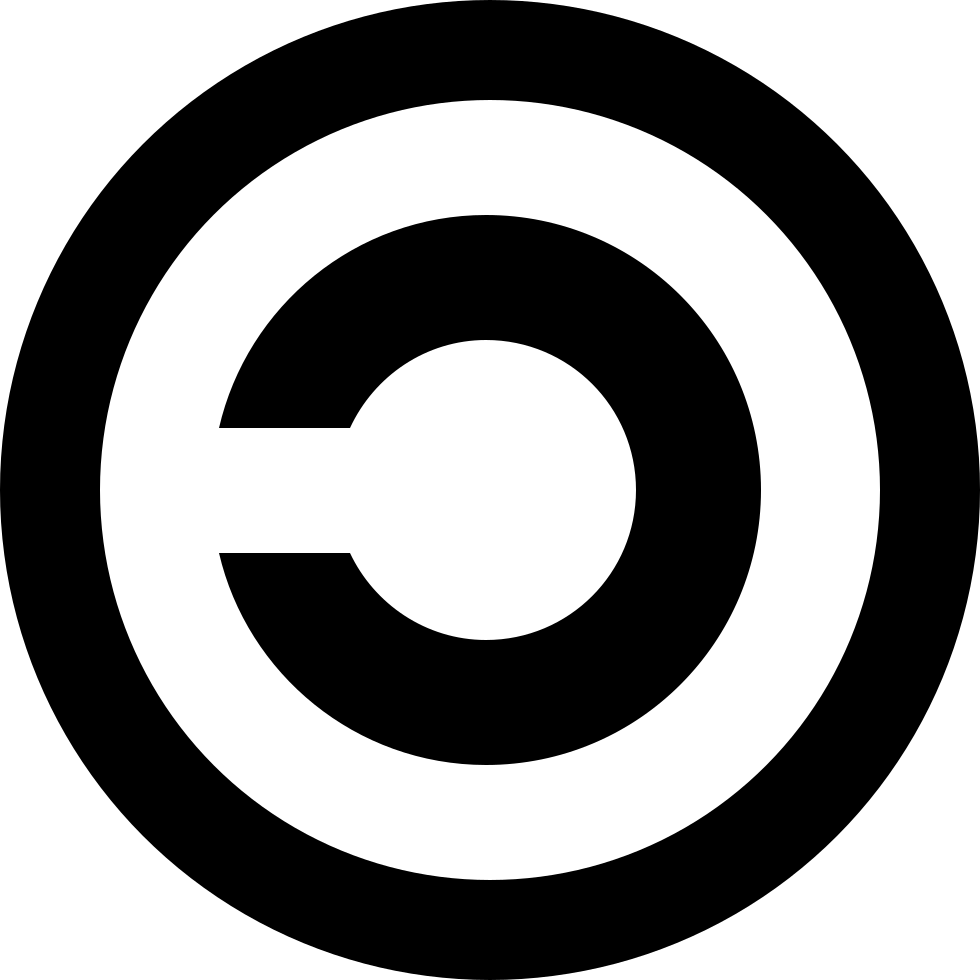
\includegraphics[width=1cm]{Copyleft.svg}
        \else
            
\includegraphics[width=1cm]{Copyleft.eps}
        \fi

Copyright (c) 2011-2012  Laurent Claessens,

Permission is granted to copy, distribute and/or modify this document under the terms of the \href{http://www.gnu.org/licenses/fdl-1.3.html}{GNU Free Documentation License}, Version 1.3 or any later version published by the Free Software Foundation; with no Invariant Sections, no Front-Cover Texts, and no Back-Cover Texts. A copy of the license is included in the section entitled ``GNU Free Documentation License''.

% Ajouter ici l'ISBN. Pour les révisions, mettre un nouvel ISBN et indiquer que c'est une révision.
% Pour l'ISBN:
% Copier tout dans un nouveau répertoire
% Créer une nouvelle branche git
% Coder en dur la date (càd enlever \today)
% Changer la licence vers non modifiable, copiable, et ajouter un lien vers la
%   version modifiable.

% http://www.bnf.fr/fr/professionnels/s_informer_obtenir_isbn/s.qu_est_ce_que_isbn.html

% TODO: écrire le README.txt

\end{center}

\clearpage


\input{laius_fdl}

\tableofcontents

% This is part of Exercices et corrigés de CdI-1
% Copyright (c) 2011
%   Laurent Claessens
% See the file fdl-1.3.txt for copying conditions.

\chapter*{Introduction}
\addcontentsline{toc}{chapter}{Introduction}

%+++++++++++++++++++++++++++++++++++++++++++++++++++++++++++++++++++++++++++++++++++++++++++++++++++++++++++++++++++++++++++
\section*{Historique}
%+++++++++++++++++++++++++++++++++++++++++++++++++++++++++++++++++++++++++++++++++++++++++++++++++++++++++++++++++++++++++++

Ces notes sont parties des exercices résolus et tapés par Yvik Swan à Bruxelles il y a bien longtemps\footnote{Une partie des sources \LaTeX\ lui sont dues.}. Avec l'aide de Nicolas Richard, toujours à Bruxelles, j'en ai fait des exercices et corrigés presque complets pour le cours de calcul différentiel et intégrale de première année en mathématique et en physique.

Vu que le cours a été remanié durant l'année 2009-2010, il n'y a plus de raisons de tenir ces notes en l'état, d'où l'idée d'en faire des notes pour le cours «outils math» de l'université de Franche-Comté. Le texte dédié à «outils math» est largement inspiré des notes manuscrites de 

% TODO: ajouter le nom.

%+++++++++++++++++++++++++++++++++++++++++++++++++++++++++++++++++++++++++++++++++++++++++++++++++++++++++++++++++++++++++++
					\section*{Ces notes sont les vôtres !}
%+++++++++++++++++++++++++++++++++++++++++++++++++++++++++++++++++++++++++++++++++++++++++++++++++++++++++++++++++++++++++


Il y a encore certainement des erreurs, des fautes de frappe et des choses pas claires. Je compte sur vous (oui : toi !) pour me signaler toute imperfection (y compris d'orthographe).

Plus vous signalez de fautes, meilleure sera la qualité du texte, et plus les étudiants de l'année prochaine vous seront reconnaissants.

%+++++++++++++++++++++++++++++++++++++++++++++++++++++++++++++++++++++++++++++++++++++++++++++++++++++++++++++++++++++++++++
					\section*{Autres notes}
%+++++++++++++++++++++++++++++++++++++++++++++++++++++++++++++++++++++++++++++++++++++++++++++++++++++++++++++++++++++++++++

Quelque sites sur lesquelles il y a des choses bonnes à lire pour tout de suite ou pour plus tard.
\begin{enumerate}
	\item
		\url{http://student.ulb.ac.be/~lclaesse/} C'est mon site. Il contient d'autres cours et exercices de math et de physique.
	\item
		\url{http://student.ulb.ac.be/~lclaesse/physique-math.pdf} Un certain nombre de pré requis qui auraient pu ou dû être vus en secondaire sont disponibles.
	\item
		\url{http://student.ulb.ac.be/~lclaesse/geog.pdf} Si vous avez besoin d'exercices de drill sur les limites, dérivées et primitives.
	\item
		\url{http://cel.archives-ouvertes.fr/} Offre de nombreux cours sur différents sujets de mathématique, physique et autres sciences. Un site à retenir; vous pourriez en avoir besoin dans les années à venir.

\end{enumerate}


\chapter{Systèmes de coordonnées}
%+++++++++++++++++++++++++++++++++++++++++++++++++++++++++++++++++++++++++++++++++++++++++++++++++++++++++++++++++++++++++++
\section{Les coordonnées cartésiennes}
%+++++++++++++++++++++++++++++++++++++++++++++++++++++++++++++++++++++++++++++++++++++++++++++++++++++++++++++++++++++++++++

Dans le plan, le choix de deux axes gradués perpendiculaires permet de repérer un point $M$ à partir de deux nombres réels $x$ et $y$, nommés \defe{abscisse}{abscisse} et \defe{ordonnées}{ordonnées} que l'on nomme les \defe{coordonnées cartésiennes}{coordonnées cartésiennes} de $M$.

Quelque exemples sur la figure \ref{LabelFigDefinitionCartesiennes}.
\newcommand{\CaptionFigDefinitionCartesiennes}{Quelque points en coordonnées cartésiennes.}
\input{Fig_DefinitionCartesiennes.pstricks}

Nous représentons alors le point par le couple $(x,y)$, et on identifie le point $M$ avec le vecteur $\overrightarrow{OM}$ qui relie l'origine $O$ des axes et le point $M$. Étant donné qu'il faut deux nombres pour repérer un point dans le plan, l'ensemble de tous les points s'identifie avec l'ensemble $\eR\times\eR=\eR^2$.

Dans l'espace, nous pouvons faire la même chose avec trois axes au lieu de deux. Les points sont alors donnés par des triples $(x,y,z)$. Étant donné qu'il faut trois nombres pour repérer un point dans l'espace, l'ensemble de tous les points de l'espace s'identifie avec l'ensemble $\eR\times\eR\times\eR=\eR^3$.

%+++++++++++++++++++++++++++++++++++++++++++++++++++++++++++++++++++++++++++++++++++++++++++++++++++++++++++++++++++++++++++
\section{Opérations sur les vecteurs}
%+++++++++++++++++++++++++++++++++++++++++++++++++++++++++++++++++++++++++++++++++++++++++++++++++++++++++++++++++++++++++++

L'\defe{addition}{addition de vecteurs} de deux vecteurs est définie par
\begin{equation}
	\begin{pmatrix}
		x	\\ 
		y	\\ 
		z	
	\end{pmatrix}+\begin{pmatrix}
		x'	\\ 
		y'	\\ 
		z'	
	\end{pmatrix}=\begin{pmatrix}
		x+x'	\\ 
		y+y'	\\ 
		z+z'	
	\end{pmatrix}.
\end{equation}
La \defe{multiplication}{multiplication de vecteurs par un scalaire} d'un vecteur $(x,y,z)$ par le scalaire $\lambda\in\eR$ est définie par
\begin{equation}
	\lambda\begin{pmatrix}
		x	\\ 
		y	\\ 
		z	
	\end{pmatrix}=\begin{pmatrix}
		\lambda x	\\ 
		\lambda y	\\ 
		\lambda z	
	\end{pmatrix}.
\end{equation}

%---------------------------------------------------------------------------------------------------------------------------
\subsection{Le produit scalaire}
%---------------------------------------------------------------------------------------------------------------------------

Le \defe{produit scalaire}{produit scalaire} entre deux vecteurs est défini par
\begin{equation}
	\begin{pmatrix}
		x	\\ 
		y	\\ 
		z	
	\end{pmatrix}\cdot\begin{pmatrix}
		x'	\\ 
		y'	\\ 
		z'	
	\end{pmatrix}=xx'+yy'+zz'.
\end{equation}
Nous utilisons souvent la notation compacte
\begin{equation}
	X=\begin{pmatrix}
		x	\\ 
		y	\\ 
		z	
	\end{pmatrix}
\end{equation}
et par conséquent nous écrivons le produit scalaire $X\cdot X'$.

\begin{proposition}[Propriétés du produit scalaire]
	Si $X$ et $Y$ sont des vecteurs de $\eR^3$, alors
	\begin{description}
		\item[Symétrie] $X\cdot Y=Y\cdot X$;
		\item[Linéarité] $(\lambda X+\mu X')\cdot Y=\lambda(X\cdot Y)+\mu(X'\cdot Y)$ pour tout $\lambda$ et $\mu$ dans $\eR$;
		\item[Défini positif] $X\cdot X\geq 0$ et $X\cdot X=0$ si et seulement si $X=0$.
	\end{description}
\end{proposition}
Note : lorsque nous écrivons $X=0$, nous voulons voulons dire $X=\begin{pmatrix}
	0	\\ 
	0	\\ 
	0	
\end{pmatrix}$.

%---------------------------------------------------------------------------------------------------------------------------
\subsection{Projection et angles}
%---------------------------------------------------------------------------------------------------------------------------

\begin{definition}
	La \defe{norme}{norme!vecteur} du vecteur $X$, notée $\| X \|$, est définie par 
	\begin{equation}
		\| X \|=\sqrt{X\cdot X}=\sqrt{x^2+y^2+z^2}
	\end{equation}
	si $X=(x,y,z)$. Cette norme sera parfois nommée «norme euclidienne».
\end{definition}
Cette définition est motivée par le théorème de Pythagore. Le nombre $X\cdot X$ est bien la longueur de la «flèche» $X$. Plus intrigante est la définition suivante :
\begin{definition}
	Deux vecteurs $X$ et $Y$ sont \defe{orthogonaux}{orthogonal!vecteur} si $X\cdot Y=0$. 
\end{definition}
Cette définition de l'orthogonalité est motivée par la proposition suivante.

\begin{proposition}		\label{PropProjScal}
	Si nous écrivons $\pr_Y$  l'opération de projection sur la droite qui sous-tend $Y$, alors nous avons
	\begin{equation}
		\| \pr_YX \|=\frac{ X\cdot Y }{ \| Y \| }.
	\end{equation}
\end{proposition}

\begin{proof}
	Les vecteurs $X$ et $Y$ sont des flèches dans l'espace. Nous pouvons choisir un système d'axe orthogonal tel que les coordonnées de $X$ et $Y$ soient
	\begin{equation}
		\begin{aligned}[]
			X&=\begin{pmatrix}
				x	\\ 
				y	\\ 
				0	
			\end{pmatrix},
			&y&=\begin{pmatrix}
				l	\\ 
				0	\\ 
				0	
			\end{pmatrix}
		\end{aligned}
	\end{equation}
	où $l$ est la longueur du vecteur $Y$. Pour ce faire, il suffit de mettre le premier axe le long de $Y$, le second dans le plan qui contient $X$ et $Y$, et enfin le troisième axe dans le plan perpendiculaire aux deux premiers.

	Un simple calcul montre que $X\cdot Y=xl+y\cdot 0+0\cdot 0=xl$. Par ailleurs, étant donné la figure \ref{LabelFigProjectionScalaire}, nous avons $\| \pr_YX \|=x$.
	\newcommand{\CaptionFigProjectionScalaire}{La longueur de la projection de $X=(x,y)$ sur $Y$ est $x$.}
	\input{Fig_ProjectionScalaire.pstricks}
	Par conséquent,
	\begin{equation}
		\| \pr_YX \|=\frac{ X\cdot Y }{ l }=\frac{ X\cdot Y }{ \| Y \| }.
	\end{equation}
\end{proof}

\begin{corollary}
	Si la norme de $Y$ est $1$, alors le nombre $X\cdot Y$ est la longueur de la projection de $X$ sur $Y$.
\end{corollary}

\begin{proof}
	Poser $\| Y \|=1$ dans la proposition \ref{PropProjScal}.
\end{proof}

Nous sommes maintenant en mesure de déterminer, pour deux vecteurs quelconques $u$ et $v$, la projection orthogonale de $u$ sur $v$. Ce sera le vecteur $\bar u$ parallèle à $v$ tel que $u-\bar u$ est orthogonal à $v$. Nous avons donc
\begin{equation}
    \bar u=\lambda v
\end{equation}
et 
\begin{equation}
    (u-\lambda v)\cdot v=0.
\end{equation}
La seconde équation donne $u\cdot v-\lambda v\cdot v=0$, ce qui fournit $\lambda$ en fonction de $u$ et $v$ :
\begin{equation}
    \lambda=\frac{ u\cdot v }{ \| v \|^2 }.
\end{equation}
Nous avons par conséquent
\begin{equation}
    \bar u=\frac{ u\cdot v }{ \| v \|^2 }v.
\end{equation}
Armés de cette interprétation graphique du produit scalaire, nous comprenons pourquoi nous disons que deux vecteurs sont orthogonaux lorsque leur produit scalaire est nul.

Nous pouvons maintenant savoir quel est le coefficient angulaire d'une droite orthogonale à une droite donnée. En effet, supposons que la première droite soit parallèle au vecteur $X$ et la seconde au vecteur $Y$. Les droites seront perpendiculaires si $X\cdot Y=0$, c'est à dire si
\begin{equation}
	\begin{pmatrix}
		x_1	\\ 
		y_1	
	\end{pmatrix}\cdot\begin{pmatrix}
		y_1	\\ 
		y_2	
	\end{pmatrix}=0.
\end{equation}
Cette équation se développe en 
\begin{equation}		\label{Eqxuyukljsca}
	x_1y_1=-x_2y_2.
\end{equation}
Le coefficient angulaire de la première droite est $\frac{ x_2 }{ x_1 }$. Isolons cette quantité dans l'équation \eqref{Eqxuyukljsca} :
\begin{equation}
	\frac{ x_2 }{ x_1 }=-\frac{ y_1 }{ y_2 }.
\end{equation}
Donc le coefficient angulaire de la première est l'inverse et l'opposé du coefficient angulaire de la seconde.

\begin{example}
	Soit la droite $d\equiv y=2x+3$. Le coefficient angulaire de cette droite est $2$. Donc le coefficient angulaire d'une droite perpendiculaires doit être $-\frac{ 1 }{ 2 }$.
\end{example}

\begin{theorem}[Inégalité de Cauchy-Schwarz]
	Si $X$ et $Y$ sont des vecteurs, alors
	\begin{equation}
		| X\cdot Y |\leq\| X \|\| Y \|.
	\end{equation}
\end{theorem}

\begin{proof}
	Étant donné que les deux membres de l'inéquation sont positifs, nous allons travailler en passant au carré afin d'éviter les racines carrés dans le second membre.
	
	Nous considérons la fonction
	\begin{equation}
		\varphi(t)=\| X+tY \|=(X+tY)\cdot(X+tY)=X\cdot X+tX\cdot Y+tY\cdot X+t^2Y\cdot Y.
	\end{equation}
	En ordonnant les termes selon les puissance de $t$,
	\begin{equation}
		\varphi(t)=\| Y \|^2t^2+2(X\cdot Y)t+\| X \|^2.
	\end{equation}
	Cela est un polynôme du second degré en $t$. Par conséquent le discriminant\footnote{Le fameux $b^2-4ac$.} doit être négatif. Nous avons donc
	\begin{equation}
		4(X\cdot Y)^2-4\| X \|^2\| Y \|^2\leq 0,
	\end{equation}
	ce qui donne immédiatement
	\begin{equation}
		(X\cdot Y)^2\leq\| X \|^2\| Y^2 \|.
	\end{equation}
	
\end{proof}

\begin{proof}[Preuve alternative]
	La preuve peut également être donnée en ne faisant pas référence au produit scalaire. Il suffit d'écrire toutes les quantités en termes des coordonnées de $X$ et $Y$. Si nous posons
	\begin{equation}
		\begin{aligned}[]
			X&=\begin{pmatrix}
				x_1	\\ 
				x_2	\\ 
				x_2	
			\end{pmatrix},
			&Y&=\begin{pmatrix}
				y_1	\\ 
				y_2	\\ 
				y_3	
			\end{pmatrix},
		\end{aligned}
	\end{equation}
	l'inégalité à prouver devient
	\begin{equation}
		(x_1y_1+x_2y_2+x_3y_3)^2\leq (x_1^2+x_2^2+x_3^2)(y_1^2+y_2^2+y_3^2).
	\end{equation}
	Nous considérons la fonction
	\begin{equation}
		\varphi(t)=(x_1+ty_1)^2+(x_2+ty_2)^2+(x_3+ty_3)^2
	\end{equation}
	En tant que norme, cette fonction est évidement positive pour tout $t$. En regroupant les termes de chaque puissance de $t$, nous avons
	\begin{equation}
		\varphi(t)=(y_1^2+y_2^2+y_3^2)t^2+2(x_1y_1+x_2y_2+x_3y_3)t+(x_1^2+x_2^2+x_3^2).
	\end{equation}
	Cela est un polynôme du second degré en $t$. Par conséquent le discriminant doit être négatif. Nous avons donc
	\begin{equation}
		4(x_1y_1+x_2y_2+x_3y_3)^2-(x_1^2+x_2^2+x_3^2)(y_1^2+y_2^2+y_3^2)\leq 0.
	\end{equation}
	La thèse en découle aussitôt.
\end{proof}

\begin{proposition}
	La norme euclidienne a les propriétés suivantes :
	\begin{enumerate}
		\item
			Pour tout vecteur $X$ et réel $\lambda$,  $\| \lambda X \|=| \lambda |\| X \|$. Attention à ne pas oublier la valeur absolue !
		\item
			Pour tout vecteurs $X$ et $Y$, $\| X+Y \|\leq \| X \|+\| Y \|$.
	\end{enumerate}
\end{proposition}

\begin{proof}
	Le premier point est l'exercice \ref{exoOutilsMath-0002}. Pour le second, nous avons les inégalités suivantes :
	\begin{subequations}
		\begin{align}
			\| X+Y \|^2&=\| X \|^2+\| Y \|^2+2X\cdot Y\\
			&\leq\| X \|^2+\| Y \|^2+2|X\cdot Y|\\
			&\leq\| X \|^2+\| Y \|^2+2\| X \|\| Y \|\\
			&=\big( \| X \|+\| Y \| \big)^2
		\end{align}
	\end{subequations}
	Nous avons utilisé d'abord la majoration $| x |\geq x$ qui est évident pour tout nombre $x$; et ensuite l'inégalité de Cauchy-Schwarz.
\end{proof}

%+++++++++++++++++++++++++++++++++++++++++++++++++++++++++++++++++++++++++++++++++++++++++++++++++++++++++++++++++++++++++++
\section{Angle entre deux vecteurs}
%+++++++++++++++++++++++++++++++++++++++++++++++++++++++++++++++++++++++++++++++++++++++++++++++++++++++++++++++++++++++++++

Si $a$ et $b$ sont des réels, l'inégalité $| a |\leq b$ peut se développer en une double inégalité
\begin{equation}
	-b\leq a\leq b.
\end{equation}
L'inégalité de Cauchy-Schwarz devient alors
\begin{equation}
	-\| X \|\| Y \|\leq X\cdot Y\leq\| X \|\| Y \|.
\end{equation}
Si $X\neq 0$ et $Y\neq 0$, nous avons alors
\begin{equation}
	-1\leq\frac{ X\cdot Y }{ \| X \|\| Y \| }\leq 1.
\end{equation}
Il existe donc un angle $\theta\in\mathopen[ 0 , \pi \mathclose]$ tel que
\begin{equation}		\label{eqDefAngleVect}
	\cos(\theta)=\frac{ X\cdot Y }{ \| X \|\| Y \| }.
\end{equation}
L'angle ainsi défini est l'\defe{angle}{angle!entre vecteurs} entre $X$ et $Y$. La définition \eqref{eqDefAngleVect} est souvent utilisée sous la forme
\begin{equation}		\label{eqPropCosThet}
	X\cdot Y=\| X \|\| Y \|\cos(\theta).
\end{equation}

Notez que les angles sont toujours des angles plus petits ou égaux à \unit{180}{\degree}.

%+++++++++++++++++++++++++++++++++++++++++++++++++++++++++++++++++++++++++++++++++++++++++++++++++++++++++++++++++++++++++++
\section{Le cercle trigonométrique}
%+++++++++++++++++++++++++++++++++++++++++++++++++++++++++++++++++++++++++++++++++++++++++++++++++++++++++++++++++++++++++++


Le \href{http://fr.wikiversity.org/wiki/Trigonométrie/Cosinus_et_sinus_dans_le_cercle_trigonométrique}{cercle trigonométrique} est le cercle de rayon $1$ représenté à la figure \ref{LabelFigCercleTrigono}. Sa longueur est $2\pi$.
\newcommand{\CaptionFigCercleTrigono}{Le cercle trigonométrique.}
\input{Fig_CercleTrigono.pstricks}

Nous verrons plus tard que la longueur de l'arc de cercle intercepté par un angle $\theta$ est égal à $\theta$. Les radians sont donc l'unité d'angle les plus adaptés au calcul de longueurs sur le cercle.

% TODO : quand le calcul de la longueur du cercle sera fait, mettre une référence ici

%---------------------------------------------------------------------------------------------------------------------------
\subsection{Les fonctions sinus et cosinus}
%---------------------------------------------------------------------------------------------------------------------------

La longueur de la projection du point $P$ sur la droite horizontale va naturellement être égale à $\cos(\theta)$. En effet, si nous notons $X$ un vecteur horizontal de norme $1$, cette projection est donné par $P\cdot X$. Mais en reprenant l'équation \eqref{eqPropCosThet}, nous voyons que
\begin{equation}
	P\cdot X=\| P \|\| X \|\cos(\theta),
\end{equation}
tandis qu'ici nous avons $\| P \|=\| X \|=1$.

Nous appelons $\sin(\theta)$ la longueur de la projection sur l'axe vertical.

Quelque dessins nous convainquent que 
\begin{equation}
	\begin{aligned}[]
		\sin(\theta+2\pi)&=\sin(\theta)&\cos(\theta+2\pi)&=\sin(\theta),\\
		\sin(\theta+\frac{ \pi }{2})&=\cos(\theta)&\cos(\theta+\frac{ \pi }{2})&=-\sin(\theta),\\
		\sin(\pi-\theta)&=\sin(\theta)&\cos(\pi-\theta)&=-\cos(\theta).
	\end{aligned}
\end{equation}
Le théorème de Pythagore nous montre aussi l'importante relation
\begin{equation}
	\sin^2(\theta)+\cos^2(\theta)=1.
\end{equation}

Quelque valeurs remarquables pour les sinus et cosinus :
\begin{equation}
	\begin{aligned}[]
		\sin 0&=0,&\sin\frac{ \pi }{ 6 }&=\frac{ 1 }{2},&\sin\frac{ \pi }{ 4 }&=\frac{ \sqrt{2} }{2},&\sin\frac{ \pi }{ 3 }&=\frac{ \sqrt{3} }{2},&\sin\frac{ \pi }{2}&=1,&\sin\pi&=0\\
		\cos 0&=1,&\cos\frac{ \pi }{ 6 }&=\frac{ \sqrt{3} }{2},&\cos\frac{ \pi }{ 4 }&=\frac{ \sqrt{2} }{2},&\cos\frac{ \pi }{ 3 }&=\frac{ 1 }{2},&\cos\frac{ \pi }{2}&=0,&\cos\pi&=-1
	\end{aligned}
\end{equation}
Voir l'exercice \ref{exoOutilsMath-0003}.

%---------------------------------------------------------------------------------------------------------------------------
\subsection{La fonction tangente}
%---------------------------------------------------------------------------------------------------------------------------

La définition de la \defe{tangente}{tangente} est :
\begin{equation}
	\tan\theta=\frac{ \sin\theta }{ \cos\theta }.
\end{equation}
Cette fonction a une interprétation géométrique donnée sur la figure \ref{LabelFigTgCercleTrigono}.
\newcommand{\CaptionFigTgCercleTrigono}{Interprétation géométrique de la fonction tangente. La tangente de l'angle $\theta$ est positive (et un peu plus grande que $1$) tandis que celle de la tangente de l'angle $\varphi$ est négative.}
\input{Fig_TgCercleTrigono.pstricks}

La restriction de la fonction tangente à l'intervalle $\mathopen] -\frac{ \pi }{2} , \frac{ \pi }{2} \mathclose[$ est une bijection vers $\eR$. Nous avons donc une fonction inverse
\begin{equation}
	\begin{aligned}
		\tan^{-1}\colon \eR&\to \mathopen] -\frac{ \pi }{2} , \frac{ \pi }{2} \mathclose[ \\
		x&\mapsto \text{$y$ tel que $\tan(y)=x$.}
	\end{aligned}
\end{equation}
Notez que cette définition, bien qu'elle ait un sens, ne dit pas comment \emph{calculer} le nombre $\tan^{-1}(x)$ pour un nombre $x$ donné\footnote{Si vous utilisez votre calculatrice, n'oubliez pas que les formules que vous connaissez ne sont valables qu'en radian.}.


%---------------------------------------------------------------------------------------------------------------------------
\subsection{Les coordonnées polaires}
%---------------------------------------------------------------------------------------------------------------------------

On a vu qu'un point $M$ dans $\eR^2$ peut être représenté par ses abscisses $x$ et ses ordonnées $y$. Nous pouvons également déterminer le même point $M$ en donnant un angle et une distance comme montré sur la figure \ref{LabelFigCoordPolaires}.
\newcommand{\CaptionFigCoordPolaires}{Un point en coordonnées polaires est donné par sa distance à l'origine et par l'angle qu'il faut avec l'horizontale.}
\input{Fig_CoordPolaires.pstricks}
Le même point $M$ peut être décrit indifféremment avec les coordonnées $(x,y)$ ou bien avec $(r,\theta)$.

\begin{remark}
	L'angle $\theta$ d'un point n'étant a priori défini qu'à un multiple de $2\pi$ près, nous convenons de toujours choisir un angle $0\leq\theta<2\pi$. Par ailleurs l'angle $\theta$ n'est pas défini si $(x,y)=(0,0)$.

	La coordonnée $r$ est toujours positive.
\end{remark}

En utilisant la trigonométrie, il est facile de trouver le changement de variable qui donne $(x,y)$ en fonction de $(r,\theta)$:
\begin{subequations}		\label{EqrthetaxyPoal}
	\begin{numcases}{}
		x=r\cos(\theta)\\
		y=r\sin(\theta).
	\end{numcases}
\end{subequations}

%///////////////////////////////////////////////////////////////////////////////////////////////////////////////////////////
\subsubsection{Transformation inverse : théorie}
%///////////////////////////////////////////////////////////////////////////////////////////////////////////////////////////

Voyons la question inverse : comment retrouver $r$ et $\theta$ si on connais $x$ et $y$ ? Tout d'abord,
\begin{equation}
	r=\sqrt{x^2+y^2}
\end{equation}
parce que la coordonnée $r$ est la distance entre l'origine et $(x,y)$. Comment trouver l'angle ? Nous supposons $(x,y)\neq (0,0)$. Si $x=0$, alors le point est sur l'axe vertical et nous avons
\begin{equation}
	\theta=\begin{cases}
		\pi/2	&	\text{si $y>0$}\\
		3\pi/2	&	 \text{si $y<0$.}
	\end{cases}
\end{equation}
Notez que si $y<0$, conformément à notre convention $\theta\geq 0$, nous avons noté $\frac{ 3\pi }{2}$ et non $-\frac{ \pi }{ 2 }$.

Supposons maintenant le cas général avec $x\neq 0$. Les équations \eqref{EqrthetaxyPoal} montrent que
\begin{equation}
	\tan(\theta)=\frac{ y }{ x }.
\end{equation}
Nous avons donc
\begin{equation}
	\theta=\tan^{-1}\left( \frac{ y }{ x } \right).
\end{equation}
La fonction inverse de la fonction tangente est celle définie plus haut.


%///////////////////////////////////////////////////////////////////////////////////////////////////////////////////////////
\subsubsection{Transformation inverse : pratique}
%///////////////////////////////////////////////////////////////////////////////////////////////////////////////////////////

Le programme suivant utilise \href{http://www.sagemath.org}{Sage}\footnote{Un module pour python} :

\VerbatimInput[tabsize=3]{calculAngle.py}

Son exécution retourne :
\begin{verbatim}
(sqrt(2), 1/4*pi)
(sqrt(5), pi - arctan(1/2))
(6, 1/6*pi)
\end{verbatim}
Notez que ce sont des valeurs \emph{exactes}. Ce ne sont pas des approximations, ce logiciel travaille de façon symbolique ! Merci donc de jeter vos vieilles calculatrices à la poubelle\footnote{Pensez au recyclage : c'est plein de métaux lourds !} : c'est de la technologie qui n'a plus cours en 2011.

%+++++++++++++++++++++++++++++++++++++++++++++++++++++++++++++++++++++++++++++++++++++++++++++++++++++++++++++++++++++++++++
\section{Coordonnées cylindriques et sphériques}
%+++++++++++++++++++++++++++++++++++++++++++++++++++++++++++++++++++++++++++++++++++++++++++++++++++++++++++++++++++++++++++

Les \defe{coordonnées cylindriques}{coordonnées!cylindrique} sont un perfectionnement des coordonnées polaires. Il s'agit simplement de donner le point $(x,y,z)$ en faisant la conversion $(x,y)\mapsto(r,\theta)$ et en gardant le $z$. Les formules de passage sont
\begin{subequations}
	\begin{numcases}{}
		x=r\cos(\theta)\\
		y=r\sin(\theta)\\
		z=z.
	\end{numcases}
\end{subequations}
Voir les exercices \ref{exoOutilsMath-0005} et \ref{exoOutilsMath-0006}.

Les \defe{coordonnées sphériques}{coordonnées!sphériques} sont ce qu'on appelle les «méridiens» et «longitudes» en géographie. Les formules de transformation sont 
\begin{subequations}		\label{SubEqsCoordSphe}
	\begin{numcases}{}
		x=\rho\sin(\theta)\cos(\varphi)\\
		y=\rho\sin(\theta)\sin(\varphi)\\
		z=\rho\cos(\theta)
	\end{numcases}
\end{subequations}
avec $0\leq\theta\leq\pi$ et $0\leq\varphi<2\pi$.

\begin{remark}
	Attention : d'un livre à l'autre les conventions sur les noms des angles changent. N'essayez donc pas d'étudier par cœur des formules concernant les coordonnées sphériques trouvées autre part. Par exemple sur le premier dessin de \href{http://fr.wikipedia.org/wiki/Coordonnées_sphériques}{wikipédia}, l'angle $\varphi$ est noté $\theta$ et l'angle $\theta$ est noté $\Phi$. Mais vous noterez que sur cette même page, les convention de noms de ces angles changent plusieurs fois.
\end{remark}

Trouvons le changement inverse, c'est à dire trouvons $\rho$, $\theta$ et $\varphi$ en termes de $x$, $y$ et $z$. D'abord nous avons
\begin{equation}
	\rho=\sqrt{x^2+y^2+z^2}.
\end{equation}
Ensuite nous savons que
\begin{equation}
	\cos(\theta)=\frac{ z }{ \rho }
\end{equation}
détermine de façon unique\footnote{Le problème $\rho=0$ ne se pose pas; pourquoi ?} un angle $\theta\in\mathopen[ 0 , \pi \mathclose]$. Dès que $\rho$ et $\theta$ sont connus, nous pouvons poser $r=\rho\sin\theta$ et alors nous nous trouvons avec les équations
\begin{subequations}
	\begin{numcases}{}
		x=r\cos(\varphi)\\
		y=r\sin(\varphi),
	\end{numcases}
\end{subequations}
qui sont similaires à celles déjà étudiées dans le cas des coordonnées polaires.

% TODO: Ajouter un texte sur les équations de plan, et pourquoi ax+by+cz+d=0 est perpendiculaire au vecteur (a,b,c).

%+++++++++++++++++++++++++++++++++++++++++++++++++++++++++++++++++++++++++++++++++++++++++++++++++++++++++++++++++++++++++++
\section{Déterminant et produit vectoriel}
%+++++++++++++++++++++++++++++++++++++++++++++++++++++++++++++++++++++++++++++++++++++++++++++++++++++++++++++++++++++++++++

%---------------------------------------------------------------------------------------------------------------------------
\subsection{Quelque propriétés du déterminant}
%---------------------------------------------------------------------------------------------------------------------------

Une \defe{matrice}{matrice} $2\times 2$ est un tableau de nombres
\begin{equation}
    \begin{pmatrix}
        a    &   b    \\ 
        c    &   d    
    \end{pmatrix}.
\end{equation}
Le \defe{déterminant}{déterminant} de cette matrice est le nombre
\begin{equation}
    \begin{vmatrix}
          a  &   b    \\ 
        c    &   d    
    \end{vmatrix}=ad-cb.
\end{equation}
Nous verrons plus tard\footnote{Et dans les années à venir.} que ce nombre contient énormément d'informations sur la matrice. Il détermine entre autres le nombre de solutions que va avoir le système d'équations linéaires associé à la matrice.

Pour une matrice $3\times 3$, nous avons le même concept, mais un peu plus compliqué. Le déterminant de la matrice
\begin{equation}
    \begin{pmatrix}
        a_{11}    &   a_{12}    &   a_{13}    \\
        a_{21}    &   a_{22}    &   a_{23}    \\
        a_{31}    &   a_{32}    &   a_{33}    
    \end{pmatrix}
\end{equation}
est le nombre
\begin{equation}
    \begin{vmatrix}
        a_{11}    &   a_{12}    &   a_{13}    \\
        a_{21}    &   a_{22}    &   a_{23}    \\
        a_{31}    &   a_{32}    &   a_{33}    
    \end{vmatrix}=
    a_{11}\begin{vmatrix}
        a_{22}  &   a_{23}    \\ 
        a_{32}    &   a_{33}    
    \end{vmatrix}+
    a_{12}\begin{vmatrix}
        a_{21}  &   a_{23}    \\ 
        a_{31}    &   a_{33}
    \end{vmatrix}+
    a_{13}\begin{vmatrix}
        a_{21}  &   a_{22}    \\ 
        a_{31}    &   a_{32}
    \end{vmatrix}.
\end{equation}


\begin{proposition}
    Si on permute deux lignes ou deux colonnes d'une matrice, alors le déterminant change de signe.
\end{proposition}

\begin{proposition}
    Si on multiplie une ligne ou une colonne d'une matrice par un nombre $\lambda$, alors le déterminant est multiplié par $\lambda$.
\end{proposition}

\begin{proposition}
    Si deux lignes ou deux colonnes sont proportionnelles, alors le déterminant est nul.
\end{proposition}

\begin{proposition}
    Si on ajoute à une ligne une combinaison linéaire des autres lignes, alors le déterminant ne change pas (idem pour les colonnes).
\end{proposition}

%---------------------------------------------------------------------------------------------------------------------------
\subsection{Produit vectoriel}
%---------------------------------------------------------------------------------------------------------------------------

Une application importante du déterminant $3\times 3$ est qu'il détermine le \defe{produit vectoriel}{produit!vectoriel} entre deux vecteurs. Pour cela nous introduisons les vecteurs de base
\begin{equation}
    \begin{aligned}[]
        1_x&=\begin{pmatrix}
            1    \\ 
            0    \\ 
            0    
        \end{pmatrix}
        ,&1_y=\begin{pmatrix}
            0    \\ 
            1    \\ 
            0    
        \end{pmatrix},&1_z&=\begin{pmatrix}
            0    \\ 
            0    \\ 
            1    
        \end{pmatrix}.
    \end{aligned}
\end{equation}
Ensuite, si $v$ et $w$ sont des vecteurs dans $\eR^3$, nous définissons
\begin{equation}
    \begin{aligned}[]
        \begin{pmatrix}
            v_x    \\ 
            v_y    \\ 
            v_z    
        \end{pmatrix}\times\begin{pmatrix}
            w_x    \\ 
            w_y    \\ 
            w_z    
        \end{pmatrix}=
        \begin{vmatrix}
              1_x  &   1_y    &   1_z    \\
              v_x  &   v_y    &   v_z    \\
              w_x  &   w_y    &   w_z    \\
        \end{vmatrix}&=
        (v_yw_z-w_yvz)1_x\\
        &-(v_xw_z-w_xvz)1_y\\
        &+(v_xw_y-w_xvy)1_z\in\eR^3
    \end{aligned}
\end{equation}

Ce produit vectoriel peut aussi être écrit sous la forme
\begin{equation}        \label{EqProdVectEspilonijk}
    v\times w=\sum_{i,j,k}\epsilon_{ijk}v_iw_j1_k
\end{equation}
où $\epsilon_{ijk}$ est défini par $\epsilon_{xyz}=1$ et ensuite $\epsilon_{ijk}$ est $1$ ou $-1$ suivant que la permutation des $x$, $y$ et $z$ est paire ou impaire.

Un grand intérêt du produit vectoriel est qu'il fournit un vecteur qui est simultanément perpendiculaire aux deux vecteurs donnés.
\begin{proposition}
    Le vecteur $v\times w$ est perpendiculaire à $v$ et à $w$.
\end{proposition}

\begin{proposition}
    Le produit vectoriel est une opération antisymétrique, c'est à dire
    \begin{equation}
        v\times w=-w\times v.
    \end{equation}
    En particulier $v\times v=0$ pour tout vecteur $v\in\eR^3$.
\end{proposition}

\begin{proposition}
    Le produit vectoriel est linéaire. Pour tout vecteurs $a$, $b$, $c$ et pour tout nombre $\alpha$ et $\beta$ nous avons
    \begin{equation}
        \begin{aligned}[]
            a\times (\alpha b +\beta c)&=\alpha(a\times b)+\beta(a\times c)\\
            (\alpha a+\beta b)\times c&=\alpha(a\times c)+\beta(b\times c).
        \end{aligned}
    \end{equation}
\end{proposition}

Les trois vecteurs de base $1_x$, $1_y$ et $1_y$ ont des produits vectoriels faciles à retenir :
\begin{equation}
    \begin{aligned}[]
        1_x\times 1_y&=1_z\\
        1_y\times 1_z&=1_x\\
        1_z\times 1_x&=1_y
    \end{aligned}
\end{equation}

\begin{example}
    Calculons le produit vectoriel $v\times w$ avec
    \begin{equation}
        \begin{aligned}[]
            v&=\begin{pmatrix}
                3    \\ 
                -1    \\ 
                1    
            \end{pmatrix}&w=\begin{pmatrix}
                1    \\ 
                2    \\ 
                -1    
            \end{pmatrix}.
        \end{aligned}
    \end{equation}
    Les vecteurs s'écrivent sous la forme $v=31_x-1_y+1_z$ et $w=1_x+21_y-1_z$. Le produit vectoriel s'écrit
    \begin{equation}
        \begin{aligned}[]
            (31_x-1_y+1_z)\times (1_x+21_y-1_z)&=61_x\times 1_y-31_x\times 1_z\\
                                &\quad -1_y\times 1_x + 1_y\times 1_z\\
                                &\quad + 1_z\times 1_x + 21_z\times 1_y\\
                                &=61_z+31_y+1_z+1_x+1_y-21_x\\
                                &=-1_x+41_y+71_z.
        \end{aligned}
    \end{equation}
\end{example}

%---------------------------------------------------------------------------------------------------------------------------
\subsection{Produit mixte}
%---------------------------------------------------------------------------------------------------------------------------

Si $a$, $b$ et $c$ sont trois vecteurs, leur \defe{produit mixte}{produit!mixte} est le nombre $a\cdot(b\times c)$. En écrivant le produit vectoriel sous forme de somme de trois déterminants $2\times 2$, nous avons
\begin{equation}
    \begin{aligned}[]
        a\cdot& (b\times c)\\&=(a_11_x+a_21_y+a_31_z)\cdot\left(
        \begin{vmatrix}
            b_2    &   b_3    \\ 
            c_2    &   c_3    
        \end{vmatrix}1_x-\begin{vmatrix}
            b_1    &   b_3    \\ 
            c_1    &   c_3    
        \end{vmatrix}1_y+\begin{vmatrix}
            b_1    &   b_2    \\ 
            c_1    &   c_2    
        \end{vmatrix}\right)\\
        &=a_1\begin{vmatrix}
            b_2    &   b_3    \\ 
            c_2    &   c_3    
        \end{vmatrix}-a_2\begin{vmatrix}
            b_1    &   b_3    \\ 
            c_1    &   c_3    
        \end{vmatrix}+a_3\begin{vmatrix}
            b_1    &   b_2    \\ 
            c_1    &   c_2    
        \end{vmatrix}\\
        &=\begin{vmatrix}
            a_1    &   a_2    &   a_3    \\
            b_1    &   b_2    &   b_3    \\
            c_1    &   c_2    &   c_3
        \end{vmatrix}.
    \end{aligned}
\end{equation}
Le produit mixte s'écrit donc sous forme d'un déterminant. Nous retenons cette formule:
\begin{equation}        \label{EqProduitMixteDet}
    a\cdot (b\times c)=\begin{vmatrix}
        a_1    &   a_2    &   a_3    \\
        b_1    &   b_2    &   b_3    \\
        c_1    &   c_2    &   c_3
    \end{vmatrix}.
\end{equation}


\begin{proposition}
    Le produit vectoriel $a\times b$ est un vecteur orthogonal à $a$ et $b$.
\end{proposition}

\begin{proof}
    Vérifions que $a\perp (a\times b)$. Pour cela, nous calculons $a\cdot (a\times b)$, c'est à dire le produit mixte
    \begin{equation}
        a\cdot(a\times b)=\begin{vmatrix}
            a_1    &   a_2    &   a_3    \\
            a_1    &   a_2    &   a_3    \\
            b_1    &   b_2    &   b_3
        \end{vmatrix}=0.
    \end{equation}
    L'annulation de ce déterminant est due au fait que deux de ses lignes sont égales.
\end{proof}

\begin{proposition}     \label{PropNormeProdVectoabsint}
    Nous avons
    \begin{equation}
        \| a\times b \|=\| a \|\| b \|\sin(\theta)
    \end{equation}
    où $\theta\in\mathopen[ 0.\pi \mathclose]$ est l'angle formé par $a$ et $b$.
\end{proposition}

\begin{proof}
    En utilisant la décomposition du produit vectoriel, nous avons
    \begin{equation}
        \begin{aligned}[]
            \| a\times b \|^2&=\begin{vmatrix}
                a_2    &   a_3    \\ 
                b_2    &   b_3    
            \end{vmatrix}^2+\begin{vmatrix}
                a_1    &   a_3    \\ 
                c_1    &   b_3    
            \end{vmatrix}^2+\begin{vmatrix}
                a_1    &   a_2    \\ 
                b_1    &   b_2    
            \end{vmatrix}^2\\
            &=(a_2b_2-b_2a_3)^2+(a_1b_3-a_3b_1)^2+(a_1b_2-a_2b_1)^2\\
            &=(a_1^2+a_2^2+a_3^2)(b_1^2+b_2^2+b_3^2)-(a_1b_1+a_2b_2+a_3b_3)^2\\
            &=\| a \|^2\| b \|^2-(a\times b)^2\\
            &=\| a \|^2\| b \|^2-\| a \|^2\| b \|^2\cos^2(\theta)\\
            &=\| a \|^2\| b \|^2\big( 1-\cos^2(\theta) \big)\\
            &=\| a \|^2\| b \|^2\sin(\theta).
        \end{aligned}
    \end{equation}
    D'où le résultat.
\end{proof}

\begin{remark}      \label{RemaAireParalProdVect}
    Le nombre $\| a \|\| b \|\sin(\theta)$ est l'aire du parallélogramme formé par les vecteurs $a$ et $b$, comme cela se voit sur la figure \ref{LabelFigParallelogramme}.
    \newcommand{\CaptionFigParallelogramme}{Calculer l'aire d'un parallélogramme.}
    \input{Fig_Parallelogramme.pstricks}
\end{remark}

%---------------------------------------------------------------------------------------------------------------------------
\subsection{Interprétation géométrique du déterminant}
%---------------------------------------------------------------------------------------------------------------------------

%///////////////////////////////////////////////////////////////////////////////////////////////////////////////////////////
\subsubsection{Déterminant de dimension deux}
%///////////////////////////////////////////////////////////////////////////////////////////////////////////////////////////

La valeur absolue du déterminant 
\begin{equation}        \label{EqDeratb}
    \begin{vmatrix}
        a_1    &   a_2    \\ 
        b_1    &   b_2    
    \end{vmatrix}
\end{equation}
est l'aire du parallélogramme déterminé par les vecteurs $\begin{pmatrix}
    a_1    \\ 
    a_2    
\end{pmatrix}$ et $\begin{pmatrix}
    b_1    \\ 
    b_2    
\end{pmatrix}$. En effet, d'après la remarque \ref{RemaAireParalProdVect}, l'aire de ce parallélogramme est donnée par la norme du produit vectoriel
\begin{equation}
    \begin{pmatrix}
        a_1    \\ 
        a_2    \\ 
        0    
    \end{pmatrix}\times
    \begin{pmatrix}
          b_1  \\ 
        b_2    \\ 
        0    
    \end{pmatrix}=\begin{vmatrix}
        1_x    &   1_y    &   1_z    \\
        a_1    &   a_2    &   0    \\
        b_1    &   b_2    &   0
    \end{vmatrix}=
    \begin{vmatrix}
        a_1    &   a_2    \\ 
        b_1    &   b_2    
    \end{vmatrix}1_z,
\end{equation}
donc la norme $\| a\times b \|$ est bien donnée par la valeur absolue du déterminant \eqref{EqDeratb}.

%///////////////////////////////////////////////////////////////////////////////////////////////////////////////////////////
\subsubsection{Déterminant de dimension trois}
%///////////////////////////////////////////////////////////////////////////////////////////////////////////////////////////

Si les vecteurs $a$, $b$ et $c$ sont sont pas coplanaires, alors la valeur absolue du produit mixte (voir équation \eqref{EqProduitMixteDet}) $a\cdot(b\times c)$ donne le volume du parallélépipède construit sur les vecteurs $a$, $b$ et $c$.

En effet si $\varphi$ est l'angle entre $b\times c$ et $a$, alors la hauteur du parallélépipède vaut $\| a \|\cos(\varphi)$. En effet la direction verticale est donnée par $b\times c$, et la hauteur est alors la «composante verticale» de $a$. Par conséquent, étant donné que $\| b\times c \|$ est la surface de la base, le volume du parallélépipède vaut
\begin{equation}
    V=\| b\times c\|  \| a \|\cos(\varphi).
\end{equation}
Or cette formule est le produit scalaire de $a$ par $b \times c$; ce dernier étant donné par le déterminant de la matrice formée des composantes de $a$, $b$ et $c$ grâce à la formule \eqref{EqProduitMixteDet}.



\chapter{Exercices outils math}
% This is part of Mes notes de mathématique
% Copyright (c) 2011-2012
%   Laurent Claessens
% See the file fdl-1.3.txt for copying conditions.

%---------------------------------------------------------------------------------------------------------------------------
\subsection{Trigonométrie}
%---------------------------------------------------------------------------------------------------------------------------

\Exo{OutilsMath-0003}
\Exo{OutilsMath-0004}

%---------------------------------------------------------------------------------------------------------------------------
\subsection{Dérivées de fonctions de une variable}
%---------------------------------------------------------------------------------------------------------------------------

\Exo{Derive-0001}  
\Exo{Derive-0002}  
\Exo{Derive-0004}  
\Exo{Derive-0005}  
\Exo{Derive-0006}  
\Exo{Derive-0007}  
\Exo{OutilsMath-0027}
\Exo{OutilsMath-0028}
\Exo{OutilsMath-0029}
\Exo{OutilsMath-0048}
\Exo{OutilsMath-0056}
\Exo{OutilsMath-0039}
\Exo{OutilsMath-0088}

% Maximisation
\Exo{OutilsMath-0040}
\Exo{OutilsMath-0050}

%---------------------------------------------------------------------------------------------------------------------------
\subsection{Vecteurs}
%---------------------------------------------------------------------------------------------------------------------------

\Exo{Derive-0003}  
\Exo{OutilsMath-0047}
\Exo{OutilsMath-0001}
\Exo{OutilsMath-0002} 
\Exo{OutilsMath-0016}
\Exo{OutilsMath-0017}
\Exo{OutilsMath-0069}
\Exo{OutilsMath-0071}
\Exo{OutilsMath-0072}
\Exo{OutilsMath-0074}

%---------------------------------------------------------------------------------------------------------------------------
\subsection{Conversions entre les systèmes de coordonnées}
%---------------------------------------------------------------------------------------------------------------------------

\Exo{OutilsMath-0018}
\Exo{OutilsMath-0019}
\Exo{OutilsMath-0014}
\Exo{OutilsMath-0023}
\Exo{OutilsMath-0005}
\Exo{OutilsMath-0008}
\Exo{OutilsMath-0007}
\Exo{OutilsMath-0006}
\Exo{OutilsMath-0009}
\Exo{OutilsMath-0010}
\Exo{OutilsMath-0011}

\Exo{OutilsMath-0049}
\Exo{OutilsMath-0038}
\Exo{OutilsMath-0020}
\Exo{OutilsMath-0021}


\Exo{OutilsMath-0012}
\Exo{OutilsMath-0013}
\Exo{OutilsMath-0015}

\Exo{OutilsMath-0024}
\Exo{OutilsMath-0025}
\Exo{OutilsMath-0026}

%---------------------------------------------------------------------------------------------------------------------------
\subsection{Gradients, dérivées et différentielles}
%---------------------------------------------------------------------------------------------------------------------------

\Exo{OutilsMath-0030}
\Exo{OutilsMath-0031}
\Exo{OutilsMath-0032}
\Exo{OutilsMath-0033}
\Exo{OutilsMath-0054}

\Exo{OutilsMath-0037}
\Exo{OutilsMath-0130}
\Exo{OutilsMath-0059}
\Exo{OutilsMath-0022}

\Exo{OutilsMath-0041}
\Exo{OutilsMath-0042}
\Exo{OutilsMath-0043}
\Exo{OutilsMath-0055}
\Exo{OutilsMath-0044}
\Exo{OutilsMath-0045}
\Exo{OutilsMath-0089}


\Exo{Derive-0008}  

%---------------------------------------------------------------------------------------------------------------------------
\subsection{Plans tangents}
%---------------------------------------------------------------------------------------------------------------------------

\Exo{OutilsMath-0046}
\Exo{OutilsMath-0057}

%---------------------------------------------------------------------------------------------------------------------------
\subsection{Travail, circulation, intégration sur un chemin}
%---------------------------------------------------------------------------------------------------------------------------

\Exo{OutilsMath-0051}
\Exo{OutilsMath-0052}
\Exo{OutilsMath-0061}
\Exo{OutilsMath-0063}
\Exo{OutilsMath-0098}
\Exo{OutilsMath-0064}
\Exo{OutilsMath-0062}
\Exo{OutilsMath-0060}
\Exo{OutilsMath-0090}
\Exo{OutilsMath-0095}
\Exo{OutilsMath-0096}

\Exo{OutilsMath-0143}

%---------------------------------------------------------------------------------------------------------------------------
\subsection{Rotationnel}
%---------------------------------------------------------------------------------------------------------------------------

\Exo{OutilsMath-0034}
\Exo{OutilsMath-0035}
\Exo{OutilsMath-0036}
\Exo{OutilsMath-0053}
\Exo{OutilsMath-0058}
\Exo{OutilsMath-0065}
\Exo{OutilsMath-0066}
\Exo{OutilsMath-0067}
\Exo{OutilsMath-0068}
\Exo{OutilsMath-0091}
\Exo{OutilsMath-0097}

%---------------------------------------------------------------------------------------------------------------------------
\subsection{Produit vectoriel, déterminants, surfaces et volumes}
%---------------------------------------------------------------------------------------------------------------------------

\Exo{OutilsMath-0070}
\Exo{OutilsMath-0099}
\Exo{OutilsMath-0075}
\Exo{OutilsMath-0076}
\Exo{OutilsMath-0073}

%---------------------------------------------------------------------------------------------------------------------------
\subsection{Coordonnées curvilignes}
%---------------------------------------------------------------------------------------------------------------------------

\Exo{OutilsMath-0077}
\Exo{OutilsMath-0078}
\Exo{OutilsMath-0079}
\Exo{OutilsMath-0080}
\Exo{OutilsMath-0081}
\Exo{OutilsMath-0082}
\Exo{OutilsMath-0083}
\Exo{OutilsMath-0084}

%---------------------------------------------------------------------------------------------------------------------------
\subsection{Intégrales de fonctions}
%---------------------------------------------------------------------------------------------------------------------------

\Exo{OutilsMath-0115}
\Exo{OutilsMath-0092}
\Exo{OutilsMath-0093}
\Exo{OutilsMath-0094}
\Exo{OutilsMath-0101}

\Exo{OutilsMath-0102}
\Exo{OutilsMath-0103}
\Exo{OutilsMath-0104}
\Exo{OutilsMath-0105}
\Exo{OutilsMath-0106}
\Exo{OutilsMath-0107}
\Exo{OutilsMath-0108}
\Exo{OutilsMath-0116}
\Exo{OutilsMath-0117}
\Exo{OutilsMath-0118}

\Exo{OutilsMath-0144}
\Exo{OutilsMath-0145}

%---------------------------------------------------------------------------------------------------------------------------
\subsection{Intégration de champs de vecteurs}
%---------------------------------------------------------------------------------------------------------------------------

\Exo{OutilsMath-0113}
\Exo{OutilsMath-0114}
\Exo{OutilsMath-0109}
\Exo{OutilsMath-0110}
\Exo{OutilsMath-0111}
\Exo{OutilsMath-0112}


%---------------------------------------------------------------------------------------------------------------------------
\subsection{Interrogations, DS, examens 2010-2011}
%---------------------------------------------------------------------------------------------------------------------------

Les questions suivantes ont été posées durant l'année 2010-2011.

\Exo{OutilsMath-0119}
\Exo{OutilsMath-0120}
\Exo{OutilsMath-0121}
\Exo{OutilsMath-0122}
\Exo{OutilsMath-0123}
\Exo{OutilsMath-0124}
\Exo{OutilsMath-0125}
\Exo{OutilsMath-0126}
\Exo{OutilsMath-0127}
\Exo{OutilsMath-0128}
\Exo{OutilsMath-0129}
\Exo{OutilsMath-0085}
\Exo{OutilsMath-0100}
\Exo{OutilsMath-0086}
\Exo{OutilsMath-0087}
\Exo{OutilsMath-0137}
\Exo{OutilsMath-0138}


%---------------------------------------------------------------------------------------------------------------------------
\subsection{DM 2011-2012}
%---------------------------------------------------------------------------------------------------------------------------

\Exo{OutilsMath-0131}
\Exo{OutilsMath-0132}
\Exo{OutilsMath-0133}
\Exo{OutilsMath-0134}
\Exo{OutilsMath-0135}
\Exo{OutilsMath-0136}

%---------------------------------------------------------------------------------------------------------------------------
\subsection{Interrogation mars 2012}
%---------------------------------------------------------------------------------------------------------------------------

\Exo{reserve0007}
\Exo{reserve0008}
\Exo{reserve0009}
\Exo{reserve0010}

%---------------------------------------------------------------------------------------------------------------------------
\subsection{DS avril 2012}
%---------------------------------------------------------------------------------------------------------------------------

\Exo{examens-0002}
\Exo{examens-0003}
\Exo{examens-0004}
\Exo{examens-0005}

%---------------------------------------------------------------------------------------------------------------------------
\subsection{Interrogation mai 2012}
%---------------------------------------------------------------------------------------------------------------------------

\Exo{OutilsMath-0139}
\Exo{OutilsMath-0140}
\Exo{OutilsMath-0141}
\Exo{OutilsMath-0142}


\chapter{Rappels de CdI}
% This is part of Exercices et corrigés de CdI-1
% Copyright (c) 2011
%   Laurent Claessens
% See the file fdl-1.3.txt for copying conditions.

%+++++++++++++++++++++++++++++++++++++++++++++++++++++++++++++++++++++++++++++++++++++++++++++++++++++++++++++++++++++++++++
					\section{Binôme de Newton}
%+++++++++++++++++++++++++++++++++++++++++++++++++++++++++++++++++++++++++++++++++++++++++++++++++++++++++++++++++++++++++++

\begin{proposition}
Pour tout $x$, $y\in\eR$ et $n\in\eN$, nous avons
\begin{equation}		\label{EqNewtonB}
	(x+y)^n=\sum_{k=0}^n{n\choose k}x^{n-k}y^k
\end{equation}
où
\begin{equation}
	{n\choose k}=\frac{ n! }{ k!(n-k)! }
\end{equation}
sont les \defe{coefficients binomiaux}{Coefficients binomiaux}.
\end{proposition}

La preuve qui suit provient de \href{http://fr.wikipedia.org/wiki/Formule_du_binôme_de_Newton}{wikipédia}.
\begin{proof}
La preuve se fait par récurrence. La vérification pour $n=0$ et $n=1$ sont faciles. Supposons que la formule \eqref{EqNewtonB} soit vraie pour $n$, et prouvons la pour $n+1$. Nous avons
\begin{equation}		\label{EqBinTrav}
	\begin{aligned}[]
		(x+y)^{n+1}	&=(x+y)\cdot  \sum_{k=0}^n{n\choose k}x^{n-k}y^k\\
				&= \sum_{k=0}^n{n\choose k}x^{n-k+1}y^k+\sum_{k=0}^n{n\choose k}x^{n-k}y^{k+1}\\
				&=x^{n+1}+ \sum_{k=1}^n{n\choose k}x^{n-k+1}y^k+\sum_{k=0}^{n-1}{n\choose k}x^{n-k}y^{k+1}+y^{n+1}.
	\end{aligned}
\end{equation}
La seconde grande somme peut être transformée en posant $i=k+1$ :
\begin{equation}
	\sum_{k=0}^{n-1}{n\choose k}x^{n-k}y^{k+1}	=\sum_{i=1}^n{n\choose i-1}x^{n-(i-1)}y^{i-1+1},
\end{equation}
dans lequel nous pouvons immédiatement renommer $i$ par $k$. En remplaçant dans la dernière expression de \eqref{EqBinTrav}, nous trouvons
\begin{equation}
	(x+y)^{n+1}=x^{n+1}+y^{n+1}+\sum_{k=1}^n\left[ {n\choose k}+{n\choose k-1} \right]x^{n-k+1}y^k.
\end{equation}
La thèse découle maintenant de la formule
\begin{equation}
	{n\choose k}+{n\choose k-1}={n+1\choose k}
\end{equation}
qui est vraie parce que
\begin{equation}
	\frac{ n! }{ k!(n-k)! }+\frac{ n! }{ (k-1)(n-k+1)! }=\frac{ n!(n-k+1)+n!k }{ k!(n-k+1)! }=\frac{ n!(n+1) }{  k!(n-k+1)!  },
\end{equation}
par simple mise au même dénominateur.
\end{proof}


 \section{Les nombres complexes}
 \subsection{Définitions de base}
 Un nombre complexe s'écrit sous la forme $z = a + b i$, où $a$ et $b$
 sont des nombres réels appelés (et notés) respectivement partie réelle
 ($a = \Re(z)$) et partie imaginaire ($b = \Im(z)$) de $z$. L'ensemble
 des nombres de cette forme s'appelle l'ensemble des nombres complexes
 ; cet ensemble porte une structure de corps et est noté $\CC$. Le
 nombre complexe $i = 0 + 1 i$ est un nombre imaginaire qui a la
 particularité que $i^2 = -1$.

 Deux nombres complexes $a + bi$ et $c + di$ sont égaux si et seulement
 si $a = c$ et $b = d$, c'est-à-dire leurs parties réelles sont égales,
 et leurs parties imaginaires sont égales.

 Un nombre complexe étant représenté par deux nombres, on peut le
 représenter dans un plan appelé « plan de Gauss ». La plupart des
 opérations sur les nombres complexes ont leur interprétation
 géométrique dans ce plan.

 Pour $z = a + bi$ un nombre complexe, on note $\bar z = a - bi$ le
 \Defn{complexe conjugué} de $z$. Dans le plan de Gauss, il s'agit du
 symétrique de $z$ par rapport à la droite réelle (généralement
 dessinée horizontalement).

 On définit le module du complexe $z$ par $\module z = \sqrt{z\bar z} =
 \sqrt{a^2 + b^2}$. Dans le plan de Gauss, il s'agit de la distance
 entre $0$ et $z$.

 \begin{proposition}
Pour tout $z = a+bi$ et $z^\prime$ nombres complexes, on a
   \begin{enumerate}
   \item $z \bar z = a^2 + b^2$;
   \item $\bar{\bar{z}} = z$;
   \item $\module z = \module {\bar z}$;
   \item $\module{zz^\prime} = \module z \module{z^\prime}$;
   \item $\module{z+z^\prime} \leq \module z + \module{z^\prime}$.
   \end{enumerate}
 \end{proposition}

 \subsection{Forme polaire ou trigonométrique}
 Dans le plan de Gauss, le module d'un complexe $z$ représente la
 distance entre $0$ et $z$. On appelle \Defn{argument} de $z$ (noté
 $\arg z$) l'angle (déterminé à $2\pi$ près) entre le demi-axe des
 réels positifs et la demi-droite qui part de $0$ et passe par $z$. Le
 module et l'argument d'un complexe permettent de déterminer
 univoquement ce complexe puisqu'on a la formule
 \[z = a + bi = \module z \left( \cos(\arg(z)) + i \sin(\arg(z))
 \right)\]

 L'argument de $z$ se détermine via les formules
 \[\frac a {\module z} = \cos(\arg(z)) \quad \frac b {\module z} =
 \sin(\arg(z))\] ou encore par la formule
 \[\frac b a = \tan(\arg(z)) \quad \text{en vérifiant le
   quadrant.}\]%
 La vérification du quadrant vient de ce que la tangente ne détermine
 l'angle qu'à $\pi$ près.



% This is part of Mes notes de mathématique
% Copyright (c) 2011-2012
%   Laurent Claessens
% See the file fdl-1.3.txt for copying conditions.



%+++++++++++++++++++++++++++++++++++++++++++++++++++++++++++++++++++++++++++++++++++++++++++++++++++++++++++++++++++++++++++
					\section{Maximisation sans contraintes}
%+++++++++++++++++++++++++++++++++++++++++++++++++++++++++++++++++++++++++++++++++++++++++++++++++++++++++++++++++++++++++++

%---------------------------------------------------------------------------------------------------------------------------
					\subsection{Fonctions à une seule variable}
%---------------------------------------------------------------------------------------------------------------------------

\begin{definition}
Soit $f\colon A\subset \eR\to \eR$ et $a\in A$. Le point $a$ est un \defe{maximum local}{Maximum!local} de $f$ si il existe un voisinage $\mU$ de $a$ tel que $f(a)\geq f(x)$ pour tout $x\in\mU\cap A$. Le point $a$ est un \defe{maximum global}{Maximum!global} si $f(a)\geq g(x)$ pour tout $x\in A$.
\end{definition}

La proposition basique à utiliser lors de la recherche d'extrema est la suivante :
\begin{proposition}
Soit $f\colon A\subset\eR\to \eR$ et $a\in\Int(A)$. Supposons que $f$ est dérivable en $a$. Si $a$ est un \href{http://fr.wikipedia.org/wiki/Extremum}{extremum} local, alors $f'(a)=0$.
\end{proposition}

La réciproque n'est pas vraie, comme le montre l'exemple de la fonction $x\mapsto x^3$ en $x=0$ : sa dérivée est nulle et pourtant $x=0$ n'est ni un maximum ni un minimum local. 

Cette proposition ne sert donc qu'à sélectionner des \emph{candidats} extremum. Afin de savoir si ces candidats sont des extrema, il y a la proposition suivante (proposition 1, page 227).

\begin{proposition}
Soit $f\colon I\subset \eR\to \eR$, une fonction de classe $C^k$ au voisinage d'un point $a\in\Int I$. Supposons que
\begin{equation}
	f'(a)=f''(a)=\ldots=f^{(k-1)}(a)=0,
\end{equation}
et que
\begin{equation}
	f^{(k)}(a)\neq 0.
\end{equation}
Dans ce cas,
\begin{enumerate}

\item
Si $k$ est pair, alors $a$ est un point d'extremum local de $f$, c'est un minimum si $f^{(k)}(a)>0$, et un maximum si $f^{(k)}(a)<0$,
\item
Si $k$ est impair, alors $a$ n'est pas un extremum local de $f$.

\end{enumerate}
\end{proposition}

Note : jusqu'à présent nous n'avons rien dit des extrema \emph{globaux} de $f$. Il n'y a pas grand chose à en dire. Si un point d'extremum global est situé dans l'intérieur du domaine de $f$, alors il sera extremum local (a fortiori). Ou alors, le maximum global peut être sur le bord du domaine. C'est ce qui arrive à des fonctions strictement croissantes sur un domaine compact.

Une seule certitude : si une fonction est continue sur un compact, elle possède une minimum et un maximum global.

%---------------------------------------------------------------------------------------------------------------------------
					\subsection{Fonctions à plusieurs variables}
%---------------------------------------------------------------------------------------------------------------------------


%---------------------------------------------------------------------------------------------------------------------------
					\subsection{Quelque mots à propos de matrices}
%---------------------------------------------------------------------------------------------------------------------------

Les notions qui suivent seront vues au cours de géométrie lorsqu'il sera temps. 

Si $g$ est une application bilinéaire sur $\eR^2$, nous disons qu'elle est
\begin{enumerate}

\item
\defe{Définie positive}{Application!définie positive} si $g(u,u)\geq 0$ pour tout $u\in\eR^2$ et $g(u,u)=0$ si et seulement si $u=0$.

\item
\defe{semi-définie positive}{Application!semi-définie positive} si $g(u,u)\geq 0$ pour tout $u\in\eR^2$. 

\end{enumerate}

Une matrice $M$ est définie positive si $v^tMv>0$ pour tout $v\neq 0$, en particulier si $v$ est un vecteur propre de valeur propre $\lambda$ (c'est à dire si $Mv=\lambda v$), alors $\lambda v^tv>0$, et donc $\lambda>0$. Donc $M$ sera définie positive si toutes ses valeurs propres sont positives.

\begin{proposition}
	Soit $M$, une matrice $2\times 2$ symétrique\footnote{la matrice $d^2f(a)$ est toujours symétrique quand $f$ est de classe $C^2$.}. Nous avons
	\begin{enumerate}
		\item
		$\det M>0$ et $\tr(M)>0$ implique $M$ définie positive,
		\item
		$\det M>0$ et $\tr(M)<0$ implique $M$ définie négative,
		\item
		$\det M<0$ implique ni semi définie positive, ni définie négative (et donc pas un extrema dans le cas où $M=d^2f(a)$ par le point \ref{ItemPropoExtreRn} de la proposition \ref{PropoExtreRn}),
		\item
		$\det M=0$ implique $M$ semi-définie positive ou semi-définie négative.
	\end{enumerate}
\end{proposition}
 

%---------------------------------------------------------------------------------------------------------------------------
					\subsection{Les théorèmes}
%---------------------------------------------------------------------------------------------------------------------------



Un point $a$ à l'intérieur du domaine d'une fonction $f\colon A\subset\eR^n\to \eR$ est une \defe{point critique}{Critique!point} de $f$ lorsque $df(a)=0$. Ces points sont analogues aux points où la dérivée d'une fonction sur $\eR$ s'annule. Les points critiques de $f$ sont dons les candidats à être des points d'extremum.

\begin{proposition}		\label{PropoExtreRn}
Soit $f\colon A\subset\eR^n\to \eR$ une fonction de classe $C^2$ au voisinage de $a\in\Int(A)$.
\begin{enumerate}

\item
Si $a$ est un point critique de $f$, et si $d^2f(a)$ est \href{http://fr.wikipedia.org/wiki/Matrice_définie_positive}{définie positive}, alors $a$ est un minimum local strict de $f$,
\item		\label{ItemPropoExtreRn}
Si $a$ est un minimum local, alors $a$ est un point critique et $d^2f(a)$ est semi-définie positive.

\end{enumerate}
\end{proposition}

La seconde partie de l'énoncé est tout à fait comparable au fait bien connu que, pour une fonction $f\colon \eR\to \eR$, si le point $a$ est minimum local, alors $f'(a)=0$ et $f''(a)\geq 0$. Notez le fait que l'inégalité n'est pas stricte, ce qui correspond à $d^2f(a)$ \emph{semi}-definie positive.

Pour rappel, dans le cas d'une fonction à deux variables, $d^2f(a)$ est la matrice (et donc l'application linéaire)
\begin{equation}
	d^2f(a)=\begin{pmatrix}
	\frac{ d^2f  }{ dx^2 }(a)	&	\frac{ d^2f  }{ dx\,dy }(a)	\\ 
	\frac{ d^2f  }{ dy\,dx }(a) 	&	\frac{ d^2f  }{ dy^2 }(a)
\end{pmatrix}.
\end{equation}
Dans le cas d'une fonction $C2$, cette matrice est symétrique.

La méthode pour chercher les extrema de $f$ est donc de suivre le points suivants :
\begin{enumerate}

\item
Trouver les candidats extrema en résolvant $\nabla f=(0,0)$,
\item
écrire $d^2f(a)$ pour chacun des candidats
\item
calculer les valeurs propres de $d^2f(a)$, déterminer si la matrice est définie positive ou négative,
\item
conclure.

\end{enumerate}


%+++++++++++++++++++++++++++++++++++++++++++++++++++++++++++++++++++++++++++++++++++++++++++++++++++++++++++++++++++++++++++
					\section{Limites à plusieurs variables}
%+++++++++++++++++++++++++++++++++++++++++++++++++++++++++++++++++++++++++++++++++++++++++++++++++++++++++++++++++++++++++++
		\label{SecLimVarsPlus}

Prenons une fonction $f\colon \eR^n\to \eR$. Nous disons que
\begin{equation}
	\lim_{x\to x_0}f(x)=l\in\eR
\end{equation}
lorsque $\forall \epsilon>0$, $\exists\delta$ tel que $\| x-x_0 \|\leq\delta$ implique $| f(x)-l |\leq \epsilon$. 

Remarquez qu'ici, $x\in\eR^n$, et sachez distinguer $\| . \|$, la norme dans $\eR^n$ de $| . |$ qui est la valeur absolue dans $\eR$. Une autre façon d'exprimer cette définition est que l'ensemble des valeurs atteintes par $f$ dans une boule de rayon $\delta$ autour de $x_0$ n'est pas très loin de $l$. Nous définissons donc
\begin{equation}
	E_{\delta}=\{ f(x)\tq x\in B(x_0,\delta) \}.
\end{equation}
Notez que si $f$ n'est pas définie en $x_0$, il n'y a pas de valeurs correspondantes au centre de la boule dans $E_{\delta}$. Ceci est évidement la situation générique lorsqu'il y a une indétermination à lever dans le calcul de la limite. Nous avons alors que
\begin{equation}
	\lim_{x\to x_0}f(x)=l
\end{equation}
lorsque $\forall\epsilon>0$, $\exists\delta$ tel que 
\begin{equation}		\label{Eqvmoinsrapplimdeux}
	\sup\{ | v-l |\tq v\in E_{\delta} \}\leq\epsilon.
\end{equation}
Une façon classique de montrer qu'une limite n'existe pas, est de prouver que, pour tout $\delta$, l'ensemble $E_{\delta}$ contient deux valeurs constantes. Si par exemple $0\in E_{\delta}$ et $1\in E_{\delta}$ pour tout $\delta$, alors aucune valeur de $l$ (même pas $l=\pm\infty$) ne peut satisfaire à la condition \eqref{Eqvmoinsrapplimdeux} pour toute valeur de $\epsilon$.

Nous laissons à la sagacité de l'étudiant le soin d'adapter tout ceci pour le cas $\lim_{x\to x_0}f(x)=\pm\infty$.

La proposition suivante semble évidente, mais nous sera tellement
utile qu'il est préférable de l'expliciter~:
\begin{proposition}
Soit $f : D \to \eR$ une fonction dont le domaine
  s'écrit comme une réunion \emph{finie}
  \begin{equation*}
    D = \bigcup_{i=1}^k A_i
  \end{equation*}  
  où $k$ est un entier. Soit $a \in \adh D$ tel que $a \in \adh A_i$
  pour tout $i \leq k$, et soit $b \in \eR$. Alors, la limite
  \begin{equation*}
    \limite x a f(x)
  \end{equation*}
  existe et vaut $b$ si et seulement si chacune des limites
  \begin{equation*}
    \limite[x \in A_i] x a f(x)
  \end{equation*}
  existe et vaut $b$.
\end{proposition}

\begin{proof}On sait déjà que si la limite de $f : D \to \eR$
  existe, alors toute restriction à $A_i$ admet la même limite. Il
  suffit donc de prouver la réciproque.

  Par hypothèse, pour tout $i = 1 \ldots k$, nous savons que
  \begin{equation*}
    \forall \epsilon > 0\, \exists \delta_i > 0 \tq (x \in A_i)
    \text{ et }
    (\norme{x-a} < \delta_i) \Rightarrow \norme{f(x) - b} < \epsilon
  \end{equation*}

  Si $\epsilon$ est fixé, posons $\delta = \min_i\{\delta_i\}$. Nous
  savons alors que
  \begin{enumerate}
  \item pour tout $x \in D$, il existe $i$ tel que $x \in A_i$, et
  \item si $x$ vérifie $\norme{x-a} < \delta$, alors pour tout $i$,
    $\norme{x-a} < \delta_i$ par définition de $\delta$.
  \end{enumerate}
  
  On en déduit que si $x \in D$ et $\norme{x-a} < \delta$, alors il
  existe $i$ tel que $x \in A_i$ et $\norme{x-a} < \delta_i$, ce qui
  implique $\abs{f(x) - b} < \epsilon$ et prouve la continuité.
\end{proof}

\begin{example}
  \begin{enumerate}
  \item Pour qu'une fonction $f : \eR \to \eR$ admette une limite en
    $a \in \eR$, il faut et il suffit qu'elle y admette une limite à
    droite et une limite à gauche qui soient égales.

  \item Une suite $(x_k)$ admet une limite si et seulement si les
    sous suites $(x_{2k})$ et $(x_{2k+1})$ convergent vers la même
    limite. Ceci n'est pas une application directe de la proposition,
    mais la teneur est la même.
  \end{enumerate}
\end{example}
%+++++++++++++++++++++++++++++++++++++++++++++++++++++++++++++++++++++++++++++++++++++++++++++++++++++++++++++++++++++++++++
					\section{Différentiabilité}
%+++++++++++++++++++++++++++++++++++++++++++++++++++++++++++++++++++++++++++++++++++++++++++++++++++++++++++++++++++++++++++


%---------------------------------------------------------------------------------------------------------------------------
					\subsection{Le pourquoi et le comment de la dérivée}
%---------------------------------------------------------------------------------------------------------------------------

La notion de dérivée est associée à la recherche de la droite tangente à une courbe. Reprenons rapidement le cheminement. La dérivée de $f\colon \eR\to \eR$ au point $a$ est un nombre $f'(a)$, qui définit donc une application linéaire dont le coefficients angulaire est $f'(a)$, et que nous notons $df_a$ :
\begin{equation}
	\begin{aligned}
		df_a\colon \eR&\to \eR \\
		u&\mapsto f'(a)u. 
	\end{aligned}
\end{equation}
La droite donnée par l'équation
\begin{equation}
	y(a+u)=f'(a)u
\end{equation}
est parallèle à la tangente en $a$. Pour trouver la tangente, il suffit de la décaler de la hauteur qu'il faut. L'équation de la droite tangente au graphe de $f$ au point $\big( a,f(a) \big)$ devient
\begin{equation}		\label{EqDiffRapTgDer}
	y(x)=f(a)+f'(a)(x-a)=f(a)+df_a(x-a).
\end{equation}
Nous nous proposons de généraliser cette formule au cas de la recherche du plan tangent à une surface.
 
%---------------------------------------------------------------------------------------------------------------------------
					\subsection{Dérivée partielle et directionnelles}
%---------------------------------------------------------------------------------------------------------------------------

Soit une fonction $f:A\subset \mathbb{R}^n \rightarrow \mathbb{R}^m$. Si $n\neq 1$, la notion de \emph{dérivée} de la fonction $f$ n'a plus de sens puisqu'on ne peut plus parler de pente de \emph{la} tangente au graphe de $f$ en un point. On introduit alors quelque notions qui feront, en dimension quelconque, le même travail que la dérivée en dimension un : les dérivées directionnelles et la différentielle. Nous allons voir qu'en dimension un, la différentielle coïncide avec la dérivée.


\begin{definition} 
	Soit un point $a \in int\,A$ et un vecteur $u \in \mathbb{R}^n$ avec $\| u \| =1$. La dérivée de $f$ au point $a$ dans la direction $u$ est donnée par la limite suivante, si elle existe 
	\begin{equation}
		\frac{\partial f}{\partial u}(a) = \lim_{t\rightarrow 0}\frac{f(a+tu) - f(a)}{t}
	\end{equation}
\end{definition}

Géométriquement, il s'agit du taux de variation instantané de $f$ en $a$ dans la direction du vecteur $u$, c'est-à-dire de la pente de la tangente dans la direction du vecteur $u$ au graphe de $f$ au point $(a, f(a))$.

\begin{remark}
On peut reformuler la définition en écrivant $x = a + u$, on obtient~:
\begin{equation}
	\limite[u\neq 0]{u}{0} \frac{f(a+u)-f(a)-T(u)}{\norme{u}} = 0.
\end{equation}
\end{remark}

\begin{remark}
Pourquoi avons-nous posé la condition $\| u \|=1$ ? Le but de la dérivée directionnelle dans la direction $u$ est de savoir à quelle vitesse la fonction monte lorsque l'on se déplace en suivant la direction $u$. Cette information n'aura un caractère \og objectif\fg{} que si l'on avance à une vitesse donnée. En effet, si on se déplace deux fois plus vite, la fonction montera deux fois plus vite. Par convention, nous demandons donc d'avancer à vitesse $1$.
\end{remark}

\subsubsection*{Cas particulier où $n=2$:} $a = (a_1, a_2)$, $u =
(u_1,u_2)$ et
$$\frac{\partial f}{\partial u}(a_1, a_2) = \lim_{t\rightarrow
0}\frac{f(a_1+tu_1,a_2+tu_2) - f(a_1, a_2)}{t}$$

Un cas particulier des dérivées directionnelles est la dérivée partielle. Si nous considérons la base canonique $e_i$ de $\eR^n$, nous notons
\begin{equation}
	\frac{ \partial f }{ \partial x_i }=\frac{ \partial f }{ \partial e_i }.
\end{equation}
Dans le cas d'une fonction à deux variables, nous avons donc les deux dérivées partielles
\begin{equation}
	\begin{aligned}[]
		\frac{ \partial f }{ \partial x }(a)&&\text{et}&&\frac{ \partial f }{ \partial y }(a)
	\end{aligned}
\end{equation}
qui correspondent aux dérivées directionnelles dans les directions des axes. Ces deux nombres représentent de combien la fonction $f$ monte lorsqu'on part de $a$ en se déplaçant dans le sens des axes $X$ et $Y$.

%///////////////////////////////////////////////////////////////////////////////////////////////////////////////////////////
					\subsubsection{Quelque propriétés et notations}
%///////////////////////////////////////////////////////////////////////////////////////////////////////////////////////////

\begin{enumerate}
\item
 $\forall \alpha \in \mathbb{R}$,
si $v = \alpha\,u$, alors $\frac{\partial f}{\partial v}(a) =
\alpha\,\frac{\partial f}{\partial u}(a)$.
\item Si on prend $u=e_j$ le $j$ème vecteur de la base canonique de
$\mathbb{R}^n$, alors
$$\frac{\partial f}{\partial e_j}(a) = \frac{\partial f}{\partial
x_j}(a)$$ c'est-à-dire que la dérivée de $f$ au point $a$ dans la
direction $e_j$ est la dérivée partielle de $f$ par rapport à sa
$j$ème variable.

\item 
Une fonction peut être dérivable dans certaines directions
mais pas dans d'autres (rappelez vous que si la limite à droite est
différente de la limite à gauche, la limite n'existe pas). 

\item
Même si une fonction est dérivable en un point dans toutes les
directions, on n'est pas sûr qu'elle soit continue en ce point. La
dérivabilité directionnelle n'est donc pas une notion suffisante
pour assurer la continuité. C'est pourquoi on introduit le concept
de \emph{différentiabilité}. 
\end{enumerate}

%---------------------------------------------------------------------------------------------------------------------------
					\subsection{Différentielle}
%---------------------------------------------------------------------------------------------------------------------------

\begin{definition}		\label{DefDifferentiablFnRn}
Soit un point $a \in int\,A$. La fonction $f$ est \defe{différentiable}{différentiable} au point $a$ si il existe une application linéaire $df_a\colon \eR^n\to \eR^m$ telle que 
\begin{equation}		\label{EqDefDiffableT}
	\lim_{x\to a} \frac{f(x) - f(a) - df_a (x-a)}{\|x-a\|}=0.
\end{equation}
\end{definition}

Si $f$ est différentiable en $a$, l'application $df_a$ est appelée la différentielle de $f$ en $a$. Voyons comment cette application linéaire agit sur les vecteurs de $\mathbb{R}^n$.

Le théorème suivant reprend pas principales propriétés d'une fonction différentiable.
\begin{theorem}		\label{ThoRapPropDiffSi}
Si $f$ est différentiable en $a\in\eR^n$, alors
\begin{enumerate}
\item $f$ est continue en $a$.

\item  Toute les dérivées directionnelles $\partial_uf(a)$ existent et nous avons l'égalité
\begin{equation}		\label{EqDiffPartRap}
	\begin{aligned}
		df_a\colon \eR^n&\to \eR^m \\
		u&\mapsto df_a(u)=\frac{ \partial f }{ \partial u }(a)=\sum_i \frac{ \partial f }{ \partial x_i }u^i,
	\end{aligned}
\end{equation}
si les $u^i$ sont les composantes de $u$ dans la base canonique de $\eR^n$.

La différentielle de $f$ en $a$ envoie donc un vecteur $u$ sur la dérivée directionnelle de $f$ au point $a$ dans la direction $u$. 

\item\label{ItemThoDiffSiLin} L'application $df_a$ est une application linéaire.
\end{enumerate}
\end{theorem}
Le point \ref{ItemThoDiffSiLin} est évidement contenu dans la définition de la différentielle, mais c'est bien de la remettre en toute lettre. En regard avec la formule \eqref{EqDiffPartRap}, elle dit que $\partial_uf(a)$ est linéaire par rapport à $u$.

\subsubsection*{Cas particuliers} \begin{description} \item $n=1$:
$f: \mathbb{R}\rightarrow \mathbb{R}$ est dérivable en $a$ si et
seulement si $f$ est différentiable en $a$ et
$$df_a:\mathbb{R}\rightarrow \mathbb{R}: x \mapsto df_a(x) =
f'(a)\,.\,x$$ \item $n=2$: $f$ est différentiable en $a =(a_1, a_2)$
si et seulement si
$$\lim_{(v_1,v_2)\rightarrow (0,0)} \frac{f(a_1+v_1, a_2+v_2) - f(a_1,a_2) - [ \frac{\partial f}{\partial x}(a)\,v_1+
\frac{\partial f}{\partial y}(a)\,v_2]}{\sqrt{v_1^2+v_2^2}} = 0
$$\end{description}\vspace{0.3cm}


Parmi les vecteurs $u \in \mathbb{R}^n$, un vecteur d'origine $(a,
f(a))$ se distingue des autres: le vecteur gradient de $f$ en $a$
donnant la direction de plus grande pente de $f$ en
$a$.\vspace{0.3cm}


\begin{definition}
La courbe de niveau de $f$ associée à a est donnée par
$$ S_a = f^{-1}\,(f(a)) = \{(x_1, \ldots, x_n)\in \mathbb{R}^n : f(x_1, \ldots,
x_n)=f(a) \}$$
\end{definition}

Nous avons maintenant en main les concepts utiles pour trouver l'équation du plan tangent à une surface.

%---------------------------------------------------------------------------------------------------------------------------
					\subsection{Gradient et recherche du plan tangent}
%---------------------------------------------------------------------------------------------------------------------------

De la même manière que la tangente à une courbe était la droite de coefficient angulaire donné par la dérivée, maintenant, le plan tangent à une surface est le plan dont les vecteurs directeurs sont les dérivées partielles :

La généralisation de l'équation \eqref{EqDiffRapTgDer} est 
\begin{equation}		\label{EqDefPlanTag}
	T_a(x)=f(a)+\sum_i\frac{ \partial f }{ \partial x_i }(a)(x-a)^i
\end{equation}

Nous introduisons aussi souvent l'opérateur différentiel abstrait \defe{nabla}{nabla}, noté $\nabla$ et qui est donné par le vecteur
\begin{equation}
	\nabla=\left( \frac{ \partial  }{ \partial x_1 },\ldots,\frac{ \partial  }{ \partial x_n } \right).
\end{equation}
Les égalités suivantes sont juste des notations, sommes toutes logiques, liées à $\nabla$ :
\begin{equation}
	\nabla f=\left( \frac{ \partial f }{ \partial x_1 },\ldots,\frac{ \partial f }{ \partial x_n } \right),
\end{equation}
et
\begin{equation}		\label{EqDefGradient}
	\nabla f(a) = \left(\frac{\partial f}{\partial x_1}(a), \frac{\partial f}{\partial x_2}(a), \ldots, \frac{\partial f}{\partial x_n}(a)\right).
\end{equation}
Ce dernier est un élément de $\eR^n$ : chaque entrée est un nombre réel.

\begin{definition} 
Le vecteur gradient de $f$ au point $a$ est le vecteur donné par la formule \eqref{EqDefGradient}.
\end{definition}
La notation $\nabla$ permet d'écrire la différentielle sous forme un peu plus compacte. En effet, la formule \eqref{EqDiffPartRap} peut être notée
\begin{equation}
	df_a(u)=\scal{\nabla f(a)}{u}.
\end{equation}

En utilisant ce produit scalaire, l'équation \eqref{EqDefPlanTag} peut se récrire
\begin{equation}
	T_a(x)=f(a)+\sum_i\frac{ \partial f }{ \partial x_i }(a)(x-a)^i=f(a)+\scal{\nabla f(a)}{x-a}.
\end{equation}

Affin d'éviter les confusions, il est parfois souhaitable de bien mettre les parenthèses et noter $(\nabla f)(a)$ au lieu de $\nabla f(a)$.

\begin{proposition}
$\nabla f(a)\,\bot \,S_a$
\end{proposition}


\begin{equation}		\label{EqPlanTgSansNabla}
	z=f(a)+\sum_i\frac{ \partial f }{ \partial f }(a)(x-a)^i.
\end{equation}

\subsubsection*{Cas particulier où $n=2$:} 
Le plan $T_a$ avec $a=(a_1,a_2)$ a pour équation dans $\eR^3$:
\begin{equation}		\label{EqPlanTgEnDimDeux}
	z = f(a_1,a_2) + \frac{\partial f}{\partial x}(a_1,a_2)\,(x-a_1)+ \frac{\partial f}{\partial y}(a_1,a_2)\,(y-a_2).
\end{equation}




%---------------------------------------------------------------------------------------------------------------------------
					\subsection{Différentielle comme élément de l'espace dual}
%---------------------------------------------------------------------------------------------------------------------------


Si nous considérons la base canonique $\{ e_i \}_{i=1,\ldots,n}$ de $\eR^n$. À partir d'elle, nous considérons la \defe{base duale}{Base duale}. En termes pratiques, nous définissons $dx_i$ comme la forme sur $\eR^n$ qui à un vecteur $u$ fait correspondre sa composante $i$ :
\begin{equation}
	dx_i\begin{pmatrix}
	u^1	\\ 
	\vdots	\\ 
	u^n	
\end{pmatrix}=u^i.
\end{equation}
En termes savants, $dx_i$ est le dual de $e_i$. Si tu ne l'as pas encore compris, Jean Doyen va te le faire comprendre !


Maintenant, dans la formule \eqref{EqDiffPartRap}, nous pouvons remplacer $u^i$ par $dx_i(u)$, et écrire
\begin{equation}
	df_a(u)=\sum_i\frac{ \partial f }{ \partial x_i }(a)u^i=\sum_i\frac{ \partial f }{ \partial x_i }(a)dx_i(u).
\end{equation}
Ce qui arrive tout à droite est explicitement vu comme une forme sur $\eR$, dont les composantes dans la base duale sont les dérivées partielles de $f$ au point $a$, agissant sur $u$. En faisant un pas en arrière, nous omettons le $u$, et nous écrivons
\begin{equation}
	df_a=\sum_{i=1}^n\frac{ \partial f }{ \partial x_i }(a)dx^i
\end{equation}

Cette notation $dx_i$ pour la forme duale de $e_i$ est en réalité parfaitement logique parce que $dx^i$ est la différentielle de la projection
\begin{equation}
	\begin{aligned}
		x^i\colon \eR^n&\to \eR \\
		(x^1,\ldots,x^n)&\mapsto x^i. 
	\end{aligned}
\end{equation}
Je te laisse un peu méditer sur cette différentielle de la projection. L'important est que tu aies compris cela d'ici la fin de ta deuxième année.


%---------------------------------------------------------------------------------------------------------------------------
					\subsection{Prouver qu'un fonction n'est pas différentiable}
%---------------------------------------------------------------------------------------------------------------------------

Chacun des point du théorème \ref{ThoRapPropDiffSi} est en soi un critère pour montrer qu'une fonction n'est pas différentiable en un point.

%///////////////////////////////////////////////////////////////////////////////////////////////////////////////////////////
					\subsubsection{Continuité}
%///////////////////////////////////////////////////////////////////////////////////////////////////////////////////////////


Le premier critère à vérifier est donc la continuité. Si une fonction n'est pas continue en un point, alors elle n'y sera pas différentiable. Pour rappel, la continuité en $a$ se teste en vérifiant si $\lim_{x\to a}f(x)=f(a)$.

%///////////////////////////////////////////////////////////////////////////////////////////////////////////////////////////
					\subsubsection{Linéarité}
%///////////////////////////////////////////////////////////////////////////////////////////////////////////////////////////

Un second test est la linéarité de la dérivée directionnelle par rapport à la direction : l'application $u\mapsto\frac{ \partial f }{ \partial u }(a)$ doit être linéaire, sinon $df_a$ n'existe pas.
\begin{example}		\label{Exemple0046Diff}
Examinons la fonction
\begin{equation}
	\begin{aligned}
		f\colon \eR^2&\to \eR \\
		(x,y)&\mapsto \begin{cases}
	\frac{ xy^2 }{ x^2+y^4 }	&	\text{si $(x,y)\neq (0,0)$}\\
	0	&	 \text{sinon}.
\end{cases}
	\end{aligned}
\end{equation}
Prenons $u=(u_1,u_2)$ et calculons la dérivée de $f$ dans la direction de $u$ au point~$(0,0)$ :
\begin{equation}
	\begin{aligned}[]
		\frac{ \partial f }{ \partial u }(0,0)	
			&=\lim_{t\to 0}\frac{ f(tu_1,tu_2)-f(0,0) }{ t }\\
			&=\lim_{t\to 0}\frac{1}{ t }\left( \frac{ tu_1t^2u_2 }{ t^2u_1^2+t^4u_2^4 } \right)\\
			&=\lim_{t\to 0}\left( \frac{ u_1u_2^2 }{ u_1^2+t^2u_2^4 } \right)\\
			&=\begin{cases}
	\frac{ u_2^2 }{ u_1 }	&	\text{si $u_1\neq 0$}\\
	0	&	 \text{si $u_1=0$}.
\end{cases}
	\end{aligned}
\end{equation}
Cette application n'est pas linéaire par rapport à $u$. En effet, notons
\begin{equation}
	\begin{aligned}
		A\colon \eR^n&\to \eR \\
		u&\mapsto \frac{ \partial f }{ \partial u }(0,0), 
	\end{aligned}
\end{equation}
et vérifions que pour tout $u$ et $v$ dans $\eR^n$ et $\lambda\in\eR$, nous ayons $A(\lambda u)=\lambda A(u)$ et $A(u+v)=A(u)+A(v)$. Le premier fonctionne parce que
\begin{equation}
	A(\lambda u)=A(\lambda u_1,\lambda u_2)=\frac{ \lambda^2 u_2^2 }{ \lambda u_1 }=\lambda\frac{ u_2^2 }{ u_1 }=\lambda A(u).
\end{equation}
Mais nous avons par exemple
\begin{equation}
	A\big( (0,1)+(2,3) \big)=A(2,4)=\frac{ 16 }{ 2 }=8,
\end{equation}
tandis que
\begin{equation}
	A(0,1)+A(2,3)=0+\frac{ 9 }{ 2 }\neq 8.
\end{equation}
La fonction $f$ n'est donc pas différentiable en $(0,0)$, parce que la candidate différentielle, $df_{(0,0)}(u)=\frac{ \partial f }{ \partial u }(0,0)$, n'est même pas linéaire.

Nous verrons, dans l'exercice \ref{exo0046}, une autre manière de traiter cette fonction.
\end{example}

%///////////////////////////////////////////////////////////////////////////////////////////////////////////////////////////
					\subsubsection{Cohérence des dérivées partielles et directionnelle}
%///////////////////////////////////////////////////////////////////////////////////////////////////////////////////////////

Dans la pratique, nous pouvons calculer $\partial_uf(a)$ pour une direction $u$ générale, et puis en déduire $\partial_xf$ et $\partial_yf$ comme cas particuliers en posant $u=(1,0)$ et $u=(0,1)$. Une chose incroyable, mais pourtant possible est qu'il peut arriver que
\begin{equation}
	\frac{ \partial f }{ \partial u }(a)\neq \sum_i\frac{ \partial f }{ \partial x_i }(a)u^i.
\end{equation}
Ceci se produit lorsque $f$ n'est pas différentiable en $a$. En voici un exemple.

%///////////////////////////////////////////////////////////////////////////////////////////////////////////////////////////
					\subsubsection{Un candidat dans la définition (marche toujours)}
%///////////////////////////////////////////////////////////////////////////////////////////////////////////////////////////

Lorsqu'une fonction est donné, un candidat différentielle au point $(a_1,a_2)$ est souvent assez simple à trouver en un point :
\begin{equation}
	T(u_1,u_2)=\frac{ \partial f }{ \partial x }(a_1,a_2)u_1+\frac{ \partial f }{ \partial y }(a_1,a_2)u_2.
\end{equation}
L'application $T$ est la candidate différentielle en ce sens que si la différentielle existe, alors elle est égale à $T$. Ensuite, il faut vérifier si
\begin{equation}		\label{EqLimDefDiff}
	\lim_{(x,y)\to (a_1,a_2)} \frac{f(x,y) - f(a_1,a_2) - T\big( (x,y)-(a_1,a_2) \big)}{\| (x,y)-(a_1,a_2) \|}=0
\end{equation}
ou non. Si oui, alors la différentielle existe et $df_{(a,b)}(u)=T(u)$, sinon\footnote{y compris si la limite \eqref{EqLimDefDiff} n'existe même pas.}, la différentielle n'existe pas.

Attention : dans la ZAP, les dérivées partielles $\partial_xf$ et $\partial_yf$ ne peuvent en général pas être calculées en utilisant les règles de calcul (c'est bien pour ça que la ZAP est une zone à problèmes). Il faut d'office utiliser la définition
\begin{equation}
	\frac{ \partial f }{ \partial x }(a_1,a_2)=\lim_{t\to 0}\frac{ f(a_1+t,a_2)-f(a_1,a_2) }{ t },
\end{equation}
et la définition correspondante pour $\partial_yf$.


\subsubsection*{Conclusion}
Soient $f:A\subset \eR^n \rightarrow \eR^m$, et $a\in int\,A$. Si $f$ est différentiable en $a$, $$ (df_a (e_j))_i = d(f_i)_a(e_j) =\frac{\partial f_i}{\partial x_j}(a)= [Jac(f)_{|a}]_{ij}$$ et la matrice de l'application linéaire $df_a$ est la matrice jacobienne $m\times n$ de $f$ en $a$ notée $Jac(f)_{|a}$.


%---------------------------------------------------------------------------------------------------------------------------
					\subsection{Calcul de différentielles}
%---------------------------------------------------------------------------------------------------------------------------


\begin{remark}		\label{deriveepartielles}
  En pratique, ayant une formule pour la fonction $f$, on dérive --grâce aux règles usuelles de dérivation-- par rapport à la variable $x_i$ en considérant que les autres ($x_j$ avec $j \neq i$) sont des constantes.
\end{remark}

\begin{example}Pour $f(x,y) = xy + x^2$, les dérivées partielles
  s'écrivent
  \begin{equation*}
    \frac{\partial f}{\partial x} = y + 2x \quad\text{et}\quad \frac{\partial f}{\partial y} = x
  \end{equation*}
\end{example}


Des \emph{règles de calcul} sont d'application. En particulier, quand
ces opérations existent, les sommes, différences, produits, quotients
et compositions d'applications différentiables sont différentiables.

Toute application linéaire est différentiable, et sa différentielle en
tout point est égale à l'application elle-même. En particulier, les
\Defn{projections canoniques}, c'est-à-dire les applications du type
$(x,y,z) \mapsto y$, sont linéaires donc différentiables.

\begin{example}
Les cas suivants sont faciles :
  \begin{enumerate}
  \item En combinant les projections canoniques avec les règles de
    calculs, on obtient que toute fonction polynômiale à $n$ variables
    est différentiable comme application de $\eR^n$ dans $\eR$.

  \item Toute fonction rationnelle, du type $f(x) \pardef
    \frac{P(x)}{Q(x)}$ où $P$ et $Q$ sont des polynômes, est
    différentiable en tout point $a$ tel que $Q(a) \neq 0$.

  \item Pour une fonction d'une variable $f : D \subset \eR \to
    \eR$, le caractère différentiable et le caractère dérivable
    coïncident. De plus, on a
    \begin{equation*}
      d f_a(u) = f'(a) u.
    \end{equation*}
  \end{enumerate}
\end{example}

%---------------------------------------------------------------------------------------------------------------------------
					\subsection{Notes idéologiques sur le concept de plan tangent}
%---------------------------------------------------------------------------------------------------------------------------
\label{ssecConceptPlanTag}

La page 94 du syllabus dit des choses très intéressantes que tu n'auras sans doute pas comprises \ldots et que tu ne comprendra sans doute pas complètement avant d'avoir un vrai cours de géométrie différentielle. Notons $G$, le graphe d'une fonction $f$, c'est à dire
\begin{equation}
	G=\{ (x,y,z)\in\eR^3\tq z=f(x,y) \}.
\end{equation}
Première affirmation : si $\gamma\colon \eR\to G$ est une courbe telle que $\gamma(0)=\big( a,f(a) \big)$, alors $\gamma'(0)\in\eR^n$ est dans le plan tangent à $G$ au point $\big( a,f(a) \big)$.

Plus fort : tous les éléments du plan tangent sont de cette forme.

Le plan tangent à $G$ en un point $x\in G$ est donc constitué des vecteurs vitesse de tous les chemins qui passent par $x$.

Prenons maintenant $S$, une courbe de niveau de $G$, c'est à dire
\begin{equation}
	S=\{ (x,y)\in\eR^2\tq f(x,y)=C \}.
\end{equation}
Si nous prenons un chemin dans $G$ qui est, de plus, contraint à $S$, c'est à dire tel que $\gamma(t)\in S$, alors $\gamma'(0)$ sera tangent à $G$ (ça, on le savait déjà), mais en plus, $\gamma'(0)$ sera tangent à $S$, ce qui est logique.

La morale est que si vous prenez un chemin qui se ballade dans n'importe quoi, alors la dérivée du chemin sera un vecteur tangent à ce n'importe quoi.

En outre, si $\gamma(t)\in S$ et $\gamma(0)=a$, alors
\begin{equation}
	\scal{\nabla f(a)}{\gamma'(0)}=0,
\end{equation}
c'est à dire que le vecteur tangent à la courbe de niveau est perpendiculaire au gradient. Cela est intuitivement logique parce que la tangente à la courbe de niveau correspond à la direction de \emph{moins} grande pente.

%+++++++++++++++++++++++++++++++++++++++++++++++++++++++++++++++++++++++++++++++++++++++++++++++++++++++++++++++++++++++++++
					\section{Jacobienne et calcul de différentielles}
%+++++++++++++++++++++++++++++++++++++++++++++++++++++++++++++++++++++++++++++++++++++++++++++++++++++++++++++++++++++++++++

\subsection{Rappels et définitions}

Dans cette section nous considérons des fonctions $f : D \to \eR^m$
où $D \subset \eR^n$, et un point $a \in \interieur D$ où $f$ est
différentiable.
\begin{remark}
  La définition de continuité (resp. différentiabilité) pour une
  fonction à valeurs vectorielles est celle introduite précédemment,
  et on remarque que pour avoir la continuité
  (resp. différentiabilité) de $f$ en un point, il faut et il suffit
  de chacune des composantes de $f = (f_1,\ldots, f_m)$, vues
  séparément comme fonctions à $n$ variables et à valeurs réelles,
  soit continue (resp. différentiable) en ce point.
\end{remark}

\begin{defn}La \Defn{jacobienne} de $f$ en $a$ est la matrice
  \begin{equation*}
    (\Jac f)_a \begin{pmatrix}
      \pder {f_1} {x_1}(a) & \ldots &\pder {f_1} {x_n}(a)\\
      \vdots& & \vdots\\
      \pder {f_m} {x_1}(a) & \ldots &\pder {f_m} {x_n}(a)
    \end{pmatrix}
  \end{equation*}
  composée de l'ensemble des dérivées partielles de $f$.

  Si $m = 1$, cette matrice ne contient qu'une ligne ; c'est donc un
  vecteur appelé le \Defn{gradient de $f$ en $a$} et noté $\nabla f(a)$.
\end{defn}

\begin{remark}
  \begin{enumerate}
  \item Si la fonction est supposée différentiable, calculer la
    jacobienne revient à connaître la différentielle. En effet, par
    linéarité de la différentielle et par définition des dérivées
    partielles, nous avons
    \begin{equation*}
      d f_a (u) =%
      \begin{pmatrix}
        \pder {f_1} {x_1}(a) & \ldots &\pder {f_1} {x_n}(a)\\
        \vdots& & \vdots\\
        \pder {f_m} {x_1}(a) & \ldots &\pder {f_m} {x_n}(a)
      \end{pmatrix}
      \begin{pmatrix}u_1\\\vdots\\u_n\end{pmatrix}
    \end{equation*}
    où $u = (u_1, \ldots, u_n)$ et où le membre de droite est un
    produit matriciel

  \item Remarquons que la jacobienne peut exister en un point donné
    sans que la fonction soit différentiable en ce point !
  \end{enumerate}
\end{remark}

\begin{proposition}[Règles de calculs] Soient $f$ et $g$ des fonctions
  différentiables en $g(a)$ et $a$ respectivement, alors la composée
  $f\circ g$ est différentiable en $a$ et
  \begin{equation*}
    d (f\circ g)_a = d f_{g(a)} \circ d g_a
  \end{equation*}
  et de plus les jacobiennes correspondantes vérifient
  \begin{equation*}
    \Jac (f\circ g)_a = \Jac f_{g(a)} \Jac g_a
  \end{equation*}
  où le membre de droite est le produit (non-commutatif !) des deux matrices.
\end{proposition}

\begin{corollary}[Chain rule] Si $f : \eR^p \to \eR$ et $g : \eR \to
  \eR^p$, alors
  \begin{equation*}
    (f\circ g)^\prime(t) = \sum_{i=1}^p \pder f {x_i}(g(t)) g_i^\prime(t).
  \end{equation*}
\end{corollary}

\begin{remark}
  \begin{enumerate}
  \item Si $p = 1$, on retrouve la règle usuelle de dérivation de
    fonctions composées.

  \item 
	  Si $g$ est à plusieurs variables, cette règle permet de déterminer les dérivées partielles de $f \circ g$, puisqu'une dérivée partielle peut être vue comme dérivée usuelle par rapport à une seule variable (voir remarque page \pageref{deriveepartielles}).

  \item Si $f$ est à valeurs vectorielles, cette formule permet de
    retrouver la jacobienne de $f \circ g$ puisqu'il suffit de traiter
    chaque composante de $f$ séparément.
  \end{enumerate}
\end{remark}

\begin{defn}
  Soit $f : \eR^n \to\eR$ une fonction différentiable en un point
  $a$. Le \emph{plan tangent} au graphe de $f$ en $(a,f(a))$ est
  l'ensemble des points
  \begin{equation*}
    \begin{split}
      T_af &= \{ (x,z) \in \eR^n \times \eR \tq z = f(a) + d f_a (x-a)\}\\
      &= \{ (x,z) \in \eR^n \times \eR \tq z = f(a) + \scalprod{\nabla f(a)}{x-a}\}
    \end{split}
  \end{equation*}
\end{defn}

%+++++++++++++++++++++++++++++++++++++++++++++++++++++++++++++++++++++++++++++++++++++++++++++++++++++++++++++++++++++++++++
					\section{Intégrales multiples}
%+++++++++++++++++++++++++++++++++++++++++++++++++++++++++++++++++++++++++++++++++++++++++++++++++++++++++++++++++++++++++++

%%%%%%%%%%%%%%%%%%%%%%%%%%%%%%%%%%%
%
%  NOTE : toute cette partie a été reprise dans OutilsMath le 3 avril 2011.
%       

Il est expliqué dans le cours théorique comment on définit le nombre
\begin{equation}
	\int_Ef
\end{equation}
lorsque $E\subset\eR^n$ et $f\colon \eR^n\to \eR$. Nous allons maintenant montrer comment calculer des intégrales en pratique.

%\label{PgRapIntMultFubiniRect}
% ceci était le label d'une sous section ``Intégrale sur un rectangle''.


%---------------------------------------------------------------------------------------------------------------------------
					\subsection{Intégrales sur d'autres domaines}
%---------------------------------------------------------------------------------------------------------------------------
Voir la sous section \ref{PgRapIntMultFubiniTri}.


%---------------------------------------------------------------------------------------------------------------------------
					\subsection{Changement de variables}
%---------------------------------------------------------------------------------------------------------------------------


Le domaine $E=\{ (x,y)\in\eR^2\tq x^2+y^2<1 \}$ s'écrit plus facilement $E=\{ (r,\theta)\tq r<1 \}$ en coordonnées polaires. Le passage aux coordonnées polaire permet de transformer une intégration sur un domaine rond à une intégration sur le domaine rectangulaire $\mathopen]0,2\pi\mathclose[\times\mathopen]0,1\mathclose[$. La question est évidement de savoir si nous pouvons écrire
\begin{equation}
	\int_Ef=\int_{0}^{2\pi}\int_0^1f(r\cos\theta,r\sin\theta)drd\theta.
\end{equation}
Hélas, non; la vie n'est pas aussi simple. Le théorème est celui de la page 480.

\begin{theorem}
Soit $g\colon A\to B$ un difféomorphisme. Soient $F\subset B$ un ensemble mesurable et borné et $f\colon F\to \eR$ une fonction bornée et intégrable. Supposons que $g^{-1}(F)$ soit borné et que $Jg$ soit borné sur $g^{-1}(F)$. Alors
\begin{equation}
	\int_Ff(x)dy=\int_{g^{-1}(F)f\big( g(x) \big)}| Jg(x) |dx
\end{equation}
\end{theorem}
Pour rappel, $Jg$ est le déterminant de la matrice \href{http://fr.wikipedia.org/wiki/Matrice_jacobienne}{jacobienne} (aucun lien de \href{http://fr.wikipedia.org/wiki/Jacob}{parenté}) donnée par
\begin{equation}
	Jg=\det\begin{pmatrix}
	\partial_xg_1	&	\partial_yg_1	\\ 
	\partial_xg_2	&	\partial_tg_2	
\end{pmatrix}.
\end{equation}
Un \defe{difféomorphisme}{difféomorphisme} est une application $g\colon A\to B$ telle que $g$ et $g^{-1}\colon B\to A$ soient de classe $C^1$.

%///////////////////////////////////////////////////////////////////////////////////////////////////////////////////////////
					\subsubsection{Coordonnées polaires}
%///////////////////////////////////////////////////////////////////////////////////////////////////////////////////////////

Les coordonnées polaires sont données par le difféomorphisme
\begin{equation}
	\begin{aligned}
		g\colon \mathopen]0,\infty\mathclose[\times\mathopen]0,2\pi\mathclose[ &\to\eR^2\setminus D\\
		(r,\theta)&\mapsto \big( r\cos(\theta),r\sin(\theta) \big)
	\end{aligned}
\end{equation}
où $D$ est la demi droite $y=0$, $x\geq 0$. Le fait que les coordonnées polaires ne soient pas un difféomorphisme sur tout $\eR^2$ n'est pas un problème pour l'intégration parce que le manque de difféomorphisme est de mesure nulle dans $\eR^2$. Le jacobien est donné par
\begin{equation}
	Jg=\det\begin{pmatrix}
	\partial_rx	&	\partial_{\theta}x	\\ 
	\partial_ry	&	\partial_{\theta}y
\end{pmatrix}=\det\begin{pmatrix}
	\cos(\theta)	&	-r\sin(\theta)	\\ 
	\sin(\theta)	&	r\cos(\theta)	
\end{pmatrix}=r.
\end{equation}

Voir l'exemple \ref{ExpmfDtAtV}.

%///////////////////////////////////////////////////////////////////////////////////////////////////////////////////////////
\subsubsection{Coordonnées sphériques}
%///////////////////////////////////////////////////////////////////////////////////////////////////////////////////////////

Voir le point \ref{SubSubCoordSpJxhMwm}


%+++++++++++++++++++++++++++++++++++++++++++++++++++++++++++++++++++++++++++++++++++++++++++++++++++++++++++++++++++++++++++
\section{Formes différentielles et son intégrale sur un chemin}
%+++++++++++++++++++++++++++++++++++++++++++++++++++++++++++++++++++++++++++++++++++++++++++++++++++++++++++++++++++++++++++

%---------------------------------------------------------------------------------------------------------------------------
\subsection{Forme différentielle}
%---------------------------------------------------------------------------------------------------------------------------

La formule d'intégration d'un champ de vecteur,
\begin{equation}
	\int_{\gamma}G=\int_{[a,b]}\langle G (\gamma(t)), \gamma'(t)\rangle dt,
\end{equation}
contient quelque chose d'intéressant : la combinaison $\langle G( \gamma(t) ), \gamma'(t)\rangle$. Cette combinaison sert à transformer le vecteur tangent $\gamma'(t)$ en un nombre en utilisant le produit scalaire avec le vecteur $G( \gamma(t) )$.

Si $G$ est un champ de vecteur sur $\eR^n$, et si $x\in\eR^n$, nous pouvons considérer, de façon un peu plus abstraite, l'application
\begin{equation}		\label{EqDefBemol}
	\begin{aligned}[]
		G^{\flat}_x\colon \eR^n&\to \eR \\
			v&\mapsto \langle G(x), v\rangle . 
	\end{aligned}
\end{equation}
Cela permet de compactifier la notation et écrire
\begin{equation}
	\int_{\gamma}G=\int_{[a,b]} G^{\flat}_{\gamma(t)}\big( \gamma'(t)\big) dt.
\end{equation}

Nous nous proposons maintenant d'étudier plus en détail ce qu'est l'objet $G^{\flat}$. La règle \eqref{EqDefBemol} dit que pour chaque $x$, l'application $G_x^{\flat}$ est une forme sur $\eR^n$, c'est à dire une application linéaire de $\eR^n$ vers $\eR$. Nous écrivons que
\begin{equation}
	G_x^{\flat}\in\big( \eR^n \big)^*.
\end{equation}
Nous connaissons la \defe{base duale}{Base duale} de $(\eR^n)^*$, ce sont les formes $e^*_i$ définies par $e^*_i(e_j)=\delta_{ij}$. Dans le cadre du cours d'analyse, nous allons noter ces formes\footnote{Parce que ce sont les différentielles des fonctions (projections)
\begin{equation}
	\begin{aligned}
			x_i\colon \eR^n&\to \eR \\
			x&\mapsto x_i 
		\end{aligned}
	\end{equation}
}
par $dx_i$ :
\begin{equation}
	\begin{aligned}[]
		e^*_1&=dx_1\colon v\mapsto v_1	\\
			&\vdots			\\
		e^*_n&=dx_n\colon v\mapsto v_n
	\end{aligned}
\end{equation}
Étant donné que ces $dx_i$ forment une base de l'espace vectoriel $(\eR^n)^*$, toute application linéaire $L\colon \eR^n\to \eR$ s'écrit
\begin{equation}
	\begin{aligned}[]
		Lv&=a_1v_1+\ldots+a_nv_n\\
			&=a_1dx_1(v)+\ldots+a_ndx_n(v).
	\end{aligned}
\end{equation}
Plus abstraitement, nous notons
\begin{equation}
	\begin{aligned}[]
		L&=a_1dx_1+\ldots+a_ndx_n\\
		&=\sum_{i=1}^na_idx_i.
	\end{aligned}
\end{equation}
L'application $L$ est une combinaison linéaire des $dx_i$ au sens de l'espace vectoriel $(\eR^n)^*$.

L'objet $G^{\flat}$ est la donnée, en chaque point de $D$, d'une telle forme sur $\eR^n$. Nous donnons alors la définition suivante.
\begin{definition}
	Soit $D$, un domaine dans $\eR^n$. Une $1$-\defe{forme différentielle}{Forme différentielle} $\omega$ sur $D$ est une application
	\begin{equation}
		\begin{aligned}
				\omega\colon D&\to (\eR^n)^* \\
				x&\mapsto \omega_x. 
			\end{aligned}
		\end{equation}
\end{definition}
Étant donné que $\{ dx_i \}$ est une base de $(\eR^n)^*$, pour chaque $x\in D$, il existe des uniques réels $a_i(x)$ tels que
\begin{equation}
	\omega_x=a_1(x)dx_1+\ldots+a_n(x)dx_n.
\end{equation}
Nous disons qu'une $1$-forme différentielle est \defe{continue}{continue!forme différentielle} si les fonctions $a_i$ sont continues. La forme sera $C^k$ quand les $a_i$ seront $C^k$.

\begin{remark}
	L'ensemble des $1$-formes différentielles forment un espace vectoriel avec les définitions
	\begin{equation}
		\begin{aligned}[]
			(\lambda\omega)_x(v)&=\lambda\omega_x(v)\\
			(\omega+\mu)_x(v)&=\omega_x(v)+\mu_x(v).
		\end{aligned}
	\end{equation}
\end{remark}

Lorsque une $1$-forme différentielle s'écrit toujours sous la forme
\begin{equation}
	\omega=\sum_i a_idx_i
\end{equation}
pour certaines fonctions $a_i$. Évidemment, ces fonctions $a_i$ peuvent être trouvées en appliquant $\omega$ aux éléments de la base canonique de $\eR^n$ :
\begin{equation}
	a_j(x)=\omega_x(e_j)
\end{equation}
parce que $\omega_x(e_j)=\sum_ia_i(x)dx_i(e_i)=\sum_ia_i(x)\delta_{ij}=a_j(x)$.

Nous pouvons ainsi déterminer le développement de $G^{\flat}$ dans la base des $dx_i$ en faisant le calcul
\begin{equation}
	G_x^{\flat}(e_i)=\langle G(x), e_i\rangle =G_i(x),
\end{equation}
donc les composantes de $G^{\flat}$ dans la base $dx_i$ sont exactement les composantes de $G$ dans la base $e_i$ :
\begin{equation}
	G^{\flat}_x=G_1(x)dx_1+\ldots+G_n(x)dx_n.
\end{equation}


%///////////////////////////////////////////////////////////////////////////////////////////////////////////////////////////
\subsubsection{Une petite note pour titiller monsieur Jean Doyen}
%///////////////////////////////////////////////////////////////////////////////////////////////////////////////////////////

Pensons pendant quelque minutes aux fonctions de $\eR$ dans $\eR$. Monsieur Jean Doyen dit toujours que quand le sage demande la fonction $f$, le simple dit \og $f(x)$\fg. Or $f(x)$ n'est pas une fonction; c'est $f$, la fonction. Avec un tout petit peu de mauvaise foi, nous pouvons prétendre que $x$ désigne la fonction identité qui à chaque $x$ fait correspondre $x$ lui-même. Il est d'ailleurs un peu normal de désigner comme ça cette fonction. Dans ce cas, $f(x)$ désigne la fonction composée de la fonction $f$ avec la fonction $x$, et tout le monde est content.

Avouons que cela est un petit peu de mauvaise foi\footnote{J'offre un pot à qui ose écrire que $f(x)$ est bien la \emph{fonction} composée de $f$ avec $x$ sur sa feuille d'examen du cours d'algèbre linéaire.}. Vraiment ?

La fonction $x$ est une fonction de $\eR$ vers $\eR$. Sa différentielle en un point est donc une application de $\eR$ vers $\eR$. Devinez ce qu'elle vaut ? Ben oui : la différentielle de la fonction $x$ est \emph{vraiment} le $dx$ qu'on écrit tout le temps, la forme différentielle, la base de l'espace dual !

%///////////////////////////////////////////////////////////////////////////////////////////////////////////////////////////
\subsubsection{L'isomorphisme musical}
%///////////////////////////////////////////////////////////////////////////////////////////////////////////////////////////

Nous savons qu'un champ de vecteur $G$ produit la forme différentielle $G^{\flat}$. La construction inverse existe également. Si $\omega$ est une $1$-forme différentielle, nous pouvons définir le champ de vecteur $\omega^{\sharp}$ par la formule (implicite)
\begin{equation}
	\omega_x(v)=\langle \omega^{\sharp}(x), v\rangle 
\end{equation}
pour tout $v\in\eR^n$. Par définition, $(\omega^{\sharp})^{\flat}=\omega$. 

\begin{exercice}
	Prouver que, en composantes, 
	\begin{equation}
		\omega^{\sharp}(x)=\big( a_1(x),\ldots,a_n(x) \big),
	\end{equation}
	et vérifier que si $G$ est un champ de vecteurs, alors $(G^{\flat})^{\sharp}=G$.
\end{exercice}


%///////////////////////////////////////////////////////////////////////////////////////////////////////////////////////////
\subsubsection{Formes différentielles exactes et fermées}
%///////////////////////////////////////////////////////////////////////////////////////////////////////////////////////////

Considérons une fonction différentiable $f\colon D\to \eR$. Pour chaque $x\in D$, nous avons l'application différentielle
\begin{equation}
	\begin{aligned}
		df(x)\colon \eR^n&\to \eR \\
		v&\mapsto \sum_{i=1}^n\frac{ \partial f }{ \partial x_i }(x)v_i, 
	\end{aligned}
\end{equation}
c'est à dire que $df$ est une $1$-forme différentielle dont les composantes sont
\begin{equation}
	df(x)=\frac{ \partial f }{ \partial x_1 }(x)dx_1+\ldots+\frac{ \partial f }{ \partial x_n }(x)dx_n.
\end{equation}

Il est naturel de se demander si toutes les formes différentielles sont des différentielles de fonctions. Une réponse complète est délicate à établir, mais a d'innombrables conséquences en physique, notamment en ce qui concerne l'existence d'un potentiel vecteur pour le champ magnétique dans les équations de Maxwell.
\begin{definition}
	Deux classes importantes de formes différentielles sont à mettre en évidence
	\begin{enumerate}
		\item
			Une forme différentielle $\omega$ sur un ouvert $D\subset\eR^n$ est \defe{exacte}{forme différentielle!exacte} si il existe une fonction différentiable $f\colon D\to \eR$ telle que
			\begin{equation}
				 \omega_x=df(x)
			\end{equation}
			pour tout $x\in D$.
		\item
			Une $1$-forme de classe $C^1$ sur l'ouvert $D$ est \defe{fermée}{forme différentielle!fermée} si pour tout $i,j=1,\ldots n$, nous avons
			\begin{equation}
				\frac{ \partial a_i }{ \partial x_j }=\frac{ \partial a_j }{ \partial x_i }.
			\end{equation}
	\end{enumerate}
\end{definition}

\begin{proposition}
	Si $\omega$ est une $1$-forme exacte de classe $C^1$, alors $\omega$ est fermée.
\end{proposition}

\begin{proof}
	Le fait que $\omega$ soit exacte implique l'existence d'une fonction $f$ telle que $\omega=df$, c'est à dire
	\begin{equation}
		\omega_x=\sum_i a_i(x)dx_i=\sum_i\frac{ \partial f }{ \partial x_i }(x)dx_i,
	\end{equation}
	c'est à dire que $a_i(x)=\frac{ \partial f }{ \partial x_i }(x)$. L'hypothèse que $\omega$ est $C^1$ implique que $f$ est $C^2$, et donc que nous pouvons inverser l'ordre de dérivation pour les dérivées secondes $\partial^2_{ij}f=\partial^2_{ji}f$. Nous pouvons donc faire le calcul suivant :
	\begin{equation}
		\frac{ \partial a_i }{ \partial x_j }=\frac{ \partial  }{ \partial x_j }\frac{ \partial f }{ \partial x_i }=\frac{ \partial  }{ \partial x_i }\frac{ \partial f }{ \partial x_j }=\frac{ \partial a_j }{ \partial x_i },
	\end{equation}
	ce qu'il fallait démontrer.
\end{proof}

Ceci est assez pour les formes différentielles pour cette année.

%---------------------------------------------------------------------------------------------------------------------------
\subsection{Intégration d'une forme différentielle sur un chemin}
%---------------------------------------------------------------------------------------------------------------------------

Les formes intégrales que nous avons déjà vues sont celles de fonctions et de champs de vecteur sur des chemins. Si $\gamma\colon [a,b]\to \eR^n$ est le chemin, les formules sont
\begin{equation}
	\begin{aligned}[]
		\int_{\gamma}f&=\int_{[a,b]}f\big( \gamma(t) \big)\| \gamma'(t) \|dt\\
		\int_{\gamma}G&=\int_{[a,b]}\langle G\big( \gamma(t) \big), \gamma'(t)\rangle dt.
	\end{aligned}
\end{equation}
Dans les deux cas, le principe est que nous disposons de quelque chose (la fonction $f$ ou le vecteur $G$), et du vecteur tangent $\gamma'(t)$, et nous essayons d'en tirer un nombre que nous intégrons. Lorsque nous avons une $1$-forme, la façon de l'utiliser pour produire un nombre avec le vecteur tangent est évidement d'appliquer la $1$-forme au vecteur tangent. La définition suivante est donc naturelle.

\begin{definition}
	Soit $\gamma\colon [a,b]\to \eR^n$, un chemin de classe $C^1$ tel que son image est contenue dans le domaine $D$. Si $\omega$ es une $1$-forme différentielle sur $D$, nous définissons l'\defe{intégrale de $\omega$ le long de $\gamma$}{Intégrale d'une forme différentielle} le nombre
	\begin{equation}
		\begin{aligned}[]
			\int_{\gamma}\omega&=\int_a^b\omega_{\gamma(t)}\big( \gamma'(t) \big)dt\\
				&=\int_a^b\Big[ a_1\big( \gamma(t) \big)\gamma'_1(t)+\ldots +  a_n\big( \gamma(t) \big)\gamma'_n(t) \Big]dt.
		\end{aligned}
	\end{equation}
\end{definition}

Cette définition est une bonne définition parce que si on change la paramétrisation du chemin, on ne change pas la valeur de l'intégrale, c'est la proposition suivante.
\begin{proposition}
	Si $\gamma$ et $\beta$ sont des chemins équivalents, alors
	\begin{equation}
		\int_{\gamma}\omega=\int_{\beta}\omega,
	\end{equation}
	c'est à dire que l'intégrale est invariante sous les reparamétrisation du chemin.
\end{proposition}
\begin{proof}
	Deux chemins sont équivalents quand il existe un difféomorphisme $C^1$ $h\colon [a,b]\to [c,d]$ tel que $\gamma(t)=(\beta\circ h)(t)$. En remplaçant $\gamma$ par $(\beta\circ h)$ dans la définition de $\int_{\gamma}\omega$, nous trouvons
	\begin{equation}
		\int_a^b\omega_{\gamma(t)}\big( \gamma'(t) \big)dt=\int_a^b\omega_{(\beta\circ h)(t)}\big( (\beta\circ h)'(t) \big)dt.
	\end{equation}
	Un changement de variable $u=h(t)$ transforme cette dernière intégrale en $\int_{\beta}\omega$, ce qui prouve la proposition.
\end{proof}

\begin{remark}
	Si $\gamma$ est une somme de chemins, $\gamma=\gamma^{(1)}+\ldots+\gamma^{(n)}$, où chacun des $\gamma^{(i)}$ est un chemin, alors
	\begin{equation}
		\int_{\gamma}\omega=\sum_{i=1}^n\int_{\gamma_i}\omega
	\end{equation}
	parce que $\omega$ est linéaire.
\end{remark}

\begin{remark}
	Si $-\gamma$ est le chemin
	\begin{equation}
		\begin{aligned}
			- \gamma\colon [a,b]&\to \eR^n \\
			t&\mapsto \gamma\big( b-(t-a) \big),
		\end{aligned}
	\end{equation}
	alors
	\begin{equation}
		\int_{-\gamma}\omega=-\int_{\gamma}\omega,
	\end{equation}
	c'est à dire que si l'on parcours le chemin en sens inverse, alors on change le signe de l'intégrale.
\end{remark}

L'intégrale d'une forme différentielle sur un chemin est compatible avec l'intégrale déjà connue d'un champ de vecteur sur le chemin parce que si $G$ est un champ de vecteurs,
\begin{equation}
	\int_{\gamma}G^{\flat}=\int_{\gamma}G.
\end{equation}
En effet,
\begin{equation}
	\begin{aligned}[]
		\int_{\gamma G^{\flat}}	&=\int_a^b G_{\gamma(t)}^{\flat}(\gamma'(t))\\
					&=\int_a^b\big[ G_1( \gamma(t) )dx_1+\ldots G_n(\gamma(t))dx_n \big]\big( \gamma'_1(t),\ldots,\gamma'_n(t) \big)\\
					&=\int_{a}^b\langle G(\gamma(t)), \gamma'(t)\rangle \\
					&=\int_{\gamma}G.
	\end{aligned}
\end{equation}


\begin{proposition}
	Soit $\omega=df$, une $1$-forme exacte et continue sur le domaine $D$. Alors la valeur de $\int_{\gamma}df$ ne dépend que des valeurs de $f$ aux extrémités de $\gamma$.
\end{proposition}

\begin{proof}
	Nous avons
	\begin{equation}
		\begin{aligned}[]
			\int_{\gamma}\omega=\int_{\gamma}df&=\int_{a}^b\sum_{i=1}n\frac{ \partial f }{ \partial x_i }\big( \gamma(t) \big)\gamma'_i(t)dt\\
				&=\int_a^b\frac{ d }{ dt }\Big( (f\circ\gamma)(t) \Big)dt\\
				&=(f\circ\gamma)(b)-(f\circ\gamma(a)).
		\end{aligned}
	\end{equation}
\end{proof}

%---------------------------------------------------------------------------------------------------------------------------
\subsection{Interprétation physique : travail}
%---------------------------------------------------------------------------------------------------------------------------

\begin{definition}
	Une force $F\colon D\subset\eR^n\to \eR^n$ est \defe{\href{http://fr.wikipedia.org/wiki/Force_conservative}{conservative}}{Conservative} si elle dérive d'un potentiel, c'est à dire si il existe une fonction $V\in C^1(D,\eR)$ telle que 
	\begin{equation}
		F(x)=(\nabla V)(x).
	\end{equation}
\end{definition}
Étant donné que $F$ est un champ de vecteurs, nous avons une forme différentielle associée $F^{\flat}$,
\begin{equation}
	F^{\flat}_x\colon x\mapsto \langle F(x), v\rangle .
\end{equation}

\begin{lemma}
	Le champ $F$ est conservatif si et seulement si la $1$-forme différentielle $F^{\flat}$ est exacte.
\end{lemma}

\begin{proof}
	Supposons que la force $F$ soit conservative, c'est à dire qu'il existe une fonction $V$ telle que $F=\nabla V$. Dans ce cas, il est facile de prouver que $F^{\flat}$ est exacte et est donnée par $F_x^{\flat}=dV(x)$. En effet,
	\begin{equation}
		\begin{aligned}[]
			F_x^{\flat}(v)	&=\langle F(x), v\rangle \\
					&=F_1(x)v_1+\ldots+F_n(x)v_n\\
					&=\frac{ \partial V }{ \partial x_1 }(x)v_1+\ldots\frac{ \partial V }{ \partial x_n }(x)v_n\\
					&=dV(x)v.
		\end{aligned}
	\end{equation}
	
	Pour le sens inverse, supposons que $F^{\flat}$ soit exacte. Dans ce cas, nous avons une fonction $V$ telle que $F^{\flat}=dV$. Il est facile de prouver qu'alors, $F=\nabla V$.
\end{proof}
En résumé, nous avons deux façons équivalentes d'exprimer que la force $F$ dérive du potentiel $V$ :  soit nous disons $F=\nabla V$, soit nous disons $F^{\flat}=dV$.

\begin{proposition}
	Si $F$ est une force conservative, alors le \href{http://fr.wikipedia.org/wiki/Travail_d'une_force}{travail} de $F$ lors d'un déplacement ne dépend pas du chemin suivit.
\end{proposition}

\begin{proof}
	Le travail d'une force le long d'un chemin n'est autre que l'intégrale de la force le long du chemin, et le calcul est facile :
	\begin{equation}
		W_{\gamma}(F)=\int_{\gamma}F=\int_{\gamma}dV=V\big( \gamma(b) \big)-V\big( \gamma(a) \big).
	\end{equation}
	Donc si $\beta$ est un autre chemin tel que $\beta(a)=\gamma(a)$ et $\beta(b)=\gamma(b)$, nous avons $W_{\beta}(F)=W_{\gamma}(F)$.
\end{proof}

%+++++++++++++++++++++++++++++++++++++++++++++++++++++++++++++++++++++++++++++++++++++++++++++++++++++++++++++++++++++++++++
\section{Intégrale sur une variété}
%+++++++++++++++++++++++++++++++++++++++++++++++++++++++++++++++++++++++++++++++++++++++++++++++++++++++++++++++++++++++++++

%---------------------------------------------------------------------------------------------------------------------------
\subsection{Mesure sur une carte}
%---------------------------------------------------------------------------------------------------------------------------

Nous considérons dans cette section uniquement des variétés $M$ de dimension $2$ dans $\eR^3$.  Une particularité de $\eR^3$ (par rapport aux autres $\eR^n$) est qu'il existe le produit vectoriel. 

Si $v$, $w\in\eR^3$, alors le vecteur $v\times w$ est une vecteur normal au plan décrit par $v$ et $w$ qui jouit de l'importante propriété suivante :
\begin{equation}
	\text{aire du parallélogramme}=\| v\times w \|.
\end{equation}
L'aire du parallélogramme construit sur $v$ et $w$ est donnée par la norme du produit vectoriel. Afin de donner une mesure infinitésimale en un point $p\in M$, nous voudrions prendre deux vecteurs tangents à $M$ en $p$, et puis considérer la norme de leur produit vectoriel. Cette idée se heurte à la question du choix des vecteurs tangents à considérer.

Dans $\eR^2$, le choix est évident : nous choisissons $e_x$ et $e_y$, et nous avons $\|e_x\times e_y\|=1$. L'idée est donc de choisir une carte $F\colon W\to F(w)$ autour du point $p=F(w)$, et de choisir les vecteurs tangents qui correspondent à $e_x$ et $e_y$ via la carte, c'est à dire les vecteurs
\begin{equation}
	\begin{aligned}[]
		\frac{ \partial F }{ \partial x }(w),&&\text{et}&&\frac{ \partial F }{ \partial y }(w).
	\end{aligned}
\end{equation}
L'\defe{élément infinitésimal de surface}{Élément de surface} sur $M$ au point $p=F(w)$ est alors défini par
\begin{equation}
	d\sigma_F=\|  \frac{ \partial F }{ \partial x }(w)\times\frac{ \partial F }{ \partial y }(w) \|dw,
\end{equation}
et si la partie $A\subset M$ est entièrement contenue dans $F(W)$, nous définissons la \defe{mesure}{mesure!dans une carte} de $A$ par
\begin{equation}		\label{EqDefMuDeuxDF}
	\mu_2(A)=\int_{F^{-1}(A)}d\sigma_F=\int_{F^{-1}(A)}\| \frac{ \partial F }{ \partial x }(w)\times\frac{ \partial F }{ \partial y }(w) \|dw.
\end{equation}
\begin{remark}
	Afin que cette définition ait un sens, nous devons prouver qu'elle ne dépend pas du choix de la carte $F$. En effet, les vecteurs $\partial_xF$ et $\partial_yF$ dépendent de la carte $F$, donc leur produit vectoriel (et sa norme) dépendent également de la carte $F$ choisie. Il faudrait donc un petit miracle pour que le nombre $\mu_2(A)$ donné par \eqref{EqDefMuDeuxDF} soit indépendant du choix de $F$.  Nous allons bientôt voir comme cas particulier du théorème \ref{ThoIntIndepF} que c'est en fait le cas. C'est à dire que si $F$ et $\tilde F$ sont deux cartes qui contiennent $A$, alors
	\begin{equation}
		\int_{F^{-1}(A)}d\sigma_F=\int_{\tilde F^{-1}(A)}d\sigma_{\tilde F}.
	\end{equation}
\end{remark}

%///////////////////////////////////////////////////////////////////////////////////////////////////////////////////////////
\subsubsection{Exemple : la mesure de la sphère}
%///////////////////////////////////////////////////////////////////////////////////////////////////////////////////////////

Nous nous proposons maintenant de calculer la surface de la sphère $S^2=x^2+y^2+z^2=R^2$. L'application $F\colon B( (0,0),R)\to R^3$ donnée par
\begin{equation}
	F(x,y)=\begin{pmatrix}
		x	\\ 
		y	\\ 
		\sqrt{R^2-x^2-y^2}	
	\end{pmatrix}
\end{equation}
est une carte pour une demi sphère. Ses dérivées partielles sont
\begin{equation}
	\begin{aligned}[]
		\frac{ \partial F }{ \partial x }&=\begin{pmatrix}
			1	\\ 
			0	\\ 
			-\frac{ x }{ \sqrt{R^2-x^2-y^2} }	
		\end{pmatrix},
		&\frac{ \partial F }{ \partial y }&=\begin{pmatrix}
			0	\\ 
			1	\\ 
			-\frac{ y }{ \sqrt{R^2-x^2-y^2} }	
		\end{pmatrix}.
	\end{aligned}
\end{equation}
Le produit vectoriel de ces deux vecteurs tangents donne
\begin{equation}
	\frac{ \partial F }{ \partial x }(x,y)\times\frac{ \partial F }{ \partial y }(x,y)=\frac{ x }{ \alpha }e_1+\frac{ y }{ \alpha }e_2+e_3
\end{equation}
où $\alpha=\sqrt{R^2-x^2-y^2}$. En calculant la norme, nous trouvons
\begin{equation}
	\| \frac{ \partial F }{ \partial x }(x,y)\times\frac{ \partial F }{ \partial y }(x,y)\| =\sqrt{  \frac{ R^2 }{ R^2-x^2-y^2 } },
\end{equation}
et en passant aux coordonnées polaires, nous écrivons l'intégrale \eqref{EqDefMuDeuxDF} sous la forme
\begin{equation}
	\int_B\| \partial_xF\times\partial_yF \|=\int_0^{2\pi}d\theta\int_0^R r\sqrt{  \frac{ R^2 }{ R^2-x^2-y^2 } }dr=2\pi R^2,
\end{equation}
qui est bien la mesure de la demi sphère.

%---------------------------------------------------------------------------------------------------------------------------
\subsection{Intégrale sur une carte}
%---------------------------------------------------------------------------------------------------------------------------

Nous pouvons maintenant définir l'intégrale d'une fonction sur une carte de la variété $M$.
\begin{definition}
	Soit $F\colon W\subset \eR^2\to \eR^3$, une carte pour une variété $M$. Soit $A$, une partie de $F(W)$ telle que $A=F(B)$ où $B\subset W$ est mesurable.  Soit encore $f\colon A\to \eR$, une fonction continue. L'\defe{intégrale}{intégrale!d'une fonction sur une carte} de $f$ sur $A$ est le nombre
	\begin{equation}	\label{EqDefIntDeuxDF}
		\int_Af=\int_Afd\sigma_F=\int_{F^{-1}(A)}(f\circ F)(w)\|  \frac{ \partial F }{ \partial x }(w)\times\frac{ \partial F }{ \partial y }(w) \| dw
	\end{equation}
\end{definition}

\begin{remark}
	L'intégrale \eqref{EqDefIntDeuxDF} n'est pas toujours bien définie. Étant donné que $F$ est $C^1$ et que $f$ est continue, l'intégrante est continue. L'intégrale sera donc bien définie par exemple lorsque $B$ est borné et si la fermeture $\bar A$ est un compact contenu dans $F(w)$.
\end{remark}

Le théorème suivant montre que le travail que nous avons fait jusqu'à présent ne dépend en fait pas du choix de carte $F$ effectué.

\begin{theorem}\label{ThoIntIndepF}
	Soient $F\colon W\to F(w)$ et $\tilde F\colon \tilde W\to \tilde F(\tilde W)$, deux cartes de la variété $M$. Soit une partie $A\subset F(W)\cap\tilde F(\tilde W)$ telle que $A=F(B)$ avec $B\subset W$ mesurable.  Alors $A=\tilde F(\tilde B)$ avec $\tilde B\subset\tilde W$ mesurable.

	Si $f$ est une fonction continue, et si $\int_Afd\sigma_F$ existe, alors $\int_Afd\sigma_{\tilde F}$ existe et
	\begin{equation}
		\int_Afd\sigma_F=\int_Afd\sigma_{\tilde F}.
	\end{equation}
\end{theorem}


%---------------------------------------------------------------------------------------------------------------------------
\subsection{Exemples}
%---------------------------------------------------------------------------------------------------------------------------

Intégrons la fonction $f(x,y,z)$ sur le carré $K=\mathopen] 0 , 1 \mathclose[\times \mathopen] 0 , 2 \mathclose[\times\{ 1 \}$. La première carte que nous pouvons utiliser est
\begin{equation}
	\begin{aligned}
		F\colon \mathopen] 0 , 1 \mathclose[\times\mathopen] 0 , 2 \mathclose[&\to K \\
		(x,y)&\mapsto (x,y,1). 
	\end{aligned}
\end{equation}
Nous trouvons aisément les vecteurs tangents qui forment l'élément de surface:
\begin{equation}
	\begin{aligned}[]
		\frac{ \partial F }{ \partial x }&=\begin{pmatrix}
			1	\\ 
			0	\\ 
			0	
		\end{pmatrix},
		&\frac{ \partial F }{ \partial y }&=\begin{pmatrix}
			0	\\ 
			1	\\ 
			0	
		\end{pmatrix},
	\end{aligned}
\end{equation}
donc $d\sigma_F=1\cdot dxdy$, et
\begin{equation}		\label{IntKSurcarrUn}
	\int_Kfd\sigma_F=\int_{\mathopen] 0 , 1 \mathclose[\times\mathopen] 0 , 2 \mathclose[}f(x,y,1)\cdot 1\cdot dxdy.
\end{equation}

Nous pouvons également utiliser la carte
\begin{equation}
	\begin{aligned}
		\tilde F\colon \mathopen] 0 , \frac{ 1 }{2} \mathclose[\times\mathopen] 0 , 6 \mathclose[&\to K \\
		(\tilde x,\tilde y)&\mapsto (2\tilde x,\frac{ \tilde y }{ 3 },1). 
	\end{aligned}
\end{equation}
Les vecteurs tangents sont maintenant
\begin{equation}
	\begin{aligned}[]
		\frac{ \partial \tilde F }{ \partial \tilde x }&=\begin{pmatrix}
			2	\\ 
			0	\\ 
			0	
		\end{pmatrix},
		&\frac{ \partial \tilde F }{ \partial \tilde y }&=\begin{pmatrix}
			0	\\ 
			1/3	\\ 
			0	
		\end{pmatrix},
	\end{aligned}
\end{equation}
de telle façon à ce que $d\sigma_{\tilde F}=\| \frac{ 2 }{ 3 }e_3 \|=\frac{ 2 }{ 3 }$. Cette fois, l'intégrale de $f$ sur $K$ s'écrit
\begin{equation}
	\int_Kfd\sigma_{\tilde F}=\int_{\mathopen] 0 , \frac{ 1 }{2} \mathclose[\times\mathopen] 0 , 6 \mathclose[}f\big( 2\tilde x,\frac{ \tilde y }{ 3 },1 \big)\cdot\frac{ 2 }{ 3 }\cdot d\tilde xs\tilde y.
\end{equation}
Conformément au théorème \ref{ThoIntIndepF}, cette dernière intégrale est égale à l'intégrale \eqref{IntKSurcarrUn} parce qu'il s'agit juste d'un changement de variable.


%---------------------------------------------------------------------------------------------------------------------------
\subsection{Orientation}
%---------------------------------------------------------------------------------------------------------------------------


Soient $F\colon W\to F(w)$ et $\tilde F\colon \tilde W\to \tilde F(\tilde W)$, deux cartes de la variété $M$. Nous pouvons considérer la fonction $h=\tilde F^{-1}\circ F$, définie uniquement sur l'intersection des cartes :
\begin{equation}
	h\colon F^{-1}\big( F(W)\cap\tilde F(\tilde W) \big)\to \tilde F^{-1}\big( F(W)\cap\tilde F(\tilde W) \big).
\end{equation}
Nous disons que $F$ et $\tilde F$ ont même \defe{orientation}{orientation} si
\begin{equation}
	J_h(w)>0
\end{equation}
pour tout $w\in  F^{-1}\big( F(W)\cap\tilde F(\tilde W) \big)$.

Considérons les deux carte suivantes pour le même carré:
\begin{equation}
	\begin{aligned}
		F\colon\mathopen] 0 , 1 \mathclose[\times \mathopen] 0 , 1 \mathclose[ &\to \eR^3 \\
		(x,y)&\mapsto (x,y,0) 
	\end{aligned}
\end{equation}
et
\begin{equation}
	\begin{aligned}
		\tilde F\colon\mathopen] 0 , \frac{ 1 }{2} \mathclose[\times\mathopen] 0 , \frac{1}{ 3 } \mathclose[ &\to \eR^3 \\
		(x,y)&\mapsto (2x,3y,0) 
	\end{aligned}
\end{equation}
Ici, $h(x,y)=\left( \frac{ x }{ 2 },\frac{ y }{ 3 } \right)$ et nous avons $J_h=\frac{1}{ 6 }>0$. Ces deux cartes ont même orientation. Notez que
\begin{equation}
	\frac{ \partial F }{ \partial x }\times\frac{ \partial F }{ \partial y }=e_3,
\end{equation}
tandis que
\begin{equation}
	\frac{ \partial \tilde F }{ \partial x }\times\frac{ \partial \tilde F }{ \partial y }=6e_3.
\end{equation}
Les vecteurs normaux à la paramétrisation pointent dans le même sens.

Si par contre nous prenons la paramétrisation
\begin{equation}
	\begin{aligned}
		G\colon \mathopen] 0,1 \mathclose[\times\mathopen] 0,1 ,  \mathclose[&\to \eR^2 \\
		(x,y)&\mapsto (x,(1-y),0), 
	\end{aligned}
\end{equation}
nous avons
\begin{equation}
	\frac{ \partial G }{ \partial x }\times\frac{ \partial G }{ \partial y }=-e_3,
\end{equation}
et si $g=G^{-1}\circ F$, alors $J_g=-1$.

L'orientation d'une carte montre donc si le vecteur normal à la surface pointe d'un côté ou de l'autre de la surface.

\begin{definition}
	Une variété $M$ est \defe{orientable}{orientable!variété} si il existe un atlas de $M$ tel que deux cartes quelconques ont toujours même orientation. Une variété est \defe{orientée}{variété !orientée} lorsque qu'un tel choix d'atlas est fait.
\end{definition}

\begin{proposition}
	Soit $M$, une variété orientable et un atlas orienté $\{ F_i\colon W_i\to \eR^3 \}$. Alors le vecteur unitaire
	\begin{equation}
		\frac{   \frac{ \partial F }{ \partial x }(x,y)\times\frac{ \partial F }{ \partial y }(x,y)   }{ \| \frac{ \partial F }{ \partial x }(x,y)\times\frac{ \partial F }{ \partial y }(x,y)\| }
	\end{equation}
	ne dépend pas du choix de $F$ parmi les $F_i$.
\end{proposition}


\begin{proof}
	Considérons deux cartes $F_1$ et $F_2$, ainsi que l'application $h=F_2^{-1}\circ F_1$. Écrivons le vecteur $\partial_x F_1\times\partial_yF_1$ en utilisant $F_1=F_2\circ h$. D'abord, par la règle de dérivation de fonctions composées,
	\begin{equation}
		\frac{ \partial (F_2\circ h) }{ \partial x }=\frac{ \partial F_2 }{ \partial x }\frac{ \partial h_1 }{ \partial x }+\frac{ \partial F_2 }{ \partial y }\frac{ \partial h_2 }{ \partial x }.
	\end{equation}
	Après avoir fait le même calcul pour $\frac{ \partial (F_2\circ h) }{ \partial y }$, nous pouvons écrire
	\begin{equation}
		\partial_x(F_2\circ h)\times\partial_y(F_2\circ h)=(\partial_xh_1\partial_xF_2+\partial_xh_2\partial_yF_2)\times(\partial_yh_1\partial_xF_2+\partial_yh_2\partial_yF_2).
	\end{equation}
	Dans cette expression, les facteurs $\partial_ih_j$ sont des nombres, donc ils se factorisent dans les produits vectoriels. En tenant compte du fait que $\partial_xF_2\times\partial_xF_2=0$ et $\partial_yF_2\times\partial_yF_2=0$, ainsi que de l'antisymétrie du produit vectoriel, l'expression se réduit à
	\begin{equation}
		\left( \frac{ \partial F_2 }{ \partial x }\times\frac{ \partial F_2 }{ \partial y } \right)(\partial_xh_1\partial_yh_2-\partial_xh_2\partial_yh_2).
	\end{equation}
	Par conséquent,
	\begin{equation}
		\frac{ \partial F_1 }{ \partial x }\times\frac{ \partial F_1 }{ \partial y } =\frac{ \partial (F_2\circ h) }{ \partial x }\times\frac{ \partial (F_2\circ h) }{ \partial y } =\left( \frac{ \partial F_2 }{ \partial x }\times\frac{ \partial F_2 }{ \partial y } \right)\det J_h.
	\end{equation}
	Donc, tant que $J_h$ est positif, les vecteurs unitaires correspondants au membre de gauche et de droite sont égaux.
\end{proof}

\begin{corollary}
	Si nous avons choisit un atlas orienté pour la variété $M$, nous avons une fonction continue $G\colon M\to \eR^3$ telle que $\| G(p) \|=1$ pour tout $p\in M$. Cette fonction est donnée par
	\begin{equation}		\label{DefCarteGOritn}
		G(F(x,y))=\frac{   \frac{ \partial F }{ \partial x }(x,y)\times\frac{ \partial F }{ \partial y }(x,y)   }{ \| \frac{ \partial F }{ \partial x }(x,y)\times\frac{ \partial F }{ \partial y }(x,y)\| }
	\end{equation}
	sur l'image de la carte $F$.
\end{corollary}

\begin{proof}
	La fonction $G$ est construite indépendamment sur chaque carte $F(W)$ en utilisant la formule \eqref{DefCarteGOritn}. Cette fonction est une fonction bien définie sur tout $M$ parce que nous venons de démontrer que sur $F_1(W_1)\cap F_2(W_2)$, les fonctions construites à partir de $F_1$ et à partir de $F_2$ sont égales.
\end{proof}

Il est possible que prouver, bien que cela soit plus compliqué, que la réciproque est également vraie.
\begin{proposition}
	Une variété $M$ de dimension $2$ dans $\eR^3$ est orientable si et seulement si il existe une fonction continue $G\colon M\to \eR^3$ telle que pour tout $p\in M$, le vecteur $G(p)$ soit de norme $1$ et normal à $M$ au point $p$.
\end{proposition}

%---------------------------------------------------------------------------------------------------------------------------
\subsection{Intégrale d'une fonction sur une variété}
%---------------------------------------------------------------------------------------------------------------------------

Nous supposons à présent que $M$ est une variété compacte de dimension $2$ dans $\eR^3$. La compacité fait que $M$ possède un atlas contenant un nombre fini de cartes $F_i\colon W_i\to F_i(W_i)$. 

Si $A\subset M$ est tel que pour chaque $i$, $A\cap F_i(W_i)=F_i(V_i)$ pour une ensemble $V_i$ mesurable dans $\eR^2$, alors nous considérons
\begin{equation}
	A_1=A\cap F_1(W_2)=F_1(V_1).
\end{equation}
Ensuite, nous construisons $A_2$ en considérant $F_A(W_2)$ et en lui retranchant $A_1$ :
\begin{equation}
	A_2=\big( A\cap F_2(W_2) \big)\cap F_1(V_1).
\end{equation}
En continuant de la sorte, nous construisons la décomposition
\begin{equation}
	A=A_1\cup\ldots\cup A_p
\end{equation}
de $A$ en ouverts disjoints, chacun de ouverts $A_p$ étant compris dans une carte.

Il est possible de prouver que dans ce cas, la définition suivante a un sens et ne dépend pas du choix de l'atlas effectué.
\begin{definition}
	Si $f\colon A\to \eR$ est une fonction continue, alors l'\defe{intégrale}{intégrale!d'une fonction sur une variété} est le nombre
	\begin{equation}
		\int_Af=\sum_{i=1}^p\int_{A_i}fd\sigma_{F_i}.
	\end{equation}
\end{definition}

%+++++++++++++++++++++++++++++++++++++++++++++++++++++++++++++++++++++++++++++++++++++++++++++++++++++++++++++++++++++++++++
\section{Variétés et extrema liés}
%+++++++++++++++++++++++++++++++++++++++++++++++++++++++++++++++++++++++++++++++++++++++++++++++++++++++++++++++++++++++++++

\subsection{Introduction}
Soit $f : S^2 \to \eR$ une fonction définie sur la sphère usuelle
$S^2 \subset \eR^3$. Une question naturelle est d'estimer la
régularité de $f$ ; est-elle continue, dérivable, différentiable ? Il
n'existe pas de dérivée directionnelle étant donné que le quotient
différentiel
\begin{equation*}
  \frac{f(x + \epsilon u_1 ,y + \epsilon u_2) - f(x,y)}{\epsilon}
\end{equation*}
n'a pas de sens pour un point $(x + \epsilon u_1 ,y + \epsilon u_2)$
qui n'est pas --sauf valeurs particulières-- dans la surface. Pour la
même raison il n'est pas possible de parler de différentiabilité de
cette manière. Comment faire, sans devoir étendre le domaine de
définition de $f$ à un voisinage de la sphère ? Une solution possible
est de parler de la notion de variété.

Une variété est un objet qui ressemble, vu de près, à $\eR^m$ pour un
certain $m$. En d'autres termes, on imagine une variété comme un
recollement de morceaux de $\eR^m$ vivant dans un espace plus grand
$\eR^n$. Ces morceaux sont appelés des ouverts de carte, et
l'application qui exprime la ressemblance à $\eR^m$ est l'application
de carte.

%---------------------------------------------------------------------------------------------------------------------------
\subsection{Définition et propriétés}
%---------------------------------------------------------------------------------------------------------------------------

\begin{definition}
  Soit $\emptyset \neq M \subset \eR^n$, $1 \leq m < n$ et $k \geq
  1$. $M$ est une \Defn{variété de classe $C^k$ de dimension $m$} si
  pour tout $a \in \var M$, il existe un voisinage ouvert $U$ de $a$
  dans $\eR^n$, et un ouvert $V$ de $\eR^m$ tel que $U \cap \var M$
  soit le graphe d'une fonction $f : V \subset \eR^m \to \eR^{n-m}$
  de classe $C^1$, c'est-à-dire qu'il existe un réagencement des
  coordonnées $(x_{i_1}, \ldots, x_{i_m}, x_{i_{m+1}}, \ldots,
  x_{i_n})$ avec
  \begin{equation*}
    M \cap U = \left\{ (x_1, \ldots, x_n) \in \eR^n \tq
%      \begin{array}{l} % deux conditions
      (x_{i_1}, \ldots, x_{i_m}) \in V \quad \left\{\begin{array}{c!{=}l} % 1: equations
        x_{i_{m+1}} & f_1(x_{i_1}, \ldots, x_{i_m})\\
        \vdots & \vdots \\
        x_{i_n} & f_{n-m}(x_{i_1}, \ldots, x_{i_m})
      \end{array}\right.
%    \end{array}
    \right\}
  \end{equation*}
  où $V$ est un voisinage ouvert de $(a_{i_1}, \ldots, a_{i_m}) \in \eR^m$.
\end{definition}


Le cours regorge de théorèmes qui proposent des conditions équivalentes à la définition d'une variété. Celle que nous allons le plus utiliser est la suivante, de la page 268.

\begin{proposition}
	Soit $M\subset\eR^n$ et $1\leq m\leq n-1$. L'ensemble $M$ est une variété si et seulement si $\forall a\in M$, il existe un voisinage ouvert $\mU$ de $a$ dans $\eR^n$ et une application $F\colon W\subset\eR^m\to \eR^n$ où $W$ est un ouvert tels que
	\begin{enumerate}
		\item
			$F$ est un homéomorphisme de $W$ vers $M\cap\mU$,
		\item
			$F\in C^1(W,\eR^n)$,
		\item
			Le rang de $dF(w)\in L(\eR^m,\eR^n)$ est de rang maximum (c'est à dire $m$) en tout point $w\in W$.
	\end{enumerate}
\end{proposition}
Pour rappel, si $T\colon \eR^m\to \eR^n$ est une application linéaire, son \defe{rang}{rang} est la dimension de son image. On peut prouver que si $A$ est la matrice d'une application linéaire, alors le rang de cette application linéaire est égal à la taille de la plus grande matrice carré de déterminant non nul contenue dans $A$.

La condition de rang maximum sert à éviter le genre de cas de la figure \ref{LabelFigExempleNonRang} qui représente l'image de l'ouvert $\mathopen] -1 , 1 \mathclose[$ par l'application $F(t)=(t^2,t^3)$.
\newcommand{\CaptionFigExempleNonRang}{Quelque chose qui n'est pas de rang maximum et qui n'est pas une variété.}
\input{Fig_ExempleNonRang.pstricks}
La différentielle a pour matrice
\begin{equation}
	dF(t)=(2t,3t^2).
\end{equation}
Le rang maximum est $1$, mais en $t=0$, la matrice vaut $(0,0)$ et son rang est zéro. Pour toute autre valeur de $t$, c'est bon.

Une autre caractérisation des variétés est donnée par la proposition suivante (proposition 3, page 274).
\begin{proposition}		\label{PropCarVarZerFonc}
	Soit $M\in \eR^n$ et $1\leq m\leq n-1$. L'ensemble $M$ est une variété si et seulement si $\forall a\in M$, il existe un voisinage ouvert $\mU$ de $a$ dans $\eR^n$ tel et une application $G\in C^1(\mU,\eR^{n-m})$ tel que
	\begin{enumerate}

		\item
			le rang de $dG(a)\in L(\eR^n,\eR^{n-m})$ soit maximum (c'est à dire $n-m$) en tout $a\in M$,
		\item
			$M\cap\mU=\{ x\in\mU\tq G(x)=0 \}$.

	\end{enumerate}
\end{proposition}


%---------------------------------------------------------------------------------------------------------------------------
\subsection{Espace tangent}
%---------------------------------------------------------------------------------------------------------------------------

Soit $M$, une variété dans $\eR^n$, et considérons un chemin $\gamma\colon I\to \eR^n$ tel que $\gamma(t)\in M$ pour tout $t\in I$ et tel que $\gamma(0)=a$ et que $\gamma$ est dérivable en $0$. La \defe{tangente}{tangente à un chemin} au chemin $\gamma$ au point $a\in M$ est la droite
\begin{equation}
	s\mapsto a+s\gamma'(0).
\end{equation}
L'\defe{espace tangent}{Espace tangent} de $M$ au point $a$ est l'ensemble décrit par toutes les tangentes en $a$ pour tous les chemins $\gamma$ possibles.

\begin{proposition}			\label{PropDimEspTanVarConst}
	Une variété de dimension $m$ dans $\eR^n$ a un espace tangent de dimension $m$ en chacun de ses points.
\end{proposition}

%---------------------------------------------------------------------------------------------------------------------------
\subsection{Extrema liés}
%---------------------------------------------------------------------------------------------------------------------------
 
Soit $f$, une fonction sur $\eR^n$, et $M\subset \eR^n$ une variété de dimension $m$. Nous voulons savoir quelle sont les plus grandes et plus petites valeurs atteintes par $f$ sur $M$.

Pour ce faire, nous avons un théorème qui permet de trouver des extrema \emph{locaux} de $f$ sur la variété. Pour rappel, $a\in M$ est une \defe{extrema local de $f$ relativement}{Extrema local!relatif} à l'ensemble $M$ si il existe une boule $B(a,\epsilon)$ telle que $f(a)\leq f(x)$ pour tout $x\in B(a,\epsilon)\cap M$.

\begin{theorem}
	Soit $A\subset\eR^n$ et
	\begin{enumerate}

		\item
			une fonction (celle à minimiser) $f\in C^1(A,\eR)$,
		\item 
			des fonctions (les contraintes) $G_1,\ldots,G_k\in C^1(A,\eR)$,
		\item
			$M=\{ x\in A\tq G_i(x)=0\,\forall i\}$,
		\item
			un extrema local $a\in M$ de $f$ relativement à $M$.
	\end{enumerate}
	Supposons que les gradients $\nabla G_1(a)$, \ldots,$\nabla G_k(a)$ soient linéairement indépendants.

	Alors $a=(x_1,\ldots,x_n)$ est dans les solutions de $\nabla L=0$ où
	\begin{equation}
		L(x_1,\ldots,x_n,\lambda_1,\ldots,\lambda_k)=f(x_1,\ldots,x_n)+\sum_{i=1}^k\lambda_iG_i(x_1,\ldots,x_n)
	\end{equation}
\end{theorem}
La fonction $L$ est le \defe{lagrangien}{lagrangien} du problème.

\href{http://www.sagenb.org/home/pub/353/}{En pratique}, les candidats extrema locaux sont tous les points où les gradients ne sont pas linéairement indépendants, plus tous les points donnés par l'équation $\nabla L=0$. Parmi ces candidats, il faut trouver lesquels sont maxima ou minima, locaux ou globaux.

L'existence d'extrema locaux se prouve généralement en invoquant de la compacité, et en invoquant le lemme suivant qui permet de réduire le problème à un compact.

\begin{lemma}		\label{LemmeMinSCimpliqueS}
	Soit $S$, un ensemble dans $\eR^n$ et $C$, un ouvert de $\eR^n$. Si $a\in\Int S$ est un minimum local relatif à $S\cap C$, alors il est un minimum local par rapport à $S$.
\end{lemma}

\begin{proof}
	Nous avons que $\forall x\in B(a,\epsilon_1)\cap S\cap C$, $f(x)\geq f(x)$. Mais étant donné que $C$ est ouvert, et que $a\in C$, il existe un $\epsilon_2$ tel que $B(a,\epsilon_2)\subset C$. En prenant $\epsilon=\min\{ \epsilon_1,\epsilon_2 \}$, nous trouvons que $f(x)\geq f(a)$ pour tout $x\in B(a,\epsilon)\cap(S\cap C)=B(a,\epsilon)\cap S$.
\end{proof}

\section{Intégrales curvilignes}
\label{secintcurvi}

\subsection{Chemins de classe \texorpdfstring{$C^1$}{C1}}

Soit $p, q\in \eR^n$. Un \defe{chemin}{chemin} $C^1$ par morceaux joignant $p$ à $q$ est une application continue
\begin{equation}
  \gamma : [a,b] \to \eR^n \qquad \gamma(a) = p, \gamma(b) = q
\end{equation}
pour laquelle il existe une subdivision $a = t_0 < t_1 < \ldots < t_{r-1} < t_r = b$ telle que :
\begin{enumerate}
\item la restriction de $\gamma$ sur chaque ouvert $\mathopen]t_i,
  t_{i+1}\mathclose[$ est de classe $C^1$~;
\item pour tout $0 \leq i \leq r$, $\gamma^\prime$ possède une limite
  à gauche (sauf pour $i = 0$) et une limite à droite (sauf pour $i =
  r$) en $t_i$.
\end{enumerate}
Le \defe{chemin $\gamma$ est (globalement) de classe $C^1$}{Chemin!classe $C^2$} si la
subdivision peut être choisie de \og longueur\fg{} $r = 1$.

\begin{remark}
	Si $a$ et $b$ sont des points de
  $\eR^n$, on peut créer le chemin particulier
  \begin{equation*}
    \gamma : [0,1] \to \eR^n : t \mapsto (1-t)a + tb
  \end{equation*}
  qui relie ces points par un segment de droite.
\end{remark}

\subsection{Intégrer une fonction}
Soit $f : D \subset \eR^n \to \eR$ une fonction continue, et $\gamma
: [a,b] \to D$ un chemin $C^1$. On définit \Defn{l'intégrale de $f$
  sur $\gamma$} par
\begin{equation*}
  \int_\gamma f d s = \int_\gamma f = \int_a^b f(\gamma(t)) \norme{\gamma^\prime(t)} d t.
\end{equation*}

\begin{remark}
  Cette définition ne dépend pas de la paramétrisation choisie, ni du
  sens du chemin (échange entre point de départ et point d'arrivée).
\end{remark}

La formule qui donne la longueur d'un chemin est évidement l'intégrale de la fonction $1$ sur le chemin, c'est à dire
\begin{equation}
	L=\int_a^b\| \gamma'(t) \|dt.
\end{equation}
Si on veut savoir la longueur d'une courbe donnée sous la forme d'une fonction $y=y(x)$, un chemin qui trace la courbe est évidement donné par
\begin{equation}
	\gamma(t)=(t,y(t)),
\end{equation}
et le vecteur tangent au chemin est $\gamma'(t)=(1,y'(t))$. Donc
\begin{equation}
	\| \gamma'(t) \|=\sqrt{1+y'(t)^2},
\end{equation}
et 
\begin{equation}			\label{EqLongFonction}
	L=\int_a^b\sqrt{1+y'(t)^2}.
\end{equation}

\subsection{Intégrer un champ de vecteurs}
Un \Defn{champ de vecteur} est une application $G : \eR^n \to
\eR^n$. On définit l'intégrale de $G$ sur un chemin $\gamma : [a,b]
\to \eR^n$ par
\begin{equation*}
  \int_\gamma G \pardef \int_a^b \scalprod {G(\gamma(t))}{\gamma^\prime(t)} d t.
\end{equation*}

\begin{remark}
  Cette définition ne dépend pas de la paramétrisation choisie, mais
  le signe change selon le sens du chemin.
\end{remark}

%---------------------------------------------------------------------------------------------------------------------------
\subsection{Intégrer une forme différentielle sur un chemin}
%---------------------------------------------------------------------------------------------------------------------------

Une \defe{forme différentielle}{Forme!différentielle} sur $\eR^n$ est une application
\begin{equation}
	\begin{aligned}
		\omega\colon \eR^n&\to (\eR^n)^* \\
		x&\mapsto \omega_x 
	\end{aligned}
\end{equation}
qui à chaque point $x$ de $\eR^n$ associe une forme linéaire $\omega_x: \eR^n \to \eR$.

On sait que $\{ d x_i \}_{1\leq i\leq n}$ est une base de
${(\eR^{n})}^{*}$, donc toute forme différentielle s'écrit
\begin{equation*}
  \omega_x = \sum_{i=0}^n a_i(x) d x_i
\end{equation*}
où $a_1,\ldots,a_n$ sont les \Defn{composantes de $\omega$} dans la
base usuelle, et sont des fonctions à valeurs réelles. Pour un vecteur
$v = (v_1,\ldots,v_n)$ on a donc par définition de $d x_i$
\begin{equation*}
  \omega_x v = \sum_{i=0}^n a_i(x) v_i.
\end{equation*}

L'intégrale d'une forme différentielle sur un chemin est définie par
\begin{equation*}
  \int_\gamma \omega = \int_a^b \omega_{\gamma(t)}\gamma^\prime(t) d t
\end{equation*}

\begin{remark}
  Cette définition ne dépend pas de la paramétrisation choisie, mais
  le signe change selon le sens du chemin.
\end{remark}

\subsection{Lien entre forme différentielle et champ vectoriel}
Si $G$ est un champ de vecteurs, on peut définir la forme différentielle
\begin{equation*}
  \omega^G : \eR^n \to {(\eR^n)}^\ast : x \mapsto \left\lbrack \omega^G_x :
  \eR^n \to \eR : v \mapsto \omega^G_x v = \scalprod {G(x)}v \right\rbrack
\end{equation*}
et réciproquement, si $\omega_x = \sum_i a_i(x)d x_i$ est une forme
différentielle on définit le champ de vecteurs
\begin{equation*}
  G^\omega(x) = (a_1(x),\ldots,a_n(x)).
\end{equation*}

Avec ces définitions, pour un chemin $\gamma$ donné on a
\begin{equation*}
  \int_\gamma \omega^G = \int_\gamma G^\omega
\end{equation*}

%---------------------------------------------------------------------------------------------------------------------------
\subsection{Intégrer un champs de vecteurs sur un bord en $2D$}
%---------------------------------------------------------------------------------------------------------------------------

Si $D\subset\eR^2$ est tel que $\partial D$ est une variété de dimension $1$ et tel que $D$ accepte un champ de vecteur normal extérieur unitaire $\nu$. Si nous voulons définir 
\begin{equation}
	\int_{\partial D}G,
\end{equation}
le mieux est de prendre une paramétrisation $\gamma\colon \mathopen[ 0 , 1 \mathclose]\to \eR^2$ et de calculer
\begin{equation}
	\int_0^1 \langle G_{\gamma(t)}, \frac{ \dot\gamma(t) }{ \| \dot\gamma(t) \| }\rangle dt.
\end{equation}
Hélas, cette définition ne fonctionne pas parce que son signe dépend du sens de la paramétrisation $\gamma$. Si la paramétrisation tourne dans l'autre sens, il y a un signe de différence.

Nous allons définir
\begin{equation}		\label{EqIntVectbordDeux}
	\int_{\partial D}G=\int_0^1\langle G_{\gamma(t)}, T(t)\rangle dt
\end{equation}
où $T(t)=\dot\gamma(t)/\| \dot\gamma(t) \|$ et où $\gamma$ est choisit de telle façon à ce que la rotation d'angle $\frac{ \pi }{ 2 }$ amène $\nu$ sur $T$. Cela fixe le choix de sens.

Ce choix de sens aura des répercussions dans l'application de la formule de Green et du théorème de Stokes.

%---------------------------------------------------------------------------------------------------------------------------
\subsection{Intégrer une forme différentielle sur un bord en $2D$}
%---------------------------------------------------------------------------------------------------------------------------

Nous n'allons pas chercher très loin :
\begin{equation}
	\int_{\partial D}\omega=\int_{\partial D}\omega^{\sharp},
\end{equation}
c'est à dire que l'intégrale de la forme différentielle est celle du champ de vecteur associé. Le membre de droite est définit par \eqref{EqIntVectbordDeux}, avec le choix d'orientation qui va avec.

%---------------------------------------------------------------------------------------------------------------------------
\subsection{Intégrer une forme différentielle sur un bord en $3D$}
%---------------------------------------------------------------------------------------------------------------------------

Nous allons maintenant intégrer une forme différentielle sur certains chemins fermés dans $\eR^3$. Soit $F(D)\subset\eR^3$, une variété de dimension $2$ dans $\eR^3$ où $F\colon D\subset\eR^2\to \eR^3$ est la carte. Nous supposons que $D$ vérifie les hypothèses de la formule de Green. Alors nous définissons
\begin{equation}		\label{EqDefIntTroisForBord}
	\int_{F(\partial D)}\omega = \int_{\partial D} F^*\omega
\end{equation}
où $F^*\omega$ est la forme différentielle définie sur $\partial D$ par $(F^*\omega)(v)=\omega\big( dF(v) \big)$.

Cette définition est très abstraite, mais nous n'allons, en pratique, jamais l'utiliser, grâce au théorème de Stokes.

%---------------------------------------------------------------------------------------------------------------------------
\subsection{Intégrer d'un champ de vecteurs sur un bord en $3D$}
%---------------------------------------------------------------------------------------------------------------------------

Encore une fois, nous n'allons pas chercher bien loin :
\begin{equation}
	\int_{F(\partial D)G}=\int_{F(\partial D)}G^{\flat}
\end{equation}
où $G^{\flat}$ est la forme différentielle associée au champ de vecteur. Le membre de droite est définit par l'équation \eqref{EqDefIntTroisForBord}.

%+++++++++++++++++++++++++++++++++++++++++++++++++++++++++++++++++++++++++++++++++++++++++++++++++++++++++++++++++++++++++++
\section{Intégrales de surface}
%+++++++++++++++++++++++++++++++++++++++++++++++++++++++++++++++++++++++++++++++++++++++++++++++++++++++++++++++++++++++++++

%---------------------------------------------------------------------------------------------------------------------------
\subsection{Intégrale d'une fonction}
%---------------------------------------------------------------------------------------------------------------------------
\label{secintsurfaciques}
Soit $M$ une variété de dimension $n$ dans $\eR^m$. Soit $F : W \subset \eR^n \to M$ une paramétrisation d'un ouvert relatif de $M$.  

Si $f$ est une fonction définie sur un sous-ensemble $A \subset F(W)$ tel que $F^{-1}(A)$ est mesurable, l'\Defn{intégrale de $f$ sur $A$} est définie par
\begin{equation*}
  \int_A f = \int_{F^{-1}(A)} f(F(w)) \sqrt{\det(\transpose{J_F(w)} {J_F(w)})} dw
\end{equation*}
où l'intégrale est l'intégration usuelle (de Lebesgue) sur $F^{-1}(A) \subset \eR^n$. On écrit parfois cette intégrale $\int_{F^{-1}(A)} f(F(w)) d\sigma$ où
\begin{equation*}
  d\sigma = \sqrt{\det(\transpose{J_F(w)} {J_F(w)})} dw
\end{equation*}
est l'\Defn{élément infinitésimal de volume} de la variété. 

Si $m = 3$ et $n = 2$, l'élément infinitésimal de volume vaut
\begin{equation*}
  d \sigma = \norme{\pder F {w_1} \wedge \pder F {w_2}} dw
\end{equation*}
où $\wedge$ représente le produit vectoriel dans $\eR^3$, et $(w_1,w_2)$ sont les coordonnées sur $W \subset \eR^2$. Dans la suite, nous ne regarderons plus que ce cas.

\subsection{Intégrale d'un champ de vecteurs}
Dans l'intégration curviligne, on a noté que si l'intégrale d'une fonction ne dépendait pas de l'orientation du chemin, l'intégrale d'un champ de vecteurs ou d'une forme différentielle en dépendait. Ce problème d'orientation apparait également dans l'intégration sur des surfaces de l'espace.

%% Page 530, exemple 4
Une \Defn{orientation} sur une surface $S \subset \eR^3$ est le choix
d'un champ de vecteurs continu $\nu : S \to \eR^3$ dont la norme en
tout point de $S$ vaut $1$. On remarque qu'ayant fait un tel choix
d'orientation $\nu(x)$ en un point $x$, le seul autre choix possible
en $x$ est $-\nu(x)$.
%% Page 
Si $S$ est le bord d'un ouvert $D \subset \eR^3$, l'\Defn{orientation
  induite par $D$ sur $S$} est, si elle existe, l'orientation qui
pointe hors de $D$ en tout point de $S$. Plus précisément, il faut que
pour tout $x \in D$ il existe $\epsilon > 0$ vérifiant, pour tout $0 <
t < \epsilon$, la relation $t \nu(x) \notin D$. Dans ce cas, le champ
de vecteurs $\nu$ est appelé le \Defn{vecteur normal unitaire
  extérieur} à $D$ et il est forcément unique.

Soit $G$ un champ de vecteurs défini sur une surface orientée par un
champ $\nu$. L'intégrale de $G$ sur $S$, aussi appelée le \Defn{flux
de $G$ à travers $S$}, est
\begin{equation}\label{eqflux-star}
  \iint_S G \cdot d S \pardef \iint_S \scalprod{G}{\nu} d \sigma.
\end{equation}
Si on suppose que la surface est paramétrisée par une application
\begin{equation*}
  F : W \subset \eR^2 \to \eR^3 : (u,v) \mapsto (F_1(u,v),F_2(u,v),F_3(u,v))
\end{equation*}
alors un vecteur unitaire $\nu$ peut s'écrire sous la forme
\begin{equation*}
  \nu = \frac{\pder F u \wedge \pder F v}{\norme{\pder F u \wedge \pder F v}}
\end{equation*}
et grâce à cette paramétrisation l'intégrale \eqref{eqflux-star}
devient
\begin{equation*}
  \iint_S G \cdot d S = \iint_W \scalprod{G(F(u,v))}{\pder F u \wedge \pder F v} d u
  d v.
\end{equation*}
où on utilise l'expression de $d \sigma$ obtenue précédemment dans le
cas qui nous intéresse (surface dans l'espace).

%+++++++++++++++++++++++++++++++++++++++++++++++++++++++++++++++++++++++++++++++++++++++++++++++++++++++++++++++++++++++++++
\section{Divergence, Green, Stokes}
%+++++++++++++++++++++++++++++++++++++++++++++++++++++++++++++++++++++++++++++++++++++++++++++++++++++++++++++++++++++++++++


Le théorème de Stokes (et ses variations) peut se voir comme une généralisation du théorème fondamental du calcul différentiel et intégral qui stipule que
\begin{equation*}
	\int_a^b f^\prime(x) d x = f(b) - f(a)
\end{equation*}
c'est-à-dire qui relie l'intégrale de $f^\prime$ sur $I = [a,b]$ aux valeurs de $f$ sur le bord $\partial I = \{a,b\}$. Le signe $-$ qui apparait vient de l'orientation ; celle-ci requiert de la prudence dans l'utilisation des théorèmes.

Voici, pour votre culture générale, un énoncé général :
\begin{theorem}
	Si $M$ est une variété orientable de dimension $n$ avec un bord noté $\partial  M$, alors pour toute forme différentielle $\omega$ de degré $n-1$ on a 
	\begin{equation*}
		\int_{ M} d \omega = \int_{\partial  M} \omega.
	\end{equation*}
	où $d \omega$ désigne la différentielle extérieure de $\omega$.
\end{theorem}
Nous allons maintenant voir quelque cas particuliers. 


\subsection{Théorème de la divergence}

Si nous considérons une surface dans $\eR^n$ et un champ de vecteurs, il est bon de se demander quelle \og quantité de vecteurs\fg{} traverse la surface. Soit $D$, un ouvert borné de $\eR^n$ telle que $\partial D$ soit une variété de dimension $n-1$, et $G$, un champ de vecteurs défini sur $\bar D$. Afin de compter combien de $G$ traverse $\partial D$, il faudra faire en sorte de ne considérer que la composante de $G$ normale à $\partial D$ : pas question d'intégrer par exemple la norme de $G$ sur $\partial D$.

Comme nous le savons, la composante du vecteur $v$ dans la direction $w$ est le produit scalaire $v\cdot 1_w$ où $1_w$ est le vecteur de norme $1$ dans la direction $w$. Nous allons donc introduire le concept de vecteur normal extérieur. Soit $x\in\partial D$ et $\nu\in\eR^n$, nous disons que $\nu$ est un \defe{vecteur normal extérieur}{Normal extérieur!vecteur} de $\partial D$ si
\begin{enumerate}

	\item
		$\langle \nu, v\rangle =0$ pour tout vecteur tangent $v$ à $\partial D$ au point $x$. Pour rappel, $\partial D$ étant une variété de dimension $n-1$, il y a $n-1$ tels vecteurs $v$ linéairement indépendants.
	
	\item
		Il existe un $\delta>0$ tel que $\forall t\in\mathopen] 0 , \delta \mathclose[$, nous avons $c+t\nu\notin \bar D$ et $x-t\nu\in D$.
 
\end{enumerate}

Nous pouvons maintenant définir le concept de flux. Soit $D\subset \eR^n$ tel que $\partial D$ soit une variété de dimension $n-1$ qui admette un vecteur normal extérieur $\nu(x)$ en chaque point. Soit aussi $G\colon \bar D\to \eR^n$, un champ de vecteur de classe $C^1$. Le \defe{flux}{flux!d'un champ de vecteur} de $G$ au travers de $\partial D$ est le nombre
\begin{equation}
	\int_{\partial D}\langle G(x), \nu(x)\rangle d\sigma(x).
\end{equation}

Cette intégrale est en général très compliquée à calculer parce qu'il faut trouver le champ de vecteur normal, puis une paramétrisation de la surface $\partial D$ et ensuite appliquer la méthode décrite au point \ref{secintsurfaciques}. 

Heureusement, il y a un théorème qui nous permet de calculer plus facilement : sans devoir trouver de vecteurs normaux.


Il n'est pas plus contraignant d'énoncer ce théorème dans le cadre d'une hypersurface de $\eR^n$, ce que nous faisons donc~:
\begin{theorem}[Formule de la divergence]
	Soit $D$ un ouvert borné de $\eR^n$ dont le bord est \og assez régulier par morceaux\fg{}, c'est-à-dire~:
	\begin{equation}
		\partial D = A_1 \cup \ldots A_p \cup N
	\end{equation} 
	où
	\begin{enumerate}
		\item $A_1, \ldots, A_p, N$ sont deux à deux disjoints,
		\item pour tout $i \leq p$, $A_i$ est un ouvert relatif d'une certaine variété $M_i$ de dimension $(n-1)$
		\item $\bar A_i \subset M_i$
		\item $N$ est un compact contenu dans une réunion finie de variétés de dimensions $(n-2)$.
	\end{enumerate}
	Supposons également qu'en chaque point de $A_1 \cup \ldots \cup A_p$ il existe un vecteur normal extérieur $\nu$.
	
	Si $G$ est un champ de vecteurs de classe $C^1$ sur $\bar D$ alors
	\begin{equation}
		\int_D \nabla\cdot G = \sum_{i=1}^p \int_{A_i} \scalprod{G}{\nu}.
	\end{equation}
	L'intégrale du membre de gauche est l'intégrale sur un ouvert d'une simple fonction.
\end{theorem}

\subsection{Formule de Green}
La formule de Green est un cas particulier du théorème de la divergence dans
le cas $n = 2$, légèrement reformulé~:
\begin{theorem}
	Soit $D \subset \eR^2$ ouvert borné tel que son bord est est la réunion finie d'un certain nombre de chemins de classe $C^1$ de Jordan réguliers.  Supposons qu'en chaque point de son bord, $D$ possède un vecteur normal unitaire extérieur $\nu$. Soient $P$ et $Q$ deux fonctions réelles de classe $C^1$ sur $\bar D$. Alors
  \begin{equation*}
    \iint_D (\partial_xQ - \partial_yP)dx\,dy = \oint_{\partial D}
    Pd x + Q d y
  \end{equation*}
  où chaque chemin $\gamma$ formant le bord de $D$ est orienté de
  sorte que $T \nu = \frac{\dot\gamma}{\norme{\dot\gamma}}$ où $T$
  représente la rotation d'angle $+\frac\pi2$.
\end{theorem}

Pour rappel, une chemin $\gamma\colon \mathopen[ 0 , 1 \mathclose]\to \eR^n$ est \defe{régulier}{régulier!chemin} si il est $C^1$ et si $\gamma(t)\neq 0$ pour tout $r$. Le chemin est de \defe{Jordan}{Jordan!chemin} si $\gamma(1)=\gamma(0)$ et si $\gamma\colon \mathopen[ a , b [\to \eR^n$ est injective.

\subsection{Formule de Stokes}
\label{secstokesusuel}
La formule de Stokes est la version classique, qui permet d'exprimer la circulation d'un champ de vecteur le long d'une courbe de $\eR^3$ comme le flux de son rotationnel à travers n'importe quel surface dont le bord est la courbe. La version présentée ici suppose que la surface peut se paramétrer en un seul morceau~:
\begin{theorem}
  Soit $F : W\subset \eR^2 \to \eR^3$ une paramétrisation (carte) d'une surface dans $\eR^3$, supposée de classe $C^2$. Soit $D$ un ouvert de $\eR^2$ vérifiant les hypothèses de la formule de Green, et tel que $\bar D \subset W$. Soit $G$ un champ de vecteurs de classe $C^1$ défini sur $F(\bar D)$, et soit $N$ le champ normal unitaire donné par la paramétrisation
  \begin{equation}		
	N = \frac{\pder F u \wedge \pder F v}{\norme{\pder F u \wedge \pder F v}}
\end{equation}
  alors
  \begin{equation}\label{EqStokesTho}
    \iint_{F(D)} \scalprod{\rot G}{N} d\sigma_F = \int_{F(\partial D)} G
  \end{equation}
  où les chemins formant le bord $\partial D$ sont orientés comme dans le théorème de Green.
\end{theorem}
Notons, juste pour avoir une bonne nouvelle de temps en temps, que 
\begin{equation}
	d\sigma_F=\left\| \frac{ \partial F }{ \partial u }\times\frac{ \partial F }{ \partial v }  \right\|dudv,
\end{equation}
mais cette norme apparaît exactement au dénominateur de $N$. Il ne faut donc pas la calculer parce qu'elle se simplifie.

Sous forme un peu plus physicienne\footnote{et surtout plus explicite.}, la formule \eqref{EqStokesTho} s'écrit
\begin{equation}
	\int_{F(D)}\langle \nabla\times G, N(x)\rangle\, d\sigma_F(x)=\int_{F(\gamma)}\langle G, T\rangle\, ds
\end{equation}
où $T$ est le vecteur unitaire tangent à $F(\gamma)$.

%///////////////////////////////////////////////////////////////////////////////////////////////////////////////////////////
\subsubsection{Quelle est la bonne orientation ?}
%///////////////////////////////////////////////////////////////////////////////////////////////////////////////////////////

Le signe du vecteur normal $N$ dépend du choix de l'ordre des coordonnées dans la carte. Supposons que je veuille paramétrer la surface $x^2+y^2=1$, $z=1$. Nous prenons naturellement comme carte le cercle $C$ de rayon $1$ dans $\eR^2$ et la carte
\begin{equation}
	F(r,\theta)=\begin{pmatrix}
		r\cos\theta	\\ 
		r\sin\theta	\\ 
		1	
	\end{pmatrix}.
\end{equation}
Mais nous aurions aussi pu mettre les coordonnées $r$ et $\theta$ dans l'autre ordre :
\begin{equation}
	\tilde F(\theta,r)=\begin{pmatrix}
		r\cos\theta	\\ 
		r\sin\theta	\\ 
		1	
	\end{pmatrix}.
\end{equation}
Les vecteurs normaux ne sont pas les même : la carte $F$ donnera $\partial_rF\times\partial_{\theta}F$, tandis que l'autre donnera $\partial_{\theta}\tilde F\times\partial_r\tilde F$. Le signe change !

Il faut savoir laquelle choisir. Le cercle $C\subset \eR^2$ a une orientation donnée par le théorème de Green. Nous choisissons l'ordre des coordonnées pour que $1_{\theta}$ et $1_{r}$ soient dans la même orientation que les vecteurs $\nu$ et $T$ tels que donnés par le théorème de Green, et tels que dessinés sur la figure \ref{LabelFigCercleTnu}.
\newcommand{\CaptionFigCercleTnu}{L'orientation sur le cercle. Si nous les prenons dans l'ordre, les vecteurs $(1_r,1_{\theta})$ ont la même orientation que celle donnée par les vecteurs $(\nu,T)$ donnés par la convention de Green.}
\input{Fig_CercleTnu.pstricks}

Plus généralement, nous choisissons l'ordre des coordonnées $u$ et $v$ pour que la base $(1_u,1_v)$ ait la même orientation que $(\nu,T)$ où $T$ a le sens convenu dans le théorème de Green.

%+++++++++++++++++++++++++++++++++++++++++++++++++++++++++++++++++++++++++++++++++++++++++++++++++++++++++++++++++++++++++++
					\section{Un petit extra}
%+++++++++++++++++++++++++++++++++++++++++++++++++++++++++++++++++++++++++++++++++++++++++++++++++++++++++++++++++++++++++++

Soit $f$ une fonction de $\eR$ dans $\eR$. Supposons que 
\begin{enumerate}

\item		\label{ItemExtrai}
$f(1)=1$,

\item		\label{ItemExtraii}
$f(x+y)=f(x)+f(y)$ pour tout réels $x$ et $y$.

\end{enumerate}
Nous pouvons montrer\footnote{et toi, tu le peux ?} que la seule fonction {\it continue} qui possède ces propriétés est la fonction identité $f(x)=x$ pour tout $x\in\eR$.

De la même manière, il est aisé de voir que les seules applications linéaires de $\Rn$ dans $\Rn$ sont de la forme 
\begin{equation}
	f(x)=Ax
\end{equation}
pour une constante réelle $A$. Une question naturelle qu'on peut alors se poser est la suivante: 
\begin{quote} 
	Est-il possible de définir une fonction non continue ayant les propriétés \ref{ItemExtrai} et \ref{ItemExtraii} ?
\end{quote}
En fait, il est possible de démontrer que si $E$ est un espace vectoriel de dimension finie, alors toute application linéaire $f:E\rightarrow  F$ (où $F$ est un espace vectoriel) sera continue. Ceci ne reste plus vrai si l'espace vectoriel $E$ est de dimension infinie. Donc une manière de trouver une réponse positive à la question posée plus haut, serait de voir $\Rn$ comme espace vectoriel de dimension infinie. Après un peu de réflexion, la réponse est venue à nous (merci à Nicolas et à Samuel). 



Si nous admettons l'\href{http://fr.wikipedia.org/wiki/Axiome_du_choix}{axiome du choix}, alors nous pouvons appliquer le théorème de Zorn et nous savons que tout espace vectoriel admet une base. En particulier, l'ensemble des réels vu comme espace vectoriel sur $\Qn$ admet une base, i.e. $\exists (e_i)_{i\in I}$  des éléments de $\Rn$ tels que tout réel s'écrit comme combinaison linéaire à coefficients rationnels  de ces $e_i$, i.e.
\begin{equation}
	\forall r \in \Rn, \exists (\lambda_i)_{i\in I} \text{ des éléments de } \Qn \text{ tels que  } r = \sum_{i\in I} \lambda_i e_i.
\end{equation}
Utilisons cette base pour définir une fonction $h$ de la manière suivante.
\begin{equation}
\forall i \in I, \mbox{ on définit } h(e_i) = \alpha_i
\end{equation}
 où les $\alpha_i$ doivent être bien choisis dans $\Rn$. Pour satisfaire la propriété \ref{ItemExtrai}, choisissons sans perte de généralité $e_1 = 1$ et $h(e_1) = 1$.  Ajoutons à cette propriété la linéarité en imposant que 
\begin{equation}
h(\sum \lambda_i e_i) = \sum \lambda_i \alpha_i.
\end{equation}
Les équations (1) et (2) nous permettent de voir que, moyennant le choix des $\alpha_i$, la fonction $h$ est bien définie sur $\Rn$ et linéaire. Il est clair que si nous prenons par exemple
$$\alpha_i=e_i\;\forall i \in I$$ 
nous obtenons que la fonction $h$ est en fait la fonction identité sur $\Rn$. Par contre, si nous définissons la fonction $h$ comme satisfaisant la propriété (2) et si nous choisissons les $\alpha_i$ dans (1) de la manière suivante 
\begin{equation}
	\begin{aligned}[]
		h(e_1)	&= e_2\\
		h(e_2)	&= e_1\\
		h(e_i)	&= e_i	&&\forall i\in I\setminus\{ 1,2 \}
	\end{aligned}
\end{equation}
alors la fonction ainsi obtenue est  linéaire et bien définie mais n'est plus l'identité. Donc nous avons trouvé une application linéaire de $\Rn$ dans $\Rn$ qui n'est pas continue.  

\begin{exercice}
 Trouver d'autres exemples d'applications linéaires non continues (pas nécessairement des transformations de $\Rn$). 		
\end{exercice}


\chapter{Exercices de CdI}
% This is part of Exercices et corrigés de CdI-1
% Copyright (c) 2011
%   Laurent Claessens
% See the file fdl-1.3.txt for copying conditions.

%+++++++++++++++++++++++++++++++++++++++++++++++++++++
\section{Supremum, maximum}

\Exo{0001}
\Exo{0002}
\Exo{0003}
\Exo{00035}


\Exo{0004}
\Exo{0005}


%++++++++++++++++++++++++++++++++++++++++++++++++++++
\section{Suites}

\Exo{0006}
\Exo{0007}
\Exo{0008}
\Exo{0009}
\Exo{0010}
\Exo{0011}
\Exo{0012}
\Exo{0014}

\Exo{0015}
\Exo{0018}
\Exo{0019}
\Exo{0020}


\subsection{Suites définies par récurrence}

\Exo{0021}
\Exo{0022}


\section{Calcul de limites}
\label{SecCalcLimFHtQNu}

\Exo{0023}
\Exo{0025}
\Exo{0026}
\Exo{0027}

\subsection{Limites à deux variables}

\Exo{0028}
\Exo{0029}
\Exo{0030}

\Exo{LimSup0001}

%+++++++++++++++++++++++++++++++++++++++++++++++++++++++++++++++++++++++++++++++++++++++++++++++++++++++++++++++++++++++++++
					\section{Limite et continuité}
%+++++++++++++++++++++++++++++++++++++++++++++++++++++++++++++++++++++++++++++++++++++++++++++++++++++++++++++++++++++++++++

\Exo{continueSupl1}
\Exo{continueSupl2}


\Exo{0031}
\Exo{0032}
\Exo{0033}
\Exo{0034}
\Exo{0035}


\Exo{0036}
\Exo{reserve0001}
\Exo{0037}
\Exo{0038}
\Exo{0039}
\Exo{0040}

\Exo{continueSup0003}
\Exo{continueSup0004}
\Exo{continueSup0005}


%+++++++++++++++++++++++++++++++++++++++++++++++++++++++++++++++++++++++++++++++++++++++++++++++++++++++++++++++++++++++++++
					\section{Dérivées partielles et différentiabilité}
%+++++++++++++++++++++++++++++++++++++++++++++++++++++++++++++++++++++++++++++++++++++++++++++++++++++++++++++++++++++++++++


\Exo{0041}
\Exo{0042}
\Exo{0043}
\Exo{0044}
\Exo{0045}
\Exo{0046}
\Exo{0047}
\Exo{0048}
\Exo{0049}
\Exo{0050}
\Exo{0051}
\Exo{0052}
\Exo{0053}
\Exo{0054}
\Exo{0055}
\Exo{0056}
\Exo{0057}
\Exo{0058}
\Exo{0059}
\Exo{0060}
\Exo{0061}

%+++++++++++++++++++++++++++++++++++++++++++++++++++++++++++++++++++++++++++++++++++++++++++++++++++++++++++++++++++++++++++
					\section{Séries et séries de puissances}
%+++++++++++++++++++++++++++++++++++++++++++++++++++++++++++++++++++++++++++++++++++++++++++++++++++++++++++++++++++++++++++

\Exo{0062}
\Exo{0063}
\Exo{0064}
\Exo{0065}
\Exo{0066}
\Exo{0067}


%+++++++++++++++++++++++++++++++++++++++++++++++++++++++++++++++++++++++++++++++++++++++++++++++++++++++++++++++++++++++++++
					\section{Exercices de topologie}
%+++++++++++++++++++++++++++++++++++++++++++++++++++++++++++++++++++++++++++++++++++++++++++++++++++++++++++++++++++++++++++

Si $A_n$ est une suite d'ensemble, le symbole
\begin{equation}
	\bigcap_{n=1}^{\infty}A_n
\end{equation}
désigne l'ensemble des éléments qui sont dans $A_n$ pour tout $n\in\eN$. Remarquez que l'infini \emph{n'est pas} un élément de $\eN$ ! L'intersection se fait donc de $n=1$ à l'infini; l'infini non compris.

Prenons comme exemple le cas du point \ref{ItemF0072} de l'exercice \ref{exo0072}. Étant donné que $A_n=\mathopen]-\frac{1}{ n },\frac{1}{ n }\mathclose[$, on pourrait croire que $A_{\infty}=\mathopen]0,0\mathclose[=\emptyset$, et que par conséquent, l'intersection $\cap_{n=1}^{\infty}$ est vide.

%---------------------------------------------------------------------------------------------------------------------------
					\subsection{Exercices ultra basiques}
%---------------------------------------------------------------------------------------------------------------------------


\Exo{0071}
\Exo{0072}
\Exo{0073}
\Exo{0074}
\Exo{0075}
\Exo{0076}
\Exo{0077}
\Exo{0078}
\Exo{0079}
\Exo{0080}

%---------------------------------------------------------------------------------------------------------------------------
					\subsection{Exercices simplement basiques}
%---------------------------------------------------------------------------------------------------------------------------

Les exercices qui suivent ne seront en principe pas vus aux séances (faute de temps, plus que faute d'envie), mais ils sont certainement très intéressants à regarder pour celles et ceux qui désirent en savoir un peu plus sur la topologie.

\Exo{0081}
\Exo{0082}
\Exo{0083}
\Exo{0084}
\Exo{0085}
\Exo{0086}
\Exo{0087}
\Exo{0088}
\Exo{0089}


%+++++++++++++++++++++++++++++++++++++++++++++++++++++++++++++++++++++++++++++++++++++++++++++++++++++++++++++++++++++++++++
					\section{Fonctions d'une variable réelle (suite)}
%+++++++++++++++++++++++++++++++++++++++++++++++++++++++++++++++++++++++++++++++++++++++++++++++++++++++++++++++++++++++++++

\Exo{0090}
\Exo{0091}
\Exo{0092}
\Exo{0093}
\Exo{0094}
\Exo{0095}
\Exo{0096}
\Exo{0097}
\Exo{0098}
\Exo{0099}
\Exo{0100}


%+++++++++++++++++++++++++++++++++++++++++++++++++++++++++++++++++++++++++++++++++++++++++++++++++++++++++++++++++++++++++++
					\section{Développements de Taylor et Maclaurin}
%+++++++++++++++++++++++++++++++++++++++++++++++++++++++++++++++++++++++++++++++++++++++++++++++++++++++++++++++++++++++++++

\Exo{Devel0001}
\Exo{Devel0002}
\Exo{Devel0003}
\Exo{Devel0004}

\Exo{Devel0009}

\Exo{Devel0005}
\Exo{Devel0006}
\Exo{Devel0007}
\Exo{Devel0008}


\Exo{reserve0002}

%+++++++++++++++++++++++++++++++++++++++++++++++++++++++++++++++++++++++++++++++++++++++++++++++++++++++++++++++++++++++++++
					\section{Optimisation sans contraintes}
%+++++++++++++++++++++++++++++++++++++++++++++++++++++++++++++++++++++++++++++++++++++++++++++++++++++++++++++++++++++++++++

\Exo{OptimSS0001}
\Exo{OptimSS0002}
\Exo{OptimSS0003}
\Exo{OptimSS0004}
\Exo{OptimSS0005}
\Exo{OptimSS0006}


%+++++++++++++++++++++++++++++++++++++++++++++++++++++++++++++++++++++++++++++++++++++++++++++++++++++++++++++++++++++++++++
					\section{Équations différentielles}
%+++++++++++++++++++++++++++++++++++++++++++++++++++++++++++++++++++++++++++++++++++++++++++++++++++++++++++++++++++++++++++


%---------------------------------------------------------------------------------------------------------------------------
					\subsection{Équations différentielles du premier ordre}
%---------------------------------------------------------------------------------------------------------------------------

\Exo{EqsDiff0001}
\Exo{EqsDiff0002}
\Exo{EqsDiff0003}
\Exo{EqsDiff0004}
\Exo{EqsDiff0005}

%---------------------------------------------------------------------------------------------------------------------------
					\subsection{Équations différentielles du second ordre}
%---------------------------------------------------------------------------------------------------------------------------

\Exo{EqsDiff0006}
\Exo{EqsDiff0007}
\Exo{EqsDiff0008}
\Exo{EqsDiff0009}

%---------------------------------------------------------------------------------------------------------------------------
					\subsection{Équations différentielles : modélisation}
%---------------------------------------------------------------------------------------------------------------------------

\Exo{EqsDiff0010}
\Exo{EqsDiff0011}
\Exo{EqsDiff0012}

\Exo{EqsDiff0013}
\Exo{EqsDiff0014}
\Exo{EqsDiff0015}
\Exo{EqsDiff0016}



%+++++++++++++++++++++++++++++++++++++++++++++++++++++++++++++++++++++++++++++++++++++++++++++++++++++++++++++++++++++++++++
					\section{Intégrales multiples}
%+++++++++++++++++++++++++++++++++++++++++++++++++++++++++++++++++++++++++++++++++++++++++++++++++++++++++++++++++++++++++++

%%%%%%%%%%%%%%%%%%%%%%%%%
%
% Tous les exercices de cette section ont été repris dans OutilsMath le 3 avril 2011.
%
%%%%%%%%%%%%%%%%%%%%%%%%

\Exo{IntMult0001}
\Exo{IntMult0002}

Calculer le volume ou la surface d'un domaine revient à intégrer la fonction constante $1$ sur le domaine. Si nous effectuons un changement de variables, le jacobien intervient toutefois.

\Exo{IntMult0003}
\Exo{IntMult0004}
\Exo{IntMult0005}
\Exo{IntMult0006}
\Exo{IntMult0007}
\Exo{IntMult0008}
\Exo{IntMult0009}
% Il n'y a plus de IntMult0010 parce qu'il traitait de l'intégrale gausienne et a été 
% intégré aux notes d'agrégation. 4 août 2012.

\Exo{IntMult0011}
\Exo{IntMult0012}
\Exo{IntMult0013}


%+++++++++++++++++++++++++++++++++++++++++++++++++++++++++++++++++++++++++++++++++++++++++++++++++++++++++++++++++++++++++++
					\section{Théorème de la fonction implicite}
%+++++++++++++++++++++++++++++++++++++++++++++++++++++++++++++++++++++++++++++++++++++++++++++++++++++++++++++++++++++++++++


\Exo{Implicite0001}                                                                
\Exo{Implicite0002}                                                                
\Exo{Implicite0003}                                                                
\Exo{Implicite0004}                                                                
\Exo{Implicite0005}                                                                
\Exo{Implicite0006}                                                                
\Exo{Implicite0007}                                                                
\Exo{Implicite0008}                                                                
\Exo{Implicite0009}                                                                


%+++++++++++++++++++++++++++++++++++++++++++++++++++++++++++++++++++++++++++++++++++++++++++++++++++++++++++++++++++++++++++
\section{Variétés et extrema liés}
%+++++++++++++++++++++++++++++++++++++++++++++++++++++++++++++++++++++++++++++++++++++++++++++++++++++++++++++++++++++++++++

\Exo{Variete0001}                                                                
\Exo{Variete0002}                                                                
\Exo{Variete0003}                                                                
\Exo{Variete0004}                                                                
\Exo{Variete0005}                                                                

%+++++++++++++++++++++++++++++++++++++++++++++++++++++++++++++++++++++++++++++++++++++++++++++++++++++++++++++++++++++++++++
\section{Intégrales curvilignes}
%+++++++++++++++++++++++++++++++++++++++++++++++++++++++++++++++++++++++++++++++++++++++++++++++++++++++++++++++++++++++++++


\Exo{Variete0006}
\Exo{Variete0007}                                                                
\Exo{Variete0008}                                                                
\Exo{Variete0009}                                                                


\Exo{Variete0010}       % repris en version très allégée dans OutilsMath. Dans OutilsMath, il y aura un corrigé                                                              
\Exo{Variete0011}                                                                


%+++++++++++++++++++++++++++++++++++++++++++++++++++++++++++++++++++++++++++++++++++++++++++++++++++++++++++++++++++++++++++
\section{Intégrales de surface, Stokes et Green}
%+++++++++++++++++++++++++++++++++++++++++++++++++++++++++++++++++++++++++++++++++++++++++++++++++++++++++++++++++++++++++++

\Exo{Variete0012}                                                                
\Exo{Variete0013}                                                                
\Exo{Variete0014}                                                                
\Exo{Variete0015}                                                                
\Exo{Variete0016}                                                                
\Exo{Variete0017}                                                                



\Exo{Variete0018}                                                                
\Exo{Variete0019}                                                                
\Exo{Variete0020}         

\begin{center}
	Bonnes vacances !
\end{center}

% This is part of Exercices et corrigés de CdI-1
% Copyright (c) 2011
%   Laurent Claessens
% See the file fdl-1.3.txt for copying conditions.



\chapter{Travaux personnels}
% This is part of Exercices et corrigés de CdI-1
% Copyright (c) 2011,2012
%   Laurent Claessens
% See the file fdl-1.3.txt for copying conditions.

%TODO : lorsque GeomAnal aura été fourchetté, ces exercices devront aller là-bas.
% Ces trois exercices étaient du travail personnel de CdI1 à l'ULB en 2008-2009.
\Exo{TP20090001}
\Exo{TP20090002}
\Exo{TP20090003}




\chapter{Correction des exercices de rappel}
% This is part of Exercices et corrigés de CdI-1
% Copyright (c) 2011-2012,2014
%   Laurent Claessens
% See the file fdl-1.3.txt for copying conditions.

%\usepackage{graphicx}
%\newcommand{\e}{\'{e}}
%\newcommand{\ee}{\`{e}}
%\newcommand{\ac}{\`{a} }
%\newcommand{\f}{\frac}
%\newcommand{\arcth}{{\rm arctanh}}
%\newcommand{\arcsh}{{\rm arcsinh}}
%\newcommand{\arcch}{{\rm arccosh}}
%\newcommand{\csec}{{\rm cosec}}
%\newcommand{\cotan}{{\rm cotg}}
%\newcommand{\cis}{(\cos+i\sin)( }
%\newcommand{\Rn}{\rm {I\!\!\, R}} 

%+++++++++++++++++++++++++++++++++++++++++++++++++++++++++++++++++++++++++++++++++++++++++++++++++++++++++++++++++++++++++++
					\section{Nombres complexes}
%+++++++++++++++++++++++++++++++++++++++++++++++++++++++++++++++++++++++++++++++++++++++++++++++++++++++++++++++++++++++++++

\[ \begin{tabular}{| c || c || | c | | c | | c | | c | c | }
\hline  no &         ${ 1}                                                         $    & no     &        ${ 2}  $                           	         & no         &      ${ 3}  $            \\    \hline \hline
           a   &      $4+5i                      $  				            & a  &   $4\cis{\frac{5\pi}{6}})$     		                  &a&  $\pm(\frac{\sqrt 2}{2}+ \frac{\sqrt 2}{2}i)$  \\ \hline 
           b  &      $11i                                        $   			   & b  &  $\frac{-1+i\sqrt 3}{4}=\frac{ 1 }{2} e^{\frac{ 2i\pi }{ 3 }}      $          		          &b & $3\cis \frac{\pi}{6}+\frac{2k\pi}{6})$ \\ \hline
           c   &      $\frac{31}{21}-\frac{7}{20}i                      $   		   & c  & $\cis\frac{\pi}{6})	 $   				   &c&  $\cis \frac{\pi}{6}+\frac{2k\pi}{6})$  \\ \hline 
           d   &      $-1+7i                                  $   			   & d &   $\sqrt 2\cis\frac{-3\pi}{4})$ 			        &d&  $ 2\cis -\frac{\pi}{6}+\frac{2k\pi}{6}) $\\ \hline 
           e   &      $58          $   						   & e &  $4   	\cis\frac{\pi}{6})	 $			&e& $\cis \frac{2k\pi}{3})$ \\ \hline
           f   &      $\frac{23}{30}-\frac{2}{15}i   $    			            & f  & $16      $       		 
& &  \\ \hline
           g   &      $\frac{12+5i}{13}   			 $   			   & g  & $8i$                  					 & &  \\ \hline
           h   &    $\frac{5-7i}{74}  			 $ 			    	   & h  & $\frac{-1-\sqrt3 i}{2}= e^{\frac{ 2i\pi }{ 3 }}$                                         & & \\ \hline
           i    &      $      	\frac{6+2\sqrt 7 i}{64}         $  			   & i  & $ \frac{1}{8}$                &          &                           \\  \hline
           j    &      $      	1				         $    		  & j  & $ \sqrt 2 \cis \frac{-\pi}{4} )$                &          &                           \\  \hline
          k   &      $      	1-12i				         $    		  &  &                 &          &                           \\  \hline           
\end{tabular} \]


\noindent{ Exercice $4$}\\
$(a)$ { Montrer que si $(x+iy)$ est une racine carrée de $(a+ib)$ o\`{u} $x, y, a, b \in \eR^n$, alors $x$ et $y$ sont solutions des équations }
\[ \begin{array}{c} x^2-y^2=a\\ 
             			2xy=b \end{array}\]
\\


\noindent Pour le voir il suffit d'écrire $(x+iy)^2 = a+ib$ et d'égaliser partie réelle à partie réelle, partie imaginaire à partie imaginaire.\\
$(b)$\hspace{0,3cm} $\pm(\frac{\sqrt 2 }{2}(3+i))$

\[ \begin{tabular}{| c || c || | c | | c | |}
\hline  no &         ${ 5}                                                         $ 		   & no     &                            	           \\    \hline \hline
           a   &  $    \frac{1\pm i}{2}                    $  				            & f 	 	&   		                    \\ \hline 
           b  &      $ \frac{3i \pm \sqrt23}{4}                                       $   	   & g  &            		          \\ \hline
           c   &      $\frac{2i}{1-i}$,$-2\frac{1+i}{1-i}                      $   		   & h  & $-2+2^{1/5} \cis\frac{\pi}{15}+\frac{2k\pi}{5})	 $   				    \\ \hline 
           d   &      $                             $   			  	   & i &   		    \\ \hline 
         e   &      $\pm\sqrt{1+\sqrt2}\cis \frac{\pi}{4}) $ ,    						   &   &     	 	\\
              &      $\pm\sqrt{\sqrt2-1}\cis \frac{-\pi}{4})   $   						   &   &                \\ \hline
          \end{tabular} \]
          
\noindent{ Exercice $6$. 
Par application de la formule donnant $z^n$, exprimez $\cos2x$, $\cos3x$ et $\cos4x$ en fonction de puissances de $\cos x$.}
          \\
          
          
\noindent Poser $z=\cos x + i\sin x$. On sait alors que \[z^n=\underbrace{(\cos x+i\sin x)^n}_*=\cos nx + i \sin nx.\] Il faut donc développer $*$ par la formule du binôme et égaler les deux membres. Par exemple:\[\begin{array}{cccrcc}
               						z^2= & (\cos x+i\sin x)^2 & = & \cos^2 x-\sin^2 x+2i\cos x\sin x &   & \\
							          & 	\Longrightarrow    &    &          \cos^2 x-\sin^2 x       	&= &	\cos2x \\
							           & 	\Longrightarrow    &      &          \cos2x    	&= &	 2\cos^2x-1\end{array}\]

\noindent On trouvera alors: \[ \begin{array} {rl}
					\cos3x&=4\cos^3x--3\cos x\\
					\cos4x&=8\cos^4x-8\cos^2x+1\end{array}\]


\noindent{ Exercice $7$}\\
$a=2$, $b=-\frac{\sqrt2}{4}$.


\section{Graphes de quelques fonctions qu'il est bon de connaître}

% TODO: refaire les dessins manquants.

Les exponentielles sont à la figure \ref{LabelFigDessinExp}.
\newcommand{\CaptionFigDessinExp}{Des exponentielles}
\input{auto/pictures_tex/Fig_DessinExp.pstricks}

%Les exponentielles sont à la figure \ref{LabelFigDessinExp}, 
%\newcommand{\CaptionFigDessinExp}{Des exponentielles}
%\input{auto/pictures_tex/Fig_DessinExp.pstricks}

%Les logarithmes sont à la figure \ref{LabelFigDessinLog}
%\newcommand{\CaptionFigDessinLog}{Des logarithmes. Aucune des deux ne monte très vite, et plus la base augmente, moins ça monte vite.}
%\input{auto/pictures_tex/Fig_DessinLog.pstricks}

%À la figure \ref{LabelFigDessinAbs} se trouvent mes valeurs absolues
%\newcommand{\CaptionFigDessinAbs}{Des graphiques de valeurs absolues}
%\input{auto/pictures_tex/Fig_DessinAbs.pstricks}

%À la figure \ref{LabelFigDessinHyperbolique} se trouvent mes fonctions hyperboliques
%\newcommand{\CaptionFigDessinHyperbolique}{Des graphiques de fonctions hyperboliques}
%\input{auto/pictures_tex/Fig_DessinHyperbolique.pstricks}

%Le graphe de $\sin(x)/x$ est sur la figure \ref{LabelFigSinxx}
%\newcommand{\CaptionFigSinxx}{La fonction $x\mapsto\frac{ \sin(x) }{ x }$}
%\input{auto/pictures_tex/Fig_Sinxx.pstricks}

%Le graphe de $\cos(x)/x$ est à la figure \ref{LabelFigCosxx}.
%\newcommand{\CaptionFigCosxx}{La fonction $x\mapsto\frac{ \cos(x) }{ x }$}
%\input{auto/pictures_tex/Fig_Cosxx.pstricks}

%D'autres valeurs absolues à la figure \ref{LabelFigAbsx}
%\newcommand{\CaptionFigAbsx}{La fonction valeur absolue et quelque autres.}
%\input{auto/pictures_tex/Fig_Absx.pstricks}

\section{Intégration}

Petite note stratégique pour l'intégration par partie. Une partie de l'art est de choisir correctement que $u$ et quel $dv$ on prend. Il y a une petite règle qui permet de choisir assez souvent : l'ordre de priorité du choix pour $u$ est
\let\OldTheEnumi\theenumi
\renewcommand{\theenumi}{\arabic{enumi}}
\begin{enumerate}
\item $\ln x$
\item $x^n$
\item $ e^{kx}$,
\end{enumerate}
\let\theenumi\OldTheEnumi
c'est à dire que s'il y a un logarithme, il faut le choisir comme $u$; s'il n'y a pas de logarithme, mais une puissance de $x$, alors il faut choisir la puissance de $x$; et s'il n'y a ni logarithme ni puissance, alors on choisit l'exponentielle s'il y en a.

%--------------------------------------------------------------------------------------------------------------------------- 
\subsection{Un exemple d'intégrale pas simple}
%---------------------------------------------------------------------------------------------------------------------------



Dans la méthode de l'intégration de fraction rationnelles, l'apothéose est de devoir intégrer 
\begin{equation}
	K_s=\int \frac{ dt }{ (1+t^2)^s }.
\end{equation}
Afin de prouver la formule de récurrence, nous commençons par écrire le numérateur sous la forme $(1+t^2-t^2)dt$ :
\begin{equation}
	K_s=\int \frac{ 1 }{ (1+t^2)^{s-1} }-\int \frac{ t^2 }{ (1+t^2)^s }.
\end{equation}
Le premier terme vaut $K_{s-1}$, tandis que nous intégrons le second par partie en posant
\begin{equation}
	\begin{aligned}[]
		u&=t		&	dv&=\frac{ t }{ (1+t^2)^s }\\
		du&=dt		&	v=&\frac{1}{ 2(s-1) }\cdot \frac{1}{ (1+t^2)^{s-1} }.
	\end{aligned}
\end{equation}
Nous tombons sur
\begin{equation}
	K_{s}=K_{s-1}-\left( \frac{ t }{ 2(1-s)(1+t^2)^{s-1} } - \frac{1}{ 2(1-s) }\int \frac{ dt }{ (1+t)^{s-1} } \right)
\end{equation}
Le dernier terme donne encore un multiple de $K_{s-1}$.

\[ \begin{tabular}{| c || c || | c | | c | | c | | c | c | }
\hline  no &         ${ 11}                                                         $    & no     &        ${ 12}  $                           	         &          &       \\    \hline \hline
           $1$   &      $\frac{x^3}{3}+3x+\ln(x)                        $  & $1$  &   $\frac{\sin^3(x^2+1)}{6}$     		&$10$&  $\frac{2}{3}(2+t)^{3/2}$  \\ \hline 
           $2$   &      $ \frac{x^3}{3}                                              $   & $2$  &  $(t^2+6)^{3/2}       $          		&$11$&  $\frac{2}{3}(1+e^x)^{3/2}$ \\ \hline
           $3$   &      $3\frac{x^5}{5} + 2x^3+3x                         $   & $3$  & $\sin(4+y^3)	 $      &$12$&  $\frac{1}{9}(1+e^{3x})^3$  \\ \hline
           $4$   &      $\frac{4x^{7/2}}{7}                                       $   &  $4$ & $\ln| x+2|$    					&$13$&  $ 2\ln  | 2+\sqrt x | $\\ \hline 
           $5$   &      $\frac{y^5}{5}+2y-\frac{y^{-3}}{3}                   $   &  $5$ &  $-\ln| \cos x|$       		&$14$		&$-\frac{1}{ 2 }\ln\big( 1-\ln(x)^2 \big)$ \\ \hline
           $6$   &      $\frac{x^2}{2}+\frac{x^3}{3}-\frac{4x^{5/2}}{5}	 $    & $6$  & $\frac{-1}{14}\ln| 2 - 7 x^2|       $        &$15$& $\ln  |x+ \sin x | $ \\ \hline
           $7$   &      $\frac{3x^2-6x)^4}{24}   			 $    & $7$  & $ \ln |1 + \ln x|  $                  &$16$& $\frac{\sin^2x}{2}$  \\ \hline
                     &                        					      & $8$  & $-\frac{1}{\sin( x )}$                         &$17$ & $2e^{\sqrt x} + \frac{2}{3}x^{3/2} $\\ \hline
                     &      $      					         $     & $9$  & $ \frac{1}{16}\ln  | b+4x^4 | $                &          &                           \\  \hline
                 
             
\end{tabular} \]


\[ \begin{tabular}{| c || c || | c | | c |c | | c | }
\hline  no &         ${ 13}                                          $    & no    &  ${ 14}  $                                                              & no & ${ 17}  $       \\    \hline \hline
           $1$   &      $      \frac{5^{2x}}{2\ln 5}                  $        & $1$  &  $ -\frac{1}{3} \arctan\frac{x-1}{3}$                               & $1$ & $2\sin \sqrt x$			  \\ \hline 
           $2$   &      $        \frac{e^{\sin 2t}}{2}                  $       & $2$  &  $\frac{1}{2\sqrt 5 }\ln | \frac{x-\sqrt 5 }{x+\sqrt 5} |  $ & $2$ & $\tan (x) - x$         		\\ \hline
           $3$   &      $2e^{\sqrt x }                              $        & $3$  &  $\frac{1}{5}\ln | \frac{x }{x- 5} |$                                     & $3$ &  $\frac{2\sin(\frac{3x}{2})}{3(\cos(\frac{3x}{2})-\sin(\frac{3x}{2}))}$	\\ \hline  
           $4$   &      $ e^{\tan y}                                   $      &  $4$ &  $\frac{1}{2}\arctan \frac{x}{2}$    	                                & $4$ &	 $\frac{1}{\pi}\sin(\pi x)$					\\ \hline 
           $5$   &      $\frac{e^{4x}-e^{-4x}}{4}-2x               $        &  $5$ &  $\frac{1}{6}\ln|\frac{-1+3x}{1+3x} |$       		    &         &		 \\ \hline
                   &              							   & $6$  &  $\frac{4}{\sqrt 26}\arctan\frac{5x+3}{\sqrt 26} $ &         &       \\ \hline
                   &       			                                      & $7$  &  $\frac{4}{13}\ln|\frac{-2+x}{3+5x} | $                           &          &      \\ \hline
                        
\end{tabular} \]

\[ \begin{tabular}{| c || c || | c | | c | | }
\hline       no &         ${ 15}                                          $                                   &  no    &  ${ 16}  $                                                                                              \\    \hline \hline
             $1$   &      $      \frac{1}{3}\arcsin \left(\frac{x-1}{3}\right)                  $          & $1$  &  $ -\frac{x^4}{4} \arctan x - \frac{x^3}{12}+\frac{x}{4}-\frac{1}{4}\arctan x$    \\ \hline 
            $2$   &      $      \arcch(x+1)              $                                                     & $2$  &  $\frac{x^4\ln| x|}{4}-\frac{x^4}{16} $          						\\ \hline
                      &   and           $   2\arcsh(\sqrt{\frac{x}{2}}) $         			        & $3$  &  $\frac{e^x}{1+x}$       									\\ \hline 
           $4$   &        $  7^{-1/2}\arcsh\left( \frac{-4+7x}{\sqrt 47} \right)               $                               &  $4$ &  $-\frac{1}{4}(-1+2y^2)\cos 2y + \frac{y}{2}$    					\\ \hline 
         $4$   &      $ \arcch(2x+3)     $       							&  $5$ &  $\frac{1}{27}e^{3x}(2-6x+9x^2)$       				 \\ \hline
           $5$&       $\frac{2\sqrt{-2+x} \ln |\sqrt{-2 + x} +\sqrt{x}| }{\sqrt{2-x}}   $               & $6$  &  $\frac{\cos^2 x}{2}-\frac{1}{8}\cos 4x $        \\ \hline
            $6$   &      $-2\sqrt{3}\arcsin\left(\frac{-2-3x}{\sqrt{19}}\right)$                & $7$  &  $\frac{1}{4}(x^2-2\cos x -2x\sin x) $                \\ \hline
                $7$      &       			     $\frac{6}{\sqrt{7}}\arcsh\left(\frac{-4+7x}{\sqrt 45}\right)$                                                                      & $8$  &  Pas exprimable comme fonction élémentaire             \\ \hline
                   &       			                                                                         & $9$  &   $-x\cos x +\sin x$           \\ \hline
                    &       			                                                                         & $10$ &  $(x-1)e^x$            \\ \hline
                    &       			                                                                         & $11$ &  $2x\cos x + (x^2-2)\sin x$            \\ \hline
  \end{tabular} \]

 
\[ \begin{tabular}{| c || c ||  }
\hline       no &         ${ 18}                                          $                                                                                                               \\    \hline \hline
             $1$   & $\frac{1}{12}(4x^3+6\arctan x +3\ln(\frac{x-1}{x+1})      $            \\ \hline 
            $2$   &  $ x+\frac{4}{\sqrt 3}\arctan(\frac{1+2x}{\sqrt 3})+ \frac{2}{3}\ln(x-1)- \frac{1}{3}\ln(1+x+x^2) +\frac{4}{3}\ln(x^3-1)$                 \\ \hline

           $3$   &      $  - \frac{1}{\sqrt 3}\arctan(\frac{1+2x}{\sqrt 3})     +\ln(x)- \frac{1}{2}\ln(1+x+x^2)       $ 						\\ \hline 
           $4$   &      $   \frac{1}{4\sqrt 2}(-2\arctan(1-\sqrt2x)+2\arctan(1+\sqrt2x)+\ln(\frac{1+\sqrt2x+x^2}{-1+\sqrt2x-x^2})             $                                                 				\\ \hline 
              $5$   &      $   -3\arctan x+\frac{1}{2}\ln(1+x^2)$   				 \\ \hline
               $6$  &      $-\frac{2}{x}-\sqrt2\arctan(\frac{x}{\sqrt2})+\frac{1}{2}\ln(2+x^2)$                       \\ \hline
              $7$ &      $\frac{1}{3\sqrt5}\arctan(\frac{-2+3x}{\sqrt5}) -\frac{1}{6}\ln(3-4x+3x^2) $                        \\ \hline
               $8$ &     $-2x+\frac{x^2}{2}+4\ln(3+2x)$  			                                                                                \\ \hline
              $9$     &     $\frac{1}{2}\ln x -\frac{1}{2}\ln(2+x)$  			                                                                       \\ \hline
               $10$  &  A voir...     			                                                               \\ \hline
              $11$  &  $\frac{3}{2}\arctan(2x)+\frac{1}{4}\ln(1+4x^2)$			                                                               \\ \hline   
               $12$ &  $2\sqrt2\arctan(\frac{-4+x}{\sqrt2})+\frac{1}{2}\ln(18-8x+x^2)$			                                                               \\ \hline   
              $13$  &  $-\frac{1}{22}(11+3\sqrt11)\ln(3+\sqrt{11}+x)+-\frac{1}{22}(11-3\sqrt11)\ln(-3+\sqrt{11}-x)$			                                                               \\ \hline   
              $14$  &  $\frac{9}{5\sqrt{14}}\arctan(\frac{-1+5x}{\sqrt{14}})-\frac{1}{10}\ln(3-2x+5x^2)$			                                                               \\ \hline   
              $15$  &  $\frac{x^2}{2}+\arctan x-\frac{1}{2}\ln(1+x^2)$			                                                               \\ \hline   
              $16$  &  $4x-\frac{15}{2}\arctan(\frac{x}{2})$			                                                               \\ \hline   
              $17$  & A voir...		                                                               \\ \hline   
              $18$  &  $-\ln x +3\ln(-1+3x)-\ln(1+3x)$			                                                               \\ \hline   
              $19$  &  $\ln(-1+ x) +3\ln(x)-2\ln(2+x)$			                                                               \\ \hline   
              $20$  & A voir...	                                                               \\ \hline   
              $21$  &  $\frac{1}{4\sqrt2}(-2\arctan(1-\sqrt2 x)+2\arctan(1+\sqrt2x)+\ln(\frac{-1+\sqrt2x-x^2}{1+\sqrt2x+x^2})$			                                                               \\ \hline   
\end{tabular} \]


\[ \begin{tabular}{| c || c ||  }
\hline       no &         ${ 18}                              $       mal classés                                                                                                        \\    \hline \hline
             $1$   & $-\frac{\cos x}{2}-\frac{1}{10}\cos(5x)      $            \\ \hline 
            $2$   &  $ \frac{x}{2}-\frac{1}{4}\sin(2x)$                 \\ \hline

           $3$   &      $  \arctan(\ln(x)) $ 						\\ \hline 
           $4$   &      $   \frac{1}{2}\ln[\frac{-1+\ln x}{1+\ln x}]            $                                                 				\\ \hline 
           $5$	  &      $x$                                                       \\ \hline   
\end{tabular} \]





\[ \begin{tabular}{| c || c ||  }
\hline       no &         ${ 19}                                          $                                                                                                               \\    \hline \hline
             $1$   & $-x+\frac{1}{3}\tan(3x)$            \\ \hline 
            $2$   &  $ \ln(\cos x)+\frac{1}{2}\sec^2(x)$                 \\ \hline
           $3$   &   A voir...						\\ \hline 
           $4$   &      $   \frac{1}{ab}\arctan(\frac{b\tan y}{a})             $     \\ \hline 
              $5$   &      $  \frac{x}{5}+\frac{4}{15}\ln(3\cos x-\sin x) + \frac{1}{3}\ln(\sin x)    $   				 \\ \hline
               $6$  &      $-\frac{2}{\sqrt{-a^2+b^2}}\arcth(\frac{(a-b)\tan(\frac{x}{2})}{\sqrt{-a^2+b^2})}$                \\ \hline
              $7$ &     A voir...                       \\ \hline
               $8$ &     $\ln(-7 + \cos(2 x))$  			                                                                                \\ \hline
              $9$     &     $\frac{\tan[x]}{2}$  			                                                                       \\ \hline
               $10$  &  $x - \frac{1}{3}\tan(\frac{3x}{2})$  			                                                               \\ \hline
              $11$  &  $\frac{3\sin(x)}{4}+\frac{1}{12}\sin(3x)$			                                                               \\ \hline   
               $12$ &  $\frac{1}{2440}[1225\sin x +245\sin 3x+49\sin 5x + 5\sin 7x]$			                                                               \\ \hline   
              $13$  &  $\frac{1}{192}[-60+60x -\sin(6-6x) -9\sin(4-4x)+45\sin(2-2x)]$			                                                               \\ \hline   
              $14$  &  $\frac{1}{384}[24x -3\sin(4x) -3\sin(8x)+\sin(12x)]$			                                                               \\ \hline   
              $15$  &  $\frac{1}{\sqrt{-b^2+ac}}\arctan[\frac{b+c\tan x}{\sqrt{-b^2+ac}}]$ + discussion			                                                               \\ \hline   
              $16$  &  $5\csec^2(\frac{x}{5})-\frac{5}{4}\csec^4( \frac{x}{5})+5\ln(\sin \frac{x}{5})$			                                                               \\ \hline   
              $17$  & $\frac{1}{35}[6+\cos(2x)]\sec^2(x)\tan^5(x)$		                                                               \\ \hline   
              $18$  &  A voir...                                                               \\ \hline   
              $19$  &  $25[\cos(x)+\frac{1}{3}\cos(3x)-\ln(\cos(\frac{x}{2}))+\ln(\sin(\frac{x}{2}))]$			                                                               \\ \hline   
              $20$  & $-\ln[\cos(\frac{x}{2} )]+\ln[\cos(\frac{x}{2})+\sin(\frac{x}{2})]$                                                          \\ \hline   
              $21$  &  $-\ln[\cos(\frac{x}{2} )]+\frac{1}{2} \ln[\sin(\frac{x}{2})]-\frac{1}{4} \sec^2(\frac{x}{2})]$			                                                               \\ \hline   
              $22$  &  $-\frac{2}{3}\arctan[3\cotg(\frac{x}{2})]$			                                                               \\ \hline   
              $23$  &  $\frac{x}{5}-\frac{8}{15}\arcth[\frac{1}{3}\tan(\frac{x}{2})]$			                                                               \\ \hline   
              $24$  &  $-\arctan[\cos(x)]$			                                                               \\ \hline   
              $25$  &  $(2+\sec^2[\frac{x}{3}])\tan(\frac{x}{3})$			                                                               \\ \hline   

\end{tabular} \]


\[ \begin{tabular}{| c || c ||  }
\hline       no &         ${ 20}                              $                                                                                        \\    \hline \hline
             $1$   & $2\arctan(\sqrt x)   $            \\ \hline 
            $2$   &  $ \ln\frac{\sqrt z +1}{\sqrt z -1}$                 \\ \hline

           $3$   &      $\frac{3}{2}\ln(-3+\sqrt x)+\frac{1}{2}\ln(1+\sqrt x)$ 						\\ \hline 
           $4$   &      $  \frac{1}{2}   \ln\frac{\sqrt{1+ x} -2}{\sqrt{1+x} +2}       $                                                 				\\ \hline 
           $5$	  &      $-3\ln(-1+x^{1/3})+\ln x$                                                       \\ \hline   
           $6$	  &      $\frac{2}{3}\sqrt{3+2x}-\frac{2}{3}\sqrt{\frac{5}{3}}\arcth[\sqrt{\frac{3}{5}}\sqrt{3+2x}]$                                                       \\ \hline   

\end{tabular} \]


La suite viendra.


\chapter{Exercices en vrac}
% This is part of Exercices et corrigés de CdI-1
% Copyright (c) 2011
%   Laurent Claessens
% See the file fdl-1.3.txt for copying conditions.




% This is part of Exercices et corrigés de CdI-1
% Copyright (c) 2011
%   Laurent Claessens
% See the file fdl-1.3.txt for copying conditions.

\setcounter{CountExercice}{1}

%+++++++++++page de garde+++++++++++++++++++++++++++++++



\section{Intégrales de surface, Stokes et Green}




\setcounter{CountExercice}{0}


\noindent{\bf Exercice 6}\\

{\bf $(a)$ La suite $[k\rightarrow \f{1}{k}]$ est convergente.}\\

\noindent Nous allons montrer que cette suite converge vers $0$. Il faut donc prouver la chose suivante: 
   \begin{equation}\label{eqn1}\forall \epsilon >0 \hspace{0,3cm} \exists K_\eps \in \N \hspace{0,3cm} {\rm tq}  \hspace{0,3cm}  \forall k\geq K_\eps, \hspace{0,3cm}  |x_k-x|<\eps\end{equation}
{Remarque}: On pourrait également montrer que cette suite est {\it de Cauchy} pour prouver qu'elle est convergente sans devoir déterminer sa limite.\\

\noindent Pour prouver que (\ref{eqn1}) s'applique bien à la suite des $\f{1}{k}$ il nous faut montrer que

   \begin{equation}\label{eqn2}\forall \epsilon >0 \hspace{0,3cm} \exists K_\eps \in \N \hspace{0,3cm} {\rm tq}  \hspace{0,3cm}  \forall k\geq K_\eps,  \hspace{0,3cm} \f{1}{k}<\eps\end{equation}

\noindent Ceci est une conséquence immédiate de l'exercice précédent. On peut également le montrer de la manière suivante: à $\epsilon$ positif donné, si nous arrivons à déterminer l'indice $K_\eps$ de (\ref{eqn2}) tel que $\forall k\geq K_\eps,  \hspace{0,3cm} \f{1}{k}<\eps$, il est clair que la suite satisfait à la définition. Or, $\f{1}{k} < \eps \leftrightarrow \f{1}{\eps} <k$. Donc si nous prenons $K_\eps := \ceil\f{1}{\eps})+1$, on a bien que $\forall k\geq K_\eps$, $\f{1}{k}<\eps$, ce qui est ce qu'il fallait démontrer.


\vspace{1cm}
{\bf $(b)$ La suite $(1, \f{1}{2}, -\f{1}{3},  \f{1}{4}, -\f{1}{5}, \ldots )$ est convergente.}\\

\noindent On remarque que cette suite tend vers zéro. (Il suffit de voir que le numérateur est borné et que le dénominateur  tend vers l'infini). Si on l'écrit  sous la forme standard, on obtient:                 
              \[x_1 = 1, x_k = \f{(-1)^k}{k} \hspace{0.3cm} \forall k\geq 2\] 
Donc, ce que nous voulons voir est que $x_k \lra_{k\rightarrow  \infty} 0$, i.e.: 
   \begin{equation}\label{eqn3}\forall \epsilon >0 \hspace{0,3cm} \exists K_\eps \in \N \hspace{0,3cm} {\rm tq}                       
       \hspace{0,3cm}  \forall k\geq K_\eps,  \hspace{0,3cm} |\f{(-1)^k}{k}|<\eps\end{equation}
       
\noindent Étant donné que $|(-1)^k| = 1 \hs \forall k$, il est clair que l'équation (\ref{eqn3}) est la même que l'équation (\ref{eqn2}), et donc que l'on peut affirmer que pour tout $\epsilon > 0$, il suffit de prendre $K\geq \f{1}{\epsilon}$ et la condition est satisfaite.

\noindent{\bf Exercice 7}\\

Ici il est demandé de prouver de nouvelles règles de calcul en repartant de la définition de la convergence vers l'infini:
\begin{equation}
 \label{eqnconvinfGene} x_k \lra \infty \hspace{0.3cm} {\rm si} \hspace{0.3cm}  \forall M > 0 \hspace{0.3cm} \exists K_M \in \N \hspace{0.3cm} {\rm tq} \hspace{0.3cm} \forall k \geq K_M, x_k \geq M \end{equation}
{\bf (a) $ \lim(x_k+y_k) = +\infty$.}\\

\noindent On veut voir  la chose suivante:
\begin{equation}
 \label{eqnconvinfCasA}  \forall M > 0 \hspace{0.3cm} \exists K_M \in \N \hspace{0.3cm} {\rm tq} \hspace{0.3cm} \forall k \geq K_M, x_k + y_k \geq M \end{equation}

\noindent Soit $M> 0$. Comme $x_k$ et $y_k$ convergent à l'infini, on sait que 
\[\left\{\begin{array}{c}   
         \exists K^x_M \in \N \hspace{0.3cm} {\rm tq} \hspace{0.3cm} \forall k \geq K^x_M, x_k \geq \f{M}{2}\\																		 
        \exists K^y_M \in \N \hspace{0.3cm} {\rm tq} \hspace{0.3cm} \forall k \geq K^y_M, y_k \geq \f{M}{2},																		
\end{array}\right.\]
et donc il suffit de prendre $K_M = \max(K_M^x, K_M^y)$ dans (\ref{eqnconvinfCasA}) pour s'assurer que la définition est satisfaite.


\vspace{0.5cm}
\noindent{\bf (b) $ \lim(x_ky_k) = +\infty$.}\\

\noindent On veut voir la chose suivante:
\begin{equation}
 \label{eqnconvinfprod}  \forall M > 0 \hspace{0.3cm} \exists K_M \in \N \hspace{0.3cm} {\rm tq} \hspace{0.3cm} \forall k \geq K_M, x_k  y_k \geq M \end{equation}

\noindent Soit $M> 0$. Comme $x_k$ et $y_k$ convergent à l'infini, on sait que 
\[\left\{\begin{array}{c}   
         \exists K^x_M \in \N \hspace{0.3cm} {\rm tq} \hspace{0.3cm} \forall k \geq K^x_M, x_k \geq \sqrt M\\																		 
        \exists K^y_M \in \N \hspace{0.3cm} {\rm tq} \hspace{0.3cm} \forall k \geq K^y_M, y_k \geq \sqrt M,																		
\end{array}\right.\]

\noindent et donc il suffit  de prendre  $K_M = \max(K_M^x, K_M^y)$ dans (\ref{eqnconvinfprod}) pour s'assurer que la définition est satisfaite.

\vspace{0.5cm}
\noindent{\bf (d) Soit $z_k$ une suite tendant vers un réel $a$ strictement positif. Prouvez que $\lim(x_k  z_k) = +\infty$.}\\

Le but de l'exercice est toujours le même, c'est à dire de prouver que 
\begin{equation}		\label{eqnconvinfz}
  \forall M > 0 \hspace{0.3cm} \exists K_M \in \N \hspace{0.3cm} {\rm tq} \hspace{0.3cm} \forall k \geq K_M, \;x_k  z_k \geq M 
\end{equation}

\noindent Soit $M>0$. On sait  que:

\begin{equation}
\label{eqn12}\left\{\begin{array}{l}   
        \forall \tilde{M} >0 \;\exists K^x_{\tilde{M}} \in \N \hspace{0.3cm} {\rm tq} \hspace{0.3cm} \forall k \geq K^x_{\tilde{M}},\; x_k \geq  \tilde{M} \\																		 
       \forall \epsilon >0\;\exists K^z_\eps \in \N \hspace{0.3cm} {\rm tq} \hspace{0.3cm} \forall k \geq K^z_\eps,\; |z_k-a| <\epsilon,																		
\end{array}\right.\end{equation}

\noindent Prenons un $\epsilon$ tel que $a-\epsilon>0$. Par la deuxième partie de (\ref{eqn12}) on voit qu'il existe un indice $ K^z_\eps$ tel que $ \forall k \geq K^z_\eps,\; z_k > a-\epsilon >0$.

\noindent Prenons un $\tilde{M}$ tel que $M= \tilde{M}(a-\epsilon)$. Par la première partie de (\ref{eqn12}) on voit qu'il existe un indice $ K^x_{\tilde{M}} $ tel que $\forall k \geq K^x_{\tilde{M}},\; x_k \geq  \tilde{M} $.

												
\noindent et donc il suffit  de prendre  $K_M = \max(K_{\tilde{M}}^x, K^z_\eps)$ dans (\ref{eqnconvinfz}) pour avoir que 
\[ \forall k \geq K_M, \;x_k  z_k \geq \tilde{M}(a-\epsilon)=M.\]


\noindent{\bf Exercice 8}\\

\noindent Une suite $x_k$ est bornée si $\exists N>0$ tel que $\forall k$, $|x_k| < N$.

\noindent On veut voir que $\f{x_k}{y_k}\lra 0$, i.e.

\begin{equation} 
\label{eqnconvborne}  \forall  \epsilon > 0 \hspace{0.3cm} \exists K_\epsilon \in \N \hspace{0.3cm} {\rm tq} \hspace{0.3cm} \forall k \geq K_\epsilon, \; |\f{x_k}{y_k}| < \epsilon \end{equation}

\noindent Soit $\epsilon >0$. Comme la suite $x_k$ est bornée, on a que  $|\f{x_k}{y_k}|<\f{N}{|y_k|}\; \forall k$. On utilise maintenant le fait que $y_k \lra \infty$. Prenons $M=\f{N}{\epsilon}$. On peut écrire que $\exists K_M$ tel que $\forall k \geq K_M, \; y_k \geq M=\f{N}{\epsilon}$, et donc si dans (\ref{eqnconvborne}) on prend $K_\epsilon= K_M$ on a:\[\forall k \geq K_\eps,\; \; |\f{x_k}{y_k}|<\f{N}{|y_k|}<\f{N}{N/\epsilon}=\epsilon.\]



\noindent{\bf Exercice 9}\\

\noindent Pour cet exercice, on peut utiliser les règles de calcul. Il faut faire attention que ces règles ne s'appliquent que si toutes les limites existent!

\vspace{0.5cm}
\noindent{ (a)} $x_k = \f{k+2}{k}\cos(k\pi)$\\

\noindent On voit que cette suite va dans deux directions différentes, $+1$ et $-1$ à cause du facteur $\cos(k\pi)=(-1)^k$. Elle ne converge donc pas. Pour le prouver, on peut prendre deux suites partielles de la suite $x_k$ qui convergent vers des limites différentes. 

\noindent Choisissons \[\left\{ \begin{array}{rcl} y_k &= x_{2k}&= \f{(2k)+2}{2k}(-1)^{2k}\\
 							  z_k &= x_{2k+1} &= \f{(2k+1)+2}{2k+1} (-1)^{2k+1}\end{array}\right.\]

\noindent Comme $x_k =\f{k+1}{k}= 1+\f{1}{k}$	et que $\f{1}{k} \rightarrow  0$, nous pouvons appliquer les règles de calcul et en déduire que $x_k \rightarrow  1$. On fait la même chose pour $y_k$.				  


\vspace{0.5cm}
\noindent{ (c)} $x_k = \f{k^3+k+1}{5k^3+2}$\\

\noindent Nous avons que \[\forall k, \;\;\;\;x_k =\; (\f{k^3}{k^3})\f{1+\f{1}{k} +\f{1}{k^3}}{5+\f{2}{k^3}}=\;\f{1+\f{1}{k} +\f{1}{k^3}}{5+\f{2}{k^3}} \]
Comme \[\forall k \geq 1\;\; \f{1}{k^3} \; \leq \;\f{1}{k^2}\; \leq \; \f{1}{k}\] et comme $\f{1}{k}\rightarrow 0$, nous pouvons appliquer la règle de l'étau pour voir que \[\f{1}{k^3} \rightarrow 0 \; \; \; {\rm et } \;\; \;\f{1}{k^2} \rightarrow 0.\]
En appliquant les règles de calcul à la suite $x_k$ transformée, on voit donc que $x_k \rightarrow  \f{1}{5}$.

\vspace{0.5cm}
\noindent{ (d)} $x_k = \f{k+(-1)^k}{k-(-1)^k}$\\

\noindent On peut le voir par exemple par la règle de l'étau:
\[\forall k \geq 0, \;\;\; \f{k-1}{k+1} \leq \f{k+(-1)^k}{k-(-1)^k} \leq \f{k+1}{k-1}. \]
Or, comme les deux suites qui bornent la suite $x_k$ convergent toutes les deux vers $1$, il est clair que $x_k$ converge aussi vers $1$.


\vspace{0.5cm}
\noindent{ (d)} $x_k = x_{k-1}^2\;+\;1,\hs x_1=1$\\

\noindent Suite définie par récurrence. Ses premiers éléments sont \[1, \; 2, \; 5, \;  26, \; 677, \; \ldots\]
Toute  limite admissible réelle finie $l$  de cette suite doit satisfaire à \[l=l^2+1\] ce qui implique qu'elle ne peut avoir de limite réelle finie. En regardant ses premiers éléments, on remarque immédiatement qu'elle semble converger à l'infini. Nous allons le prouver en utilisant la définition.

\noindent Soit $M> 0$. On a que \[x_k \geq k \hs \forall k.\] En effet (par récurrence sur $k$): il est clair que $x_1 \geq 1$. Supposons que $x_k \geq k$. Ceci implique t-il que $x_{k+1}\geq k+1$? Par définition des $x_k$, $x_{k+1} = x_k^2+1$. Par l'hypothèse de récurrence, on a donc $x_{k+1}\geq (k)^2 +1\geq k+1$ ce qui prouve le résultat. Comme la suite $y_k=k$ converge à l'infini, il en est de même pour la suite $x_k$.



\section{Continuité de fonctions réelles}


\begin{center}
\LARGE \bf
Travaux Personnels 
\end{center}

\begin{bf}
\begin{center}
BAC2 en sciences mathématiques et physiques
\end{center}
\end{bf}

{\bf Exercice 1.} Calculer les limites suivantes

\b
a) $\displaystyle \lim_{n \to \infty} \left( 1+ \frac{2}{n-4} \right)^n$

\medskip
b) 
$\displaystyle \lim_{n \to \infty} 
         \left( 1+ \frac 1n \right)^{\sqrt{n}}$

\medskip
c) $\displaystyle \lim_{x \to \infty} 
    \left( 1+ \frac \ga x \right)^x$

\medskip
d) 
$\displaystyle \lim_{x \to 0} \frac{\log \left( 1+ \ga x \right)}{x}$


\medskip
e) 
$\displaystyle \lim_{x \to \infty} 
\frac{a_0+a_1x + \dots +a_nx^n}{b_0+b_1x + \dots +b_mx^m}$
\quad où\, $a_j, b_j \in \eC$ \,et\, $n,m \ge 0$

\medskip
f) 
$\displaystyle \lim_{x \to 0} \frac{\sqrt{1-\cos x}}{x}$  




{\bf Exercice 2.} Prouver que

\medskip
a)
$\displaystyle \lim_{x \to \infty} x^{\frac 1x} = \lim_{x \to 0^+} x^x = 1$

\medskip
b)
$\displaystyle \lim_{x \to \infty} \frac{x^{\ln x}}{{\mathrm e}^x} =0$
\quad
càd ${\mathrm e}^x$ croit plus vite que $x^{\ln x}$


{\bf Exercice 3.} Prouver que
$$
\cosh 2x \,=\, \cosh^2 x + \sinh^2 x,
\qquad
\sinh 2x \,=\, 2 \sinh x \cosh x
$$


{\bf Exercice 4.} Prouver que

a)
$1 + \cos z + \cos 2z + \dots + \cos nz = \displaystyle \cos \frac{nz}{2} \cdot \frac{\sin (n+1)z/2}{\sin z/2}$

b)
$1 + \sin z + \sin 2z + \dots + \sin nz = \displaystyle \sin \frac{nz}{2} \cdot \frac{\sin (n+1)z/2}{\sin z/2}$

{\it Aide:}\;
$\displaystyle \sum_{k=0}^n 
\euler^{\sii kz} 
= 
\frac{1-\euler^{\sii (n+1)z}}{1-\euler^{\sii z}}
= \euler^{\sii nz/2} \cdot \frac{\euler^{\sii (n+1)z/2} - \euler^{-\sii (n+1)z/2}}{
\euler^{\sii z/2}-\euler^{-\sii z/2}}
$

Rappelons qu'une fonction $f \colon \mathbb{C} \supset D \to \eC$ est {\bf uniformément continue} si pour tout $\eps >0$ il existe un $\gd >0$ tel que 
$$
|x-y| < \gd \,\Longrightarrow\, |f(x)-f(y)| < \eps 
\quad \text{ pour tout }\, x,y \in D.
$$
Prouver que la fonction $f \colon \eR \to \eR$, $x \mapsto x^2$ est continue, mais n'est pas uniformément continue.


\section{Intégrales, longueur de courbes, EDO's linéaires}


\exerNico 
Soient $n,m \in \NN \cup \{0\}$.
Calculer
$$
\int_0^1 x^n (1-x)^m \,dx
\quad \text{ et } \quad
\int_{-1}^1 (1+x)^n (1-x)^m \,dx
$$

{\bf Solution:}
Posons $I_{n,m} := \int_0^1 x^n (1-x)^m \,dx$.
Intégration par partie donne
la formule récursive
$$
I_{n,m} \,=\, \frac {m}{n+1} I_{n+1,m-1}.
$$
Avec $I_{n+m,0} = \frac{1}{n+m+1}$ nous obtenons
$$
I_{n,m} \,=\, \frac{n!\,m!}{(n+m+1)!}
$$
La substitution $x := 2t-1$ fournit
$$
\int_{-1}^1 (1+x)^n (1-x)^m \,dx
\,=\, 2^{n+m+1} \int_0^1 t^n (1-t)^m \,dt \,=\,  2^{n+m+1} 
\cdot I_{n,m}. 
$$




\exerNico 
Soient $a,b >0$. 
Calculer
$$
\int_0^{\pi /2} \displaystyle \frac{d \gf}{a^2 \sin^2 \gf + b^2 \cos^2 \gf}
$$

{\bf Solution:}
$$
\,=\, \int_0^{\pi /2} \frac{1 / \cos^2 \gf}{a^2 \tan^2 \gf+b^2} d\gf \,=\, \int_0^\infty \frac {dt}{a^2t^2 + b^2} \,=\, \frac{\pi}{2ab}  
$$


\exerNico  
Calculer la longueur de l'arc de la parabole $y = x^2,\;x \in [0,b]$.

\medskip
{\bf Solution:}
$$
s \,=\, \int_0^b \sqrt{1+4x^2} \,dx \,=\, \frac b 2 \sqrt{1+4b^2}+ \frac 14 \ln \left(2b+ \sqrt{1+4b^2} \right)
$$


\exerNico  
La {\bf parabole de Neil} $\nu$ est la courbe définie par $\nu (t) = (t^2,t^3)$, pour  $t \in \eR$.

\medskip
a)
Esquisser la parabole de Neil.

\medskip
b)
Quelle est la signification du paramètre $t$?

\medskip
{\bf Solution:} $t = \tan \ga$

\medskip
c)
Calculer la longueur de l'arc 
$\left\{ \nu (t) \mid t \in [0,\tau] \right\}$.


\medskip
{\bf Solution:}
$$
s \,=\, \int_0^\tau \sqrt{4 t^2+9t^4} \,d\tau \,=\, \frac{8}{27} \left( \left(1+ \frac 94 \tau^2\right)^{3/2}-1 \right)
$$



\exerNico  
La {\bf hélice} $\gamma$ de pas $2 \pi h$ est la courbe dans $\RR^3$ définie par
$$
\gamma(t) \,=\, \left( r \cos t , r \sin t , h t \right)  .
$$


\medskip
a)
Esquisser la hélice.

\medskip
b)
Expliquer le mot ``pas''.


\medskip
c)
Calculer la longueur de l'arc sur la hélice si on fait un tour.

\medskip
{\bf Solution:} 
$\int_0^{2\pi} \sqrt{r^2+h^2} \,dt \,=\, 2 \pi \sqrt{r^2+h^2}$


\bigskip
\exerNico 
Calculer un système fondamental réel pour

\medskip
a) $y^{(4)}-y = 0$,

\medskip
b) $y^{(4)} +4y'' +4y = 0$,

\medskip
c) $y^{(4)} -2y^{(3)} +5y'' = 0$.


\bigskip
{\bf Solution:}

\medskip
a) ${\rm e}^x, {\rm e}^{-x}, \cos x, \sin x$

\medskip
b) $\cos \sqrt{2} x, x \cos \sqrt{2}x, \sin \sqrt{2}x, x \sin \sqrt{2}x$

\medskip
c)
$1, x, {\rm e}^x \cos 2x, {\rm e}^x \sin 2x$



\bigskip
\exerNico 
Déterminer une solution particulière de l'équation
$y''+y=q$ pour

\medskip
a) $q = x^3$,

\medskip
b) $q = \sinh x$,

\medskip
c) $q = 1/\sin x$.
 

\bigskip
{\bf Solution:}

\medskip
a) $x^3 - 6 x$

\medskip
b) $\frac 12 \sinh x$

\medskip
c) $\sin x \cdot \ln |\sin x| - x \cos x$


\bigskip
\exerNico  
L'équation différentielle $m \ddot y = mg - k\dot y$ 
décrit la chute d'un corps soumit
à la gravitation si la friction est proportionnelle à la vitesse (``un homme tombant de l'avion'').

\medskip
Calculer la solution avec $y(0) =0, \dot y(0) = 0$.
Calculer la ``vitesse finale'' $v_\infty = \displaystyle \lim_{t \to \infty} \dot y (t)$.



\bigskip
{\bf Solution:}

\medskip
L'équation homogène $\ddot y + k/m \cdot y = 0$
possède les solutions $c_1+c_2 {\rm e}^{-k/m \cdot t}$,
où $c_1, c_2 \in \RR$.
 
L'équation inhomogène $\ddot y + k/m \cdot y = g$
possède comme solution particulière une fonction lineaire, càd 
$y_p = (mg/k)t)$.
En tenant compte des conditions initiales nous obtenons
$$
y(t) \,=\, \frac{mg}{k} \left( t-\frac mk (1-{\rm e}^{-k/m \cdot t})\right).
$$
En particulier, $v_\infty = mg/k$. 

 




\bigskip
\exerNico  
Regardons l'ensemble des solutions de l'équation différentielle $P({\rm D})y =0$.

Montrer l'équivalence entre les propositions suivantes :
\begin{enumerate}

\item
Pour toute solution $y$ on a $\displaystyle \lim_{t \to \infty} y(t) = 0$

\item
Pour toute racine $z$ du polynôme caractéristique on a ${\rm Re}\, z <0$.

\end{enumerate}
Dans ce cas, l'équation différentielle est appelé  \defe{asymptotiquement stable}{Asymptotiquement stable}.

\bigskip
{\bf Solution:}
On a 
$\displaystyle \lim_{t \to \infty} y(t) = 0$ pour toute solution $y$ ssi c'est vrai pour tout élément d'un système fondamental.
On a $\displaystyle \lim_{t \to \infty} t^k {\rm e}^{\gl t}=0$ ssi ${\rm Re }\,\gl <0$,
d'où l'affirmation suit.






\section{Calcul de limites}

\exerNico Déterminez si les limites suivantes existent et dans
l'affirmative calculez les en utilisant, s'il y a lieu, la règle de
l'Hospital ou la règle de l'étau.
\begin{enumerate}
\item $  \lim_{x \rightarrow  +\infty} \frac{x+1}{x^2+2} $
\item $  \lim_{x \rightarrow  +\infty} \frac{\sin(x)}{x} $
\item $  \lim_{x \rightarrow  0} \frac{\sin(x)}{x} $
\item $  \lim_{x \rightarrow  +\infty}  \frac{x ^n}{e ^x} $
\item $  \lim_{x \rightarrow  +\infty} (1 + \frac{a}{x})^x $
\item $  \lim_{x \rightarrow  0} (\frac{1}{\sin(x)} - \frac{1}{x} )$
\item $  \lim_{x \rightarrow  +\infty} \cos( 2 \pi x) $
\item $  \lim_{x \rightarrow  +\infty} \frac{1}{\sin(x)+2}(x) +\ln(x)\cos(x) $
\item $  \lim_{x \rightarrow  +\infty} \frac{ \ln(x)(\sin(x) +2)}{x} $
\item $  \lim_{x \rightarrow  +\infty} x ^\frac{1}{x} $
\end{enumerate}

\exerNico Déterminez si les limites suivantes existent et dans
l'affirmative calculez-les.
\begin{enumerate}
\item $  \lim_{x \rightarrow  0} x \sin(\frac{1}{x}) $
\item $  \lim_{x \rightarrow  0} \frac{\sin(\sin(x))}{x} $
\item $  \lim_{x \rightarrow  +\infty} (\ln(x))^\frac{1}{1 - \ln(x)}$
\end{enumerate}

\exerNico Calculez les limites suivantes:
\begin{enumerate}
\item $  \lim_{x \rightarrow  +\infty} \frac{\ln(x)}{x ^a} $
\item $  \lim_{x \rightarrow  +\infty} \frac{\ln(x)^a}{x ^b} $
\item $  \lim_{x \rightarrow  +\infty} a ^x $
\item $  \lim_{x \rightarrow  +\infty} a ^\frac{1}{x} $
\end{enumerate}
où $a$ et $b$ sont des réels positifs.
%

%

\exerNico Déterminez, pour chacune des suites suivantes, si elle converge
et dans l'affirmative calculez sa limite.
\begin{enumerate}
\item $  k \rightarrow  \cos( 2 \pi k) $
\item $  k \rightarrow  \cos(\frac{\pi}{3} k) $
\item $  k \rightarrow  k(a ^\frac{1}{k} -1 ) $
\end{enumerate}
où $a$ est une réel.\\



\exerNico Calculez  les limites suivantes si elles existent.
\begin{enumerate}
\item $  \lim_{x \rightarrow  +\infty} \cos x $
\item $  \lim_{x \rightarrow  \pm \infty }\sqrt{2x^4+3}-x^2 $

\end{enumerate}

\exerNico Déterminez si la limite de chacune des suites suivantes
existe et dans l'affirmative calculez la.
\begin{enumerate}
\item $  \lim_{k \rightarrow  +\infty }(\frac{a k +1}{k})^k $
\item $  \lim_{k \rightarrow  +\infty}\frac{1}{\sin(\frac{\pi}{6}k)+1}(k) + \ln(k)\cos(\frac{\pi}{5}k)$
\item $  \lim_{k \rightarrow  +\infty} \frac{\ln(k)(\sin(\frac{\pi}{3}k) +1)}{k} $
\item $  \lim_{k \rightarrow  +\infty } \sqrt[3k]{k} (1 +
\frac{1}{3k})^{3k} $
\end{enumerate}
où $a$ est un réel. 

\section{Dérivabilité}



\exerNico Déterminez l'ensemble des points où les fonctions suivantes
sont continues et celui où elles sont dérivables. Prouvez soigneusement
vos résultats.
\begin{enumerate}
\item $ x \rightarrow x]$
\item $ x \rightarrow |x| $
\item $ x \rightarrow
	\left\{ \begin{array}{ll}
	\frac{1}{x} & \mbox{si } x \not= 0 \\
	0 & \mbox{sinon}
	\end{array} \right. $
\item $ x \rightarrow x^2  $
\end{enumerate}




\exerNico Étudiez la dérivabilité et la continuité
de la dérivée de chacune des fonctions suivantes:
\begin{enumerate}
\item $ x \rightarrow
\left\{ \begin{array}{ll}
0 & \mbox{si } x \not= 0 \\
1 & \mbox{sinon}
\end{array} \right.$
%
\item $ x \rightarrow
\left\{ \begin{array}{ll}
\sin(\frac{1}{x}) & \mbox{si } x \not= 0 \\
0 & \mbox{sinon}
\end{array} \right.$
%
\item $ x \rightarrow
\left\{ \begin{array}{ll}
x \sin(\frac{1}{x}) & \mbox{si } x \not= 0 \\
0 & \mbox{sinon}
\end{array} \right.$
%
\item $ x \rightarrow
\left\{ \begin{array}{ll}
x^2 \sin(\frac{1}{x}) & \mbox{si } x \not= 0 \\
0 & \mbox{sinon}
\end{array} \right.$
\end{enumerate}

Le but de cet exercice est aussi d'exhiber des exemples illustrant les
différents types de comportements possibles, relativement à la
continuité et la dérivabilité, d'une fonction en un point.

\exerNico Étudiez la dérivabilité et la continuité
de la dérivée de chacune des fonctions suivantes:
\begin{enumerate}
\item $ x \rightarrow
\left\{ \begin{array}{ll}
\frac{2x+a}{1+e^{\frac{1}{x}}} & \mbox{si } x \not= 0 \\
0 & \mbox{sinon}
\end{array} \right.$
%
\item $ x \rightarrow
\left\{ \begin{array}{ll}
\frac{\sin(x)}{x} & \mbox{si } x \not= 0 \\
1 & \mbox{sinon}
\end{array} \right.$
%
\item $ x \rightarrow
\left\{ \begin{array}{ll}
e^{\frac{-1}{x}} & \mbox{si } x > 0 \\
0 & \mbox{sinon}
\end{array} \right.$
%
\item $ [-\frac{1}{2}, \frac{1}{2}] \rightarrow \R: x \rightarrow
\left\{ \begin{array}{ll}
(\frac{\sin(2x)}{x})^{x+1} & \mbox{si } x \not= 0 \\
1 & \mbox{sinon}
\end{array} \right.$
\end{enumerate}
où $a$ et $b$ sont des réels.


 \exerNico Considérons la fonction
$$f:\mathbb{R}\rightarrow\mathbb{R}:x\mapsto f(x)=\left\{
\begin{array}{ll}
x&\text{si }x\text{ est rationnel}\\
0&\text{si }x\text{ est irrationnel}
\end{array}
\right.$$

Vérifiez que $f$ est continue en $0$ mais n'est ni dérivable à  gauche ni dérivable à droite en
$0$.

\exerNico 
\begin{enumerate}
\item Soit $(X,d)$ un espace métrique et $f \colon (X,d) \to \RR$ une application continue.
Montrer que l'ensemble $$\left\{ x \mid f(x) = 0 \right\}$$ est fermé.

\item Soit $f \colon \RR \to \RR$ une application continue.
Montrer que l'ensemble 
$$
\{ x \in \RR \mid f(x) = x\}
$$
des points fixes de $f$ est fermé.

\end{enumerate}

\exerNico  Soit $A$ un sous ensemble de l'espace métrique $(X,d)$.
Montrer que la fonction
$$
\dist_A \colon X \to \RR,
\quad x \mapsto \inf_{a \in A} d(a,x)
$$ 
est continue.


\exerNico  Soient $(X,d_X)$, $(Y,d_Y)$ deux espaces métriques.
Une application $f \colon X \to Y$ est {\bf Lipschitzienne}
s'il existe une constante $L \ge 0$ telle que
$$
d_Y \bigl( f(x), f(x') \bigr) \,\le\, L \,d_X (x,x') 
\quad \text{ pour tout } x,x' \in X.
$$
Dans ce cas, on dit que $f$ est {\bf $L$-Lipschitzienne}.


\begin{enumerate}
\item
Montrer qu'une application Lipschitzienne est continue.
\item Montrer qu'une application $f \colon \RR \to \RR$, $x \mapsto ax+b$
est Lipschitzienne.
Quelle est la plus petite constante $L$ qui convienne?

\item Montrer que les fonctions $z \mapsto |z|$, 
$z \mapsto \overline z$,
$z \mapsto {\rm Re\,} z$ et $z \mapsto {\rm Im\,} z$ 
de $\eC$ dans $\eR$ sont Lipschitziennes.
Quelle sont les plus petites constantes $L$ qui conviennent?
\item Montrer que la fonction $\dist_A \colon X \to \RR$ de l'Exercice~13 est Lipschitzienne.

\end{enumerate}


% This is part of Exercices et corrigés de CdI-1
% Copyright (c) 2011,2014
%   Laurent Claessens
% See the file fdl-1.3.txt for copying conditions.




\section{Intégration}

\exerNico 
Soient $n,m \in \eN \cup \{0\}$.
Calculer
$$
\int_0^1 x^n (1-x)^m \,dx
\quad \text{ et } \quad
\int_{-1}^1 (1+x)^n (1-x)^m \,dx
$$



\exerNico 
Soient $a,b >0$. 
Calculer
$$
\int_0^{\pi /2} \displaystyle \frac{d \varphi}{a^2 \sin^2 \varphi + b^2 \cos^2 \varphi}
$$


\exerNico  
Calculer la longueur de l'arc de la parabole $y = x^2,\;x \in [0,b]$.

\exerNico  
La {\bf parabole de Neil} $\nu$ est la courbe définie par
$\nu (t) = (t^2,t^3), \, t \in \Rn$.
\begin{enumerate}
\item Esquisser la parabole de Neil.

\item Quelle est la signification du paramètre $t$?

\item Calculer la longueur de l'arc 
$\left\{ \nu (t) \mid t \in [0,\tau] \right\}$.
\end{enumerate}

\exerNico  
Une {\bf hélice} $\gamma$ de pas $2 \pi h$ est une courbe dans $\Rn^3$ définie par
$$
\gamma (t) \,=\, \left( r \cos t , r \sin t , h t \right)  .
$$

\begin{enumerate}
\item Esquisser $\gamma$ et expliquer le mot ``pas''.

\item Calculer la longueur de l'arc sur la hélice si on fait un tour.
\end{enumerate}

\exerNico Calculez la longueur des arcs de courbe suivants:
\begin{enumerate}
\item $y= \ln(1-x^2)  \hspace{3.5cm} 0\leq x\leq \f{1}{2}$
\item  $y= x^{3/2}  \hspace{4.57cm} 0\leq x\leq 5$
\item $y = 1-\ln(\cos x) \hspace{3cm} 0\leq x \leq \f{\pi}{4}$
\item l'arc de cubique déterminé par $y=x^3+x^2+x+1$ avec $0\leq x \leq 1$.
\end{enumerate}


 

\chapter{Corrections en vrac}
% This is part of Exercices et corrigés de CdI-1
% Copyright (c) 2011
%   Laurent Claessens
% See the file fdl-1.3.txt for copying conditions.

%+++++++++++++++++++++++++++++++++++++++++++++++++++++++++++++++++++++++++++++++++++++++++++++++++++++++++++++++++++++++++++
					\section{Quelque corrections}
%+++++++++++++++++++++++++++++++++++++++++++++++++++++++++++++++++++++++++++++++++++++++++++++++++++++++++++++++++++++++++++



\noindent 31.
\begin{enumerate}
\item $\dst{df_{(1,1)}}$ et $\dst{dg_{(\sqrt2,\frac{\pi}{4})}}$\\
\[\ba{l}\dst{\dfdx(x,y) = \f{1}{y}\ln(\f{x}{y})e^{\f{x}{y}}+\f{1}{x}e^{\f{x}{y}}}\\
            \dst{\dfdx(1,1)=e}\\
            \dst{\dfdy(x,y)=-\f{x}{y^2}\ln(\f{x}{y})e^{\f{x}{y}}-xe^{\f{x}{y}}}\\
            \dst{\dfdx(1,1)=e}\ea\]
            
 \noindent Par les règles de calcul, $f$ est différentiable en $(1,1)$. la différentielle $df_{(1,1)}$ est donc représentée dans les bases canoniques de $\eR^2$ et $\eR$ par la matrice jacobienne (ici gradient):\[df_{(1,1)}=(e \;\; -e)\]
 
\[\ba{lclllllcl}\dst{\dgudr(r,\theta)} &=&\cos(\theta)& & & & \dst{\dgudth(r,\theta)}   & =&-r\sin(\theta)\\
            \dst{\dgudr(\sqrt2, \f{\pi}{4})}&=&\f{\sqrt2}{2}& & &&\dst{\dgudth(\sqrt2, \f{\pi}{4})}& =&-1 \\
            \dst{\dgddr(r,\theta)} &=&\sin(\theta)&  && &\dst{\dgddth(r,\theta)}  &=&r\cos(\theta) \\
            \dst{\dgddr(\sqrt2, \f{\pi}{4})}&=&-\f{\sqrt2}{2}&& & &\dst{\dgddth(\sqrt2, \f{\pi}{4})}& = &1\ea\]

La fonction $g$ est également différentiable en $(\sqrt2, \f{\pi}{4})$ et sa matrice Jacobienne est:
\[dg_{(\sqrt2, \f{\pi}{4})}=\left(\ba{cc} \f{\sqrt2}{2} & -1\\
							\f{\sqrt2}{2}&1\ea\right)\]	


\item $\dst{\tilde{f} \;=\;e^{\cos(\theta)}\ln(\cos(\theta))}$.
\item On voit d'abord que $g(\sqrt2, \f{\pi}{4})\;=\;(1,1)$. Donc
\[\ba{cccc} d\tilde{f}_{(\sqrt2, \f{\pi}{4})} & = & df_{g(\sqrt2, \f{\pi}{4})}\circ dg_{(\sqrt2, \f{\pi}{4})}\\
							    & =& df_{(1,1)}\circ dg_{(\sqrt2, \f{\pi}{4})} \ea\]
et  la matrice jacobienne de la différentielle de la composée est donc:\[d\tilde{f}_{(\sqrt2, \f{\pi}{4})}=(e\;\;-e)\left(\ba{cc} \f{\sqrt2}{2} & -1\\
							\f{\sqrt2}{2}&1\ea\right)=(0\;\;-2e)\]

							    		

\end{enumerate}


\noindent 32.
\begin{enumerate}
\item $\dst{\dgdu = e^v\dfdx(\star,\star)+2uv\dfdy(\star,\star)}$
\item $\dst{\dgdv = ue^v\dfdx(\star,\star)+(1+u^2)\dfdy(\star,\star)}$
\end{enumerate}
où $\dst{(\star,\star) = (ue^v,v(1+u^2))}$.

\vspace{1cm}

\noindent 33. \\

\noindent Soit $\dst{g:\eR^2\rightarrow \eR:(x,y)\rightarrow  f(x^2-y^2)}$. Dérivées partielles de:\[(x,y)\rightarrow  y(\partial_xg)(x,y)+x(\partial_yg)(x,y)?\]
Nommons cette fonction $h$. 
\begin{enumerate}
\item $\dst{\partial_xg(x,y) = 2xf'(x^2-y^2)}$
\item$\dst{\partial_yg(x,y) = -2yf'(x^2-y^2)}$
\end{enumerate}
et donc $\dst{h(x,y) = 0 \hs \forall (x,y)\in \eR^2}$.

\vspace{1cm}


\noindent 34. \\

\noindent $\dst{h(t)=f(t,g(t^2))}$.\\

\begin{enumerate}
\item $\dst{h'(t)=\dfdx(\star,\star)+\dfdy(\star,\star)2tg'(t^2)}$
\item $ \ba{rl} h''(t)=     &  \dst{ \ddfdx(\star,\star)+4tg'(t^2)\ddfdxy(\star,\star)+4t^2(g'(t^2))^2\ddfdy(\star,\star) }\\     		
				    & \dst{+[2g'(t^2)+4t^2g''(t^2)]\dfdy(\star,\star)}\ea$

\end{enumerate}
où $(\star,\star) = (t,g(t^2))$.

\vspace{1cm}

\noindent 35.
\[h:\eR^2\rightarrow \eR:(u,v)\rightarrow  f(g(ue^v),g(v)(1+u^2))^{g(u+v)}\]

\noindent Comme toujours il vaut mieux faire ce genre d'exercices prudemment. Renommons donc les diverses composantes de cette fonction.\\

\noindent Soit $l(u,v)=f(g(ue^v),g(v)(1+u^2))$. On a alors:
\begin{enumerate}
\item $\dst{\dldu(u,v) = \dfdx(\star,\star)g'(ue^v)e^v + \dfdy(\star,\star)g(v)2u}$
\item $\dst{\dldv(u,v) = \dfdx(\star,\star)g'(ue^v)ue^v+\dfdy(\star,\star)g'(v)(1+u^2)}$
\end{enumerate}
o\`{u} $(\star,\star)=(g(ue^v),g(v)(1+u^2))$.\\

\noindent Alors $\dst{h(u,v)=l(u,v)^{g(u+v)} = e^{g(u+v)\ln(l(u,v))}}$ qui est facile à dériver:

\begin{enumerate}
\item $\dst{\dhdu = [g'(u+v)\ln(l(u,v))+\f{g(u+v)}{l(u,v)}\dldu(u,v)] l(u,v)^{g(u+v)}}$
\item $\dst{\dhdv = [g'(u+v)\ln(l(u,v))+\f{g(u+v)}{l(u,v)}\dldv(u,v)] l(u,v)^{g(u+v)}}$
\end{enumerate}



\noindent 26.
\begin{enumerate}
\item $(x,y)\rightarrow  3x^2+x^3y+x$.\\
Combinaison linéaire de fonctions continues et différentiables sur $\eR^2$ (Exercice: prouver rigoureusement que les polyn\^{o}mes sont bien des fonctions continues et différentiables sur $\eR^2$).

\item  $\dst{x\rightarrow \left\{\ba{c}e \; {\rm si}\;xy\neq0\\
              			        e^{x+y}\;{\rm sinon} \ea\right.}$\\
N.B.: Il est toujours utile de se représenter le domaine de chacune des fonctions. 

\noindent La première remarque est que cette fonction est clairement continue et différentiable en tout point hors de $\{xy=0\}$ (fonction constante). Sur $\{xy=0\}$?
\begin{enumerate}
\item Continuité:\\
Prenons un point dans $\{xy=0\}$, par exemple le point $(a,0)$ (Remarquez que le cas $(0,b)$ est réglé par symétrie). Pour voir si la fonction est continue en ce point il faut voir si \[\dst{\lim_{(x,y)\rightarrow (0,0)}f(x,y)=f(0,0)=e^a}.\] Si on prend deux manières différentes d'aller vers $(a,0)$ ($y=0$ puis $x=a$) on voit que si $a \neq1$ la fonction ne peut pas \^{e}tre continue. Et en $(1,0)$? Si on $(x,y)\rightarrow (1,0)$ avec d'abord $y=0$ puis $y\neq0$ on aura regardétoutes les manières de tendre vers $(1,0)$. Or dans les deux cas les limites valent $e = f(1,0)$, ce qui prouve que la fonction est continue en $(1,0)$ (et $(0,1)$ par symétrie).

\item Différentiabilité:\\
Comme la fonction est discontinue en tout point $(a,0)$ et $(0,b)$ avec $a\neq1$ et $b\neq1$ elle est aussi non différentiable en chacun de ces points. Il reste donc les points $(1,0)$ et $(0,1)$. Comme toujours, nous regardons d'abord les dérivées directionnelles en $(1,0)$:
\[\dfdu(1,0) \;=\;\lim_{t\rightarrow 0}\f{f(1+tu_1,tu_2)-e}{t}\]
Il y a deux possibilités: $u_2=0$ et donc $u=(\pm1.0)$ ou$u_2\neq0$ (pourquoi ne regarde-t-on que ces deux cas?).

\begin{enumerate}
\item si $u\neq(\pm1,0)$.\\
$\dst{\dfdu(1,0) \;=\;\lim_{t\rightarrow 0}\f{e-e}{t}\;=\;0}$.
\item si $u=(\pm1,0)$, i.e. si $u=(1,0) = e_1$\\
$\dst{\dfdu(1,0) = \dfdx(1,0)=\lim_{t\rightarrow 0}\f{f(1+t,0)-e}{t}=\lim_{t\rightarrow 0}\f{e^{1+t}-e}{t} =^H0}$.
\end{enumerate}
\end{enumerate}
\underline{Conclusion}:\\
Si $f$ était différentiable en $(1,0)$, on aurait que sa différentielle prendrait la forme suivante:
\[\ba{cc} df_{(1,0)}u& = \dfdx(1,0)u_1+\dfdy(1,0)u_2\\
			      & = eu_1\;\;\forall u\in\eR^2 \ea \]
Sa différentielle satisferait également \ac:
\[	df_{(1,0)}u = \dfdu(1,0) = 0 \;\; \forall u \neq (\pm1,0) \in \eR^2\]
Les deux propriétés étant contradictoires, la fonction $f$ ne peut \^{e}tre différentiable en $(1,0)$ (ni en $(0,1)$ par symétrie). 		      
\item		  $\dst{x\rightarrow \left\{\ba{c}\f{x}{y} \; {\rm si}\;y\neq0\\
              			       0\;{\rm sinon} \ea\right.}$\\
			       
Continue et différentiable sur $\eR-\{y=0\}$. Sur l'axe $y=0$ elle n'est pas continue.	       
			       
\item		  $\dst{x\rightarrow \left\{\ba{l}x+ay \; {\rm si}\;x>0\\
              			                       x\;{\rm sinon} \ea\right.}$\\
Si $a=0$ fonction continue et différentiable sur $\eR^2$. Si $a\neq0$, fonction continue et différentiable partout en dehors de l'axe $x=0$. Sur cet axe, elle est discontinue en tout point sauf en $(0,0)$ o\`{u} elle est continue. Mais elle n'est pas différentiable en $(0,0)$ car toutes ses dérivées directionnelles  n'y sont pas définies.
	      
\item     $\dst{x\rightarrow \left\{\ba{c}\f{xy^5}{x^6+y^6} \; {\rm si}\;x\neq y\\
              			       0\;{\rm sinon} \ea\right.}$\\
Fonction continue et différentiable partout en dehors de la droite $x=y$.  La fonction est discontinue en chacun des points de cette droite.

\end{enumerate}

30.
\begin{enumerate}
\item $(u,v)\rightarrow  u^3+12u^2v-5v^3$\\
\begin{enumerate}
\item $\dst{\dfdu = 3u^2+24uv}$
\item $\dst{\dfdv = 12u^2-15v^2}$
\end{enumerate}
\item $(u,v)\rightarrow  f(u^2)\ln(v)$\\
\begin{enumerate}
\item $\dst{\dfdu = 2uf'(u^2)\ln(v)}$
\item $\dst{\dfdv = \f{f(u^2)}{v}}$
\end{enumerate}
\item $(x,y)\rightarrow \tan(x+y^2)$\\
\begin{enumerate}
\item $\dst{\dfdx =\f{1}{cos^2(x+y^2)}}$
\item $\dst{\dfdv = \f{2y}{cos^2(x+y^2)}}$
\end{enumerate}
\item $(r,\theta)\rightarrow  r^\theta$
\begin{enumerate}
\item $\dst{\dfdr =\theta r^{\theta-1}}$
\item $\dst{\dfdth =\ln(r)r^\theta}$
\end{enumerate}
\item $(x,y)\rightarrow (x+3)e^x$
\begin{enumerate}
\item $\dst{\dfdx =e^x(x+4)}$
\item $\dst{\dfdy =0}$
\end{enumerate}
\item $(u,v)\rightarrow  \ln(f(uv)) $\\

\begin{enumerate}
\item $\dst{\dfdu = \f{vf'(uv)}{f(uv)}}$
\item $\dst{\dfdv = \f{uf'(uv)}{f(uv)}}$
\end{enumerate}\pagebreak
\end{enumerate}

\noindent 32.
\begin{enumerate}
\item $\dst{\dgdu = e^v\dfdx(\star,\star)+2uv\dfdy(\star,\star)}$
\item $\dst{\dgdv = ue^v\dfdx(\star,\star)+(1+u^2)\dfdy(\star,\star)}$
\end{enumerate}
o\`{u} $\dst{\dfdx(\star,\star) = \dfdx(ue^v,v(1+u^2))}$ et $\dst{\dfdy(\star,\star) = \dfdy(ue^v,v(1+u^2))}$.

\noindent 34. $\dst{h(t)=f(t,g(t^2))}$.\\

\begin{enumerate}
\item $\dst{h'(t)=\dfdx(\star,\star)+\dfdy(\star,\star)2tg'(t^2)}$
\item $ \ba{rl} h''(t)=     &  \dst{ \ddfdx(\star,\star)+4tg'(t^2)\ddfdxy(\star,\star)+4t^2(g'(t^2))^2\ddfdy(\star,\star) }\\     		
				    & \dst{+[2g'(t^2)+4t^2g''(t^2)]\dfdy(\star,\star)}\ea$

\end{enumerate}
où $(\star,\star) = (t,g(t^2))$.




 \section{Intégration}
 \subsection{Série A}
 Exercice 11
 \begin{enumerate}
   \exr $\int \frac{x^3+3x+1}{x} d x = \frac{x^3}3 + 3x + \ln(x)$%
   \exr $\int x^2d x = \frac{x^3}3$%
   \exr $\int 3(x^2+1)^2 d x = \int 3 x^4 + 6 x^2 + 3 d x = \frac 35
   x^5 + 2 x^3 + 3x$%
   \exr $\int (3x^2 - 6x)^3 (x-1) d x = \frac1{12} (3x^2 - 6x)^4$
 \end{enumerate}

 Exercice 12
 \begin{enumerate}
   \exr $\int \sin^2(x^2+1) \cos(x^2+1) x d x = \frac16
   \sin(x^2+1)^3$%
   \exr $\int \tan(x) d x = -\ln\abs{\cos(x)}$%
   \exr $\int \frac{1}{(2+\sqrt{x})\sqrt x} d x= 2 \ln(2+\sqrt{x})$%
   \exr $\int \frac{\ln(x)}{x(1- \ln^2(x)} d x = \frac12
   \ln\abs{1-\ln^2(x)}$%
 \end{enumerate}



   Travaux perso 2 ---------------

   1. Soit deux réels $x$ et $y$ vérifiant $0 < x < y$. On veut montrer
   que pour tout naturel $k \geq 2$, on a
   \[0 < \sqrt[k]{y} - \sqrt[k]{x} < \sqrt[k]{y-x}.\]

   La première inégalité vient de l'inégalité $x < y$ élevée à la
   puissance $\frac1k$.

   On peut ré-écrire la deuxième, sachant que $x > 0$, en divisant par
   $\sqrt[k]{x}$ pour obtenir
   \[\sqrt[k]{\frac yx} - 1 - \sqrt[k]{\frac yx-1} < 0 \quad \text{
     avec $\frac xy > 1$}\] ce qui s'écrit encore $f(t) < 0$ en posant
   $f(t) \pardef \sqrt[k]t - \sqrt[k]{t-1} - 1$. On peut alors étudier
   la fonction $f$. Étant donné que $f(1) = 0$, il suffirait que $f$
   soit strictement décroissante sur $]1;\infty[$ pour qu'on ait
   l'inégalité voulue, à savoir $f(t) < 0$ dès que $t > 1$.

   Pour le montrer, on voit que
   \[f^\prime(t) = \frac 1k \left(t^{\frac{1-k}k} -
     ({t-1})^{\frac{1-k}k}\right)\] d'où on tire les équivalences
   suivantes
   \begin{align}
     & & f^\prime(t) < 0\\
     &\ssi& t^{\frac{1-k}k} < ({t-1})^{\frac{1-k}k}\\
     &\ssi& t^{1-k} < ({t-1})^{1-k}\\
     &\ssi& t > t-1\\
     &\ssi& 0 > -1
   \end{align}
   où la dernière inégalité est manifestement vraie, ce qui prouve la
   première inégalité et achève l'exercice.

   2.


 \paragraph{Exercice 1}
 \begin{enumerate}
 \item Par exemple, $B(x,r)$ avec $x \in \R^n$ et $r > 0$.

 \item On utilise la densité de $\Q$ dans $\R$ pour voir que $B(q,r)$
   ($q \in \Q^n$ et $r > 0$) est également une base.

   On observe ensuite que seuls les $r$ \og petits\fg{} sont utiles,
   donc on se restreint aux boules de la forme $B(q,1/n)$ ($q \in
   \Q^n$ et $n \in \N_0$). Cet ensemble de boules est une base
   dénombrable\marginpar{Pourquoi ?} de la topologie usuelle sur
   $\R^n$.
 \end{enumerate}

 \paragraph{Exercice 2}
 \emph{Principe.} L'idée est de considérer une propriété topologique
 (invariante par homéomorphisme) et de voir qu'elle est vérifiée par
 les ouverts de $\R^2$ mais pas ceux du cône.

 \begin{lem}Si $V$ est un voisinage de $0$ sur le cône $C$, alors
   $V\setminus\{0\}$ n'est pas connexe, donc n'est pas connexe par
   arc.\end{lem}
 \begin{proof}Le cône $C$ est la réunion de $C^+ = C \cap
   \left(\R^2\times \R_0^+\right)$ et $C^- = C \cap \left(\R^2\times
     \R_0^-\right)$ car le seul point à cote nulle est la singularité
   $0$. Dès lors, $V$ s'écrit comme l'union disjointe de $V\cap C^+$
   et $V\cap C^-$, qui sont non-vides. Donc $V$ n'est pas
   connexe.\end{proof}

On procède en deux étapes, en montrant d'abord qu'il
   existe des points en \og dessous\fg{} et au \og dessus\fg{} de
   $0$, puis en essyant de les relier.
     Comme $V$ est un voisinage de $0$, il existe un ouvert $U$ du
     cône centré en $0$ inclu à $V$. Donc par définition de la
     topologie induite, et puisque les boules forment une base de la
     topologie de $\R^3$, il existe une boule $B$ centrée en $0$ dont
     $U$ est la trace sur $C$, telle que $0 \in (B \cap C) \subset
     V$. On choisit $p = (p_x,p_y,p_z) \in (B \cap C)$, et en
     considérant $p^\prime = (p_x, p_y, -p_z)$ on a ainsi trouvé deux
     points qui vérifient $p_z > 0$ et $p^\prime_z < 0$ (au besoin,
     on les échange).

   \begin{enumerate}
   \item Supposons que $V\setminus\{0\}$ soit connexe par arc. Donc
     il existe un chemin
     \[\gamma : [0;1] \to V\setminus\{0\} : t \mapsto
     (\gamma_x(t),\gamma_y(t),\gamma_z(t))\] qui relie $p$ à
     $p^\prime$ et qui vérifie $\gamma_z(0) = p_z > 0$ et
     $\gamma_z(1) = -p_z < 0$. Or $\gamma_z(t)$ est une fonction
     continue (car $\gamma$ est continu), donc par le théorème des
     valeurs intermédiaires, il existe $\bar t$ qui vérifie
     $\gamma_z(\bar t) = 0$. Or le seul point de $C$ dont la cote
     (coordonnée en $z$) soit nulle est le sommet $0$ qui n'est pas
     dans $V\setminus\{0\}$, d'où la contradiction.
   \end{enumerate}

 \begin{rem}Soient deux espaces topologiques $E$ et $F$, et $f :
   E\to F$ un homéomorphisme. Pour toute partie $A$ de $E$,
   l'espace $E\setminus A$ est homéomorphe au sous-espace $F\setminus
   f(A)$ via la restriction $f_{\vert E\setminus A}$.\end{rem}

 \begin{lem}Soient deux espaces topologiques $E$ et $F$, et $f :
   E\to F$ un homéomorphisme. $E$ est connexe par arc si et
   seulement si $F$ l'est.\end{lem}
 \begin{proof}On montre en réalité que l'image d'un connexe par arc
   par une application continue est un connexe par arc, ce qui
   implique chaque sens de l'équivalence de l'énoncé.

   Soient $p$ et $q$ des points de $F$. Il existe un chemin reliant
   un antécédant de $p$ et un antécédant de $q$ (dans $E$). L'image
   de ce chemin est un chemin reliant $p$ et $q$ (dans $F$) puisque
   composé d'applications continues.
 \end{proof}

 \begin{lem}Une sphère de $\R^n$ est connexe par arc si $n >
   1$\end{lem}
 \begin{proof}On voit qu'un cercle est connexe par arc car on a une
   paramétrisation en sinus et cosinus. Pour une sphère $S$ de centre
   $a$ en dimension $n > 2$, on se donne $p$ et $q$ sur $S$ et on
   définit $P$ le plan affin passant par $a$, $p$ et $q$. Alors $P
   \cap S$ est un cercle, donc on peut relier $p$ à $q$ par un chemin
   dans cette intersection.

   Pour voir sur une formule que $P \cap S$ est un cercle, on peut
   écrire $x - a = \lambda(a-p) + \mu(a-q)$ l'équation (en $x$) du
   plan $P$, et $\module{x-a}^2 = R^2$ l'équation (en $x$) de la
   sphère. En injectant, on obtient une équation du second degré en
   $\lambda,\mu$ qui se révèle être l'équation d'un cercle à une
   transformation affine près.
 \end{proof}

 \begin{lem}Un ouvert connexe par arc dans $\R^n$ ($n \geq 2$) reste
   connexe par arc même si on lui enlève un point.\end{lem}
 \begin{proof}
   En effet, soit $U$ un tel ouvert connexe par arc, et $p$ un point
   de $U$. Soient $x$ et $y$ sur $U\setminus\{p\}$. Il existe un
   chemin $\gamma$ de $x$ à $y$. Si le chemin ne passe pas par $p$,
   c'est gagné. Si il passe par $p$, on choisit une boule $B$ fermée
   (de rayon non-nul) centrée en $p$ qui ne contient ni $x$ ni
   $y$. On note
   \[E = \gamma^{-1}(B) \subset [0;1]\] c'est un ensemble compact
   (fermé, par continuité de $\gamma$, et borné) dont on regarde le
   maximum $\bar t$ et le minimum $\underline t$.

   Il reste enfin à définir un chemin entre $p$ et $q$ par morceaux
   \begin{enumerate}
   \item Les points $p$ et $\gamma(\underline t)$ sont reliés par
     $\gamma$,
   \item Par connexité par arc, il existe un chemin sur la sphère qui
     relie $\gamma(\underline t)$ à $\gamma(\bar t)$,
   \item et enfin $\gamma(\bar t)$ et $q$ sont reliés via $\gamma$;
   \end{enumerate}
   ce qui achève la construction d'un chemin continu entre $p$ et
   $q$.
 \end{proof}
 Pour conclure l'exercice, par l'absurde, on prend un voisinage
 connexe et ouvert $V$ de $0$ dans le cône, homéomorphe à un ouvert
 connexe $U$ de $\R^2$. Or $V\setminus\{0\}$ n'est pas connexe par
 arc, alors que l'ouvert dont on retire un point reste connexe par
 arc. C'est impossible, donc l'homéomorphisme n'existe pas, et le
 cône n'est pas une variété de dimension $2$.

% This is part of Exercices et corrigés de CdI-1
% Copyright (c) 2011,2013-2014
%   Laurent Claessens
% See the file fdl-1.3.txt for copying conditions.

\section{Équations différentielles du premier ordre}

\subsection{Exercices}

\paragraph{Exercice 104.}
En remplaçant $y$ dans l'équation par $f(t) = t^4 e^{2t}$,
l'équation devient, après simplifications
\begin{equation*}
\left( \left( b+4\,a+4\right) \,{t}^{4}+\left( 8\,a+16\right)
\,{t}^{3}\right) = 0 
\end{equation*}
qui doit être vraie pour toute valeur de $t$. Un polynôme est nul si
et seulement chacun des coefficients est nul, donc l'équation se
ramène au système
\begin{equation*}
\begin{cases}
b + 4a + 4 = 0\\
8a + 16 = 0
\end{cases}
\end{equation*}
dont l'unique est solution est $(a,b) = (-2,4)$.

\paragraph{Exercice 105.}
\begin{enumerate}
\item $y(t) = \ln(\frac{t^4}{4} + \frac{t^2}{2} + K)$
\item $y(t) = \tan(t + K)$
\item L'intégration directe donne la relation
\begin{equation}\label{eqyplusexpy}
y(t) + e^{y(t)} = \sin(t) + K
\end{equation}
et il faut encore justifier l'éventuelle existence et/ou unicité
d'un tel $y(t)$. Pour ce faire, nous aurons besoin du lemme suivant.

\begin{lemma}
La fonction $f : \eR \to \eR : z \mapsto z + e^z$ est une
bijection.
\end{lemma}
\begin{proof}
La dérivée de $f$ est strictement positive, donc $f$ est strictement
croissante, donc $f$ est injective.

Par ailleurs, étant donné que
\begin{equation*}
\limite z {-\infty} f(z) = -\infty \quad\text{et}\quad \limite z
{+\infty} f(z) = +\infty,
\end{equation*}
le théorème des valeurs intermédiaires (qui affirme que l'image
d'une fonction continue est un intervalle) dit que l'image de $f$
contient n'importe quel intervalle arbitrairement grand, donc
contient $\eR$ entier. Ceci prouve la surjectivité de $f$.
\end{proof}

Ce lemme montre qu'il existe une (unique) fonction $g : \eR \to \eR$
qui est réciproque de $f$. On en déduit, en récrivant l'équation
(\ref{eqyplusexpy}) sous la forme
\begin{equation*}
f(y(t)) = \sin(t) + K
\end{equation*}
et en lui appliquant $g$, que $y(t) = g(\sin(t) + K)$ existe et est
univoquement définie.

\item L'équation $y^\prime = y^2$ pourrait poser un problème pour
trouver des solutions $y$ pour lesquelles il existe $t$ tel que
$y(t) = 0$, car on ne peut alors pas diviser par $y^2$.

On commence par remarquer que $y(t) = 0$ (fonction identiquement
nulle) est une solution de l'équation.

Si $y$ ne s'annule pas sur un certain intervalle fixé, l'équation
s'y écrit
\begin{equation*}
\frac{y^\prime}{y^2} = 1
\end{equation*}
dont les solutions sont de la forme $y(t) = \frac{-1}{t + K}$ (où
$K$ est une constante). Une telle solution ne peut pas tendre vers
$0$, dès lors une solution définie sur un intervalle est soit
identiquement nulle, soit ne s'annule pas du tout.

Si on ne s'intéresse qu'à des fonctions définies sur des
intervalles, il n'y a donc que ces solutions : soit $y(t) = 0$, soit
$y(t)$ est de la forme $\frac{-1}{t + K}$ pour une certaine
constante $K$.

La solution générale sur un domaine quelconque s'obtient en prenant
l'union sur des intervalles disjoints de solutions du type
précédent.

\item L'équation $y^\prime = y^{\frac13}$ pose le même problème que
l'équation précédente, mais la solution est différente.

On remarque à nouveau que la fonction nulle est solution, et on
s'intéresse aux autres solutions.

Si $y$ est une solution qui ne s'annule pas sur un certain
intervalle fixé, elle satisfait
\begin{equation*}
\frac{y^\prime}{y^{\sfrac13}} = 1
\end{equation*}
et donc est de la forme $y(t) = \pm (\frac{2x}{3} +
K)^{\sfrac23}$. Une telle solution est définie pour $x \geq
\sfrac{3K}2$ et tend vers $0$ lorsque $x \to \sfrac{3K}2$, et donc
peut se recoller avec une solution nulle \og sur le bord gauche de
l'intervalle\fg{} (sur le bord droit, la solution tend vers $\pm
\infty$).

La solution générale sur un intervalle est donc une solution de la
forme
\begin{equation*}
y(t) =
\begin{cases}
0& \text{si $x \leq \sfrac{3K}2$}\\
\pm (\frac{2x}{3} + K)^{\sfrac23}& \text{si $x >
\sfrac{3K}2$}\end{cases}
\end{equation*}
pour un certaine constante $K$, ou alors $y(t)$ est identiquement
nulle.

\item L'équation est équivalente à
\begin{equation*}
\frac{yy^\prime}{y^2+1} = - \sin(t)
\end{equation*}
ce qu'on intègre pour obtenir
\begin{equation*}
\frac12\ln(y^2 + 1) = - \cos(t) + K
\end{equation*}
c'est-à-dire $y^2 = -1 + K e^{-2 \cos(t)}$ pour une certaine
constante (positive) $K$. Selon la valeur de $K$, ces solutions sont
définies ou non sur tout $\eR$ :
\begin{enumerate}
\item Si $K > e^{2}$, le membre de droite est strictement positif
pour tout $t$ et on peut en prendre la racine (solution sur $\eR$)
\item Si $K < e^{2}$, le membre de droite est négatif pour
certaines valeurs de $t$ et on ne peut pas en prendre la racine.
\item Si $K = e^{2}$, le choix d'une racine du membre de droite
(positive ou négative) donne une fonction qui n'est pas dérivable
aux points où elle est nulle (car la racine n'est pas dérivable en
ces points). Par contre, si on change de choix de signe pour la
racine à chaque fois que le membre de droite s'annule, la fonction
obtenue est dérivable.
\end{enumerate}

Ces trois cas seraient plus clairs sur une illustration.
% % \psset{unit=1pt,yunit=20pt,plotpoints=300,plotstyle=curve}
% \psaxes{<->}(2,2)(0,0)(4,3)
% \psplot[linecolor=green]{-3.14}{3.14}{x cos}
% % \psplot[linecolor=red]{-360}{360}{-1 9 2.73 2 x cos mul exp mul
% %   add sqrt}%

% $y^2 = -1 + 6*exp(2 cos(x))$ $y^2 = -1 + 9*exp(2 cos(x))$ $y^2 =
% -1 + exp(2 + 2 cos(x))$

% % \begin{mfpic}

% % \end{mfpic}
\end{enumerate}

\paragraph{Exercice 106.}
Il s'agit ici de reprendre les solutions générales de l'exercice
ci-dessus en sélectionnant la ou les solutions qui satisfont au
problème de Cauchy. Dans les cas agréables cela revient simplement à
déterminer la constante. Dans les autres cas, il faut vérifier
l'existence et l'unicité de la solution.


\paragraph{Exercice 116.}
Dans chacun de ces exercices, il s'agit d'intégrer la fonction donnée
sur un domaine précisé.

\begin{enumerate}
\item Le domaine d'intégration est un rectangle, le choix des bornes
est donc simple~:
\begin{equation*}\begin{split}
\int_0^2 \left(\int_0^1 (4 - x^2 - y^2) d x\right) d y%
& = \int_0^2 \left[ 4x - \frac{x^3}3 - y^2x \right]_{x=0}^{x=1}
d y\\%
& = \int_0^2 4 - \frac13 - y^2 d y\\
& =\left[\left(4 - \frac13 \right)y - \frac{y^3}3 \right]_0^2\\
& = 8 - \frac{10}3
\end{split}\end{equation*}
\item
\end{enumerate}

\section{Théorème de la fonction implicite}




\subsection{Exercices}

\paragraph{Exercice 129.}
\begin{enumerate}
\item Une telle fonction $Z$ doit vérifier $F(1,1,Z(1,1)) = 0$, donc
en particulier, en notant $z_0 = Z(1,1)$, il faut $z_0 + \ln(z_0) =
1$. Une solution évidente est $z_0 = 1$.

Montrons que cette solution est unique : la fonction auxiliaire $g :
\eR_0^+ \to \eR : z \mapsto z + \ln(z)$ est strictement croissante
(sa dérivée est strictement positive sur son domaine) et en
particulier injective. L'équation en $z_0$ se réécrit sous la forme
$g(z_0) = 1$, et l'injectivité nous assure l'unicité de la solution.

Au point $(x_0,y_0,z_0) = (1,1,1)$ on peut appliquer le théorème de
la fonction implicite puisque $\pder F z(1,1,1) = 1 + 1 = 2 \neq 0$,
et donc on a un voisinage $U$ de $(1,1)$ et une unique fonction $Z :
U \to \eR$ satisfaisant à la condition énoncée.

\item Notons $Z = Z(x,y)$ pour la simplicité. Pour tout $(x,y)$ dans
$U$, nous avons donc $Z + \ln(Z) - xy = 0$. En particulier on peut
dériver cette identité par rapport à $x$ et à $y$, d'où
\begin{equation*}
\begin{split}
\pder Z x + \frac 1Z \pder Z x - y = 0\\
\pder Z y + \frac 1Z \pder Z y - x = 0
\end{split}
\end{equation*}
pour tout $(x,y) \in U$, et on en tire (on note $\partial_x$ au lieu
de $\pder {} x$)
\begin{equation*}
\partial_x Z = \frac y {1+\frac1Z} = \frac{y Z}{1+Z}
\quad\text{et}\quad   \partial_y Z = \frac x {1+\frac1Z} = \frac {x Z} {1+Z}
\end{equation*}

On peut enfin dériver l'une ou l'autre de ces égalités pour obtenir
les dérivées secondes, en remplaçant ensuite les occurrences de
$\partial_x Z$ et $\partial_y Z$ par leur expression ci-dessus, par
exemple
\begin{equation*}
\begin{split}
\partial^2_{xy} Z &= \frac{(x \partial_x Z + Z)(1+Z) - x
Z \partial_x Z}{(1+Z)^2}\\
&= \frac{(x y Z + Z (1+Z)^2)}{(1+Z)^3}
\end{split}
\end{equation*}
où $\partial^2_{xy}$ désigne la dérivée partielle seconde par
rapport à $y$ puis par rapport à $x$.
\end{enumerate}
\paragraph{Exercice 130.}
Si $x = 1$, l'équation nous donne $1 = y$, donc la fonction doit
vérifier $Y(1) = 1$. Montrons d'abord qu'une telle fonction existe :
on considère
\begin{equation*}
F : \eR_0^+ \to \eR_0^+ : (x,y) \mapsto x^y - y^x
\end{equation*}
et on vérifie que $\partial_y F(1,1) = - 1 \neq 0$. Le théorème de la
fonction implicite s'applique, et fournit effectivement un voisinage
$U$ de $1$ et une unique fonction $Y : U\subset \eR \to \eR$
vérifiant $Y(1) = 1$ et vérifiant l'équation $x^{Y(x)} - {Y(x)}^x$.

Pour calculer la dérivée, on peut ré-écrire l'équation (en notant $Y =
Y(x)$ pour simplifier la notation) sous la forme
\begin{equation*}
Y \ln(x) = x \ln(Y)
\end{equation*}
et en dérivant par rapport à $x$ on obtient
\begin{equation*}
Y^\prime \ln(x) + Y\frac1x = \ln(Y) + x \frac {Y^\prime} Y
\end{equation*}
d'où on tire en réarrangeant les termes
\begin{equation*}
Y^\prime(x) =   \frac Y x \frac{x \ln(Y) - Y}{Y \ln(x) - x} =
\frac{\ln(Y) - \frac Y x}{\ln(x) - \frac x Y}
\end{equation*}

\paragraph{Exercice 131.}
L'équation implicite pour $(x,y) = (0,0)$ devient $z e^z = 0$ dont
l'unique solution est $z = 0$, donc une telle fonction $Z$ doit
vérifier $Z(0,0) = 0$. Pour vérifier l'existence et l'unicité de la
fonction $Z$, on considère la fonction
\begin{equation*}
F : \eR^3 \to \eR : (x,y,z) \mapsto z e^z - x - y.
\end{equation*}
On calcule $\partial_z F(0,0,0) = 1 \neq 0$, de sorte que le théorème
de la fonction implicite s'applique et fournit une unique fonction $Z$
telle que demandée.

Pour écrire le polynôme de Taylor il suffit de calculer les dérivées
de $Z$, ce qu'on fait en utilisant la relation $Z e^Z = x+y$~:
\begin{equation*}
\begin{split}
\partial_x Z (1 + Z) e^Z = 1 \Rightarrow \partial_x Z = \frac{e^{-Z}}{1+Z}\\
\partial_y Z (1 + Z) e^Z = 1 \Rightarrow \partial_y Z = \frac{e^{-Z}}{1+Z}\\
\end{split}
\end{equation*}
où on note comme toujours $Z = Z(x,y)$ pour simplifier l'écriture. On
calcule également les dérivées secondes~:
\begin{equation*}
\partial^2_{xx} Z = \partial^2_{yx} Z = \partial^2_{yy} Z =%
-\frac{Z+2}{(1+Z)^3} e^{-2 Z}
\end{equation*}
et donc le polynôme de Taylor à l'ordre $2$ s'écrit
\begin{equation*}
Z(x,y) = x + y - x^2 - 2 xy - y^2 + o(\norme{(x,y)}^2)
\end{equation*}

\paragraph{Exercice 132.}
Pour $x = \sfrac34$, l'équation $F(\sfrac34,y,z) = 0$ devient le
système
\begin{equation*}
\begin{cases}
\frac9{16} + y^2 + z^2 - 1 = 0\\
\frac9{16} + y^2 - \frac3{4} = 0
\end{cases}
\end{equation*}
qui a exactement les quatre solutions $(y,z) = (\pm
\frac{\sqrt3}4,\pm\frac12)$.

Le jacobien partiel de $F$ par rapport à $(y,z)$ est donné par
\begin{equation}\label{exo132-jacobienpartiel}\tag{*}
\begin{vmatrix}
2 y & 2z\\
2 y & 0
\end{vmatrix} = -4 y z
\end{equation}
et donc est non-nul en chacun des quatre points $(\pm
\frac{\sqrt3}4,\pm\frac12)$, ce qui permet d'appliquer le théorème de
la fonction implicite. Ceci prouve l'existence des quatre fonctions
$\varphi$ demandées, correspondant chacune à un des points ci-dessus.

Pour calculer les dérivées, on sait que ces fonctions vérifient
\begin{equation*}
\begin{cases}
x^2 + Y(x)^2 + Z(x)^2 = 1\\
x^2 + Y(x)^2 = x
\end{cases}
\end{equation*}
pour tout $x$ dans un voisinage de $\sfrac34$. En particulier on peut
dériver ces deux équations pour obtenir (on note $Y = Y(x)$ et $Z =
Z(x)$ pour alléger la notation)~:
\begin{equation*}
\begin{cases}
2 x + 2 Y Y^\prime + 2 Z Z^\prime = 0\\
2 x + 2 Y Y^\prime = 1
\end{cases}
\end{equation*}
d'où on tire
\begin{equation*}
\begin{cases}
Z^\prime = \frac {-1}{2Z}\\
Y^\prime = \frac{1 - 2 x}{2 Y}
\end{cases}
\end{equation*}
où on remarque que la division par $Y$ et par $Z$ est bien définie si
$x$ est assez proche de $\sfrac34$ puisque le jacobien partiel
(\ref{exo132-jacobienpartiel}) est non nul.

\begin{remark}
La formule donnant la dérivée ne dépend pas explicitement du point
autour duquel on fait le calcul, mais dépend bien sûr encore de la
valeur de $Z$ en ce point.
\end{remark}

\paragraph{Exercice 133.}
Étant donnée la relation, on vérifie que la fonction $Y$ définie
implicitement par
\begin{equation*}
e^{yx} - 1 = x^2 + y
\end{equation*}
doit satisfaire à $Y(0) = 0$. Une première tentative montre que la
limite demandée est donc du type indéterminé \og $\frac00$\fg{}. Afin
d'appliquer la \emph{règle de L'hospital} on veut d'abord vérifier que
la fonction $Y$ est bien dérivable autour de $0$.

Pour ce faire, on considère
\begin{equation*}
F : \eR^2 \to \eR : (x,y) \mapsto e^{xy} - 1 - x^2 - y
\end{equation*}
et on a $\partial_y F(0,0) = - 1 \neq 0$, donc le théorème de la
fonction implicite s'applique et assure l'existence d'une fonction $Y$
de classe $C^\infty$ autour de $0$ vérifiant
\begin{equation*}
e^{x Y} - 1 = x^2 + Y
\end{equation*}
où on note $Y = Y(x)$ pour alléger la notation. En particulier sa
dérivée doit satisfaire à l'équation
\begin{equation*}
e^{x Y} (Y + x Y^\prime) = 2 x + Y^\prime
\end{equation*}
et donc, pour $x = 0$ on obtient
\begin{equation*}
Y(0) = Y^\prime(0)
\end{equation*}
ce qui montre que la dérivée s'annule en $0$.

La limite devient donc
\begin{equation*}
\limite x 0 \frac{Y(x)}{\cos(x) - 1} = \limite x 0 \frac{Y^\prime(x)}{-\sin(x)}
\end{equation*}
et est à nouveau du type indéterminé \og $\frac00$\fg{}.

Dérivons à nouveau l'équation satisfaite par $Y^\prime$ pour obtenir
\begin{equation*}
e^{x Y} (Y + x Y^\prime)^2 + e^{x Y} (Y^\prime + Y^\prime + x
Y^{\prime\prime}) = 2 + Y^{\prime\prime}
\end{equation*}
ce qui, pour $x = 0$, donne
\begin{equation*}
Y(0)^2 + 2 Y^\prime(0) = 2 + Y^{\prime\prime}(0)
\end{equation*}
et donc $Y^{\prime\prime}(0) = -2$ puisque $Y(0) = Y^\prime(0) = 0$.

La limite devient donc
\begin{equation*}
\limite x 0 \frac{Y(x)}{\cos(x) - 1} = \limite x 0
\frac{Y^{\prime\prime}(x)}{-\cos(x)} = 2
\end{equation*}
et la réponse attendue est donc $2$.

\paragraph{Exercice 134.}
Au voisinage du point $(0,1)$ la courbe peut s'écrire sous la forme $y
= Y(x)$ par application du théorème de la fonction implicite (le
vérifier !). La tangente à la courbe est alors donnée par l'équation
\begin{equation*}
y - 1 = Y^\prime(0) (x - 0)
\end{equation*}
ce qui implique de calculer $Y^\prime(0)$.

Par définition $Y(x)$ vérifie $Y(x)^2 + \sin(x Y(x))  = 1$ et donc sa
dérivée vérifie
\begin{equation*}
2 Y(x) Y^\prime(x) + \cos(x Y(x)) (Y(x) + x Y^\prime(x)) = 0
\end{equation*}
et donc en $x = 0$, on obtient
\begin{equation*}
2 Y(0) Y^\prime(0) + Y(0) = 0
\end{equation*}
ce qui donne $Y^\prime(0) = -\sfrac{1}{2}$ puisque sachant que $Y(0) =
1$.

\paragraph{Exercice 135.}

Nous savons que pour une surface donnée sous forme implicite $F(x,y,z) =
k$, le vecteur gradient $\nabla F$ en un point de la surface est normal
à cette surface.

Dans le cadre de cet exercice, on est donc ramené à chercher les
points sur la surface dont le gradient est un multiple de $(1,-2,2)$
(qui est le vecteur normal au plan donné).

Le gradient au point $(x,y,z)$ est donné par $(8x,32y,16z)$, et on
veut qu'il existe $\lambda \neq 0$ tel que $(8x,32y,16z) =
(\lambda,-2\lambda,2\lambda)$. Cette condition combinée à la condition
d'appartenance à la surface fournit une équation pour $\lambda$ qu'il
suffit de résoudre.

La fin de l'exercice dépend de la manière de compléter l'énoncé,
puisqu'il faut expliciter l'équation des plans tangents.

\paragraph{Exercice 136.}
\begin{enumerate}
\item Étant donné que $ M = F^{-1}(0,0)$ et que $\{(0,0)\}$ est un
ensemble fermé (ne contient qu'un seul point !), on en déduit que
$ M$ est l'image réciproque par une fonction continue d'un
fermé, donc $ M$ est un ensemble fermé (vérifier !).  Par
ailleurs, $ M$ est complètement contenue dans la sphère de rayon
$1$, donc est bornée. Ces deux propriétés fournissent la compacité.

L'ensemble $ M$ est donné sous forme implicite par l'annulation
de deux fonctions, dont les gradients sont $(1,1,1)$ et $(2x,
2y,2z)$. Ces deux vecteurs linéairement dépendant si et seulement si
$x = y = z$, ce qui n'est pas possible pour un point de $ M$. On
en déduit que les gradients sont indépendants sur $ M$, et donc
que $ M$ est une variété $C^1$ de dimension $3 - 2 = 1$.

En fait, c'est l'intersection d'une sphère et d'un plan, c'est donc
un cercle.

\item Pour $y = 0$, on observe qu'il faut que $X(0) + Z(0) = 0$ et
$X(0)^2 + Z(0)^2 = 1$. On en déduit que $(X(0),Z(0))$ vaut soit
$\frac{\sqrt2}{2},-\frac{\sqrt2}{2})$, soit
$(-\frac{\sqrt2}{2},\frac{\sqrt2}{2})$. Pour chacun de ces points le
théorème de la fonction implicite s'applique et fournit donc deux
paires de fonctions $(X_1,Z_1)$ (avec $X_1(0) = \frac{\sqrt2}{2}$) et
$(X_2,Z_2)$ (avec $X_2(0) = -\frac{\sqrt2}{2}$).

\item La meilleure approximation polynômiale de degré $1$ est donnée
par le polynôme de Mc Laurin d'ordre $1$, donc on calcule la dérivée
première des fonctions $X_1$ et $X_2$.

En dérivant les équations qui définissent $X_1$ et $Z_1$ (et $X_2$
et $Z_2$ également, ce sont les mêmes !), on obtient les relations
\begin{equation*}
\begin{cases}
X_1^\prime + 1 + Z_1^\prime = 0\\
2 X_1 X_1^\prime + 2 y + 2 Z_1 Z_1^\prime = 0
\end{cases}
\end{equation*}
ce qui, pour $y = 0$, fournit $X_1^\prime(0) = Z_1^\prime(0) =
-\sfrac12$. Et en mettant un indice ${}_2$ partout, on obtient la
même chose $X_2^\prime(0) = Z_2^\prime(0) = -\sfrac12$.

Le polynôme de Mc Laurin pour $X_1$ et $X_2$ s'écrit donc
\begin{equation*}
\begin{split}
X_1(y) &= \frac{\sqrt2}{2} - \frac12 y + o(\abs y)\\
X_2(y) &= -\frac{\sqrt2}{2} - \frac12 y + o(\abs y)\\
\end{split}
\end{equation*}
\end{enumerate}

\paragraph{Exercice 137.}
\begin{enumerate}
\item Considérons l'application $F : \eR\times\eR^2 \to \eR^2 :
(t,v) \mapsto v - \varphi_t(v)$.  On sait que $F(0,v_0) = 0$ par
définition de $v_0$. On sait également que pour $t = 0$, la
différentielle de l'application partielle $\eR^2 \to \eR^2 : v
\mapsto F(v)$ vaut $\Id - d\varphi_0$ et est donc inversible par
hypothèse sur le spectre. On en déduit que le théorème de la
fonction implicite s'applique, et qu'il existe un voisinage
$\mathopen\rbrack-\epsilon,\epsilon\mathclose\lbrack$ de $t = 0$, un
voisinage $U$ de $v = v_0$ et une unique application
\begin{equation*}
V : \mathopen\rbrack-\epsilon,\epsilon\mathclose\lbrack \to U
\end{equation*}
telle que $F(t,V(t)) = 0$ pour tout $t \in
\mathopen\rbrack-\epsilon,\epsilon\mathclose\lbrack$. C'est-à-dire
$V(t) = \varphi_t(V(t))$ pour $t \in
\mathopen\rbrack-\epsilon,\epsilon\mathclose\lbrack$, et donc $V(t)$
est un point fixe de $\varphi_t$.

\item Les applications $\varphi_t : (x,y) \mapsto (x+t,y)$ n'ont pas
de point fixe, sauf pour $t = 0$. A titre d'information, on dit que
c'est une action (la variable $t$ \og agit\fg{} puisqu'elle
translate vers la droite) \emph{libre} (sans point fixe autre que $t
= 0$) de la droite $\eR$ sur le plan $\eR^2$.
\end{enumerate}

\section{Intégrales curvilignes}

\subsection{Exercices}
\paragraph{Exercice 144$^\prime$}
\begin{enumerate}
\item Une paramétrisation est donnée, il reste à intégrer
\begin{equation*}
\int_0^{2\pi} \norme{\gamma^\prime(t)} d t
\end{equation*}
où $\gamma^\prime(t) = (a (1 - \cos(t)), a \sin(t))$, c'est-à-dire
\begin{equation*}
\int_0^{2\pi} a \sqrt{2 - 2 \cos(t)} d t = 8a
\end{equation*}
où on a utilisé l'égalité trigonométrique
\begin{equation*}
1 - \cos(t) = 2\sin^2\left(\frac t2\right).
\end{equation*}

\item On sait qu'on peut paramétriser cet astroïde par
\begin{equation*}
\begin{cases}
\sqrt[3]x = \sqrt[3]a \cos(t)\\
\sqrt[3]y = \sqrt[3]a \sin(t)
\end{cases}
\end{equation*}
ce qui donne le chemin
\begin{equation*}
\gamma(t) = (a \cos^3(t), a \sin^3(t)) \donc \gamma^\prime(t) = (-
3 a \cos^2(t) \sin(t), 3 a \sin^2(t) \cos(t))
\end{equation*}
et l'intégrale devient, grace aux relations trigonométriques,
\begin{equation*}
\int_0^{2\pi} 3 a \sqrt{\sin^2(t)\cos^2(t)} d t = \frac{3a}2 \int_0^{2\pi} \abs{\sin(2t)} d t
\end{equation*}
où il faut encore faire attention au signe. Par périodicité et par
symétrie, on se ramène à 
\begin{equation*}
6a \int_0^{\frac\pi2} \sin(2t) d t = 6 a
\end{equation*}

\item Le chemin peut être paramétrisé de la manière suivante
\begin{equation*}
\gamma(t) =%
\begin{cases}
(t+1,0) & -1 \leq t \leq 0\\
(1-t,t) & 0 \leq t \leq 1\\
(0,2-t) & 1 \leq t \leq 2
\end{cases}
\end{equation*}
c'est un chemin $C^1$ par morceaux% , où les morceaux sont
%   $\mathopen\rbrack-1,0\mathopen\lbrack$,
%   $\mathopen\rbrack0,1\mathopen\lbrack$ et
%   $\mathopen\rbrack1,2\mathopen\lbrack$
. On a
\begin{equation*}
\gamma^\prime(t) =%
\begin{cases}
(1,0) & -1 < t < 0\\
(-1,1) & 0 < t < 1\\
(0,-1) & 1 < t < 2
\end{cases}%
\quad\text{et donc}\quad%
\norme{\gamma^\prime(t)} =%
\begin{cases}
1 & -1 < t < 0\\
\sqrt2 & 0 < t < 1\\
1 & 1 < t < 2
\end{cases}%
\end{equation*}
et l'intégrale devient donc
\begin{equation*}
\int_{-1}^0 (t+1) d t + \int_0^1 \sqrt2 d t + \int_1^2 (2-t) \d
t = 1+\sqrt2
\end{equation*}
\end{enumerate}


\paragraph{Exercice 143 = 145$^\prime$.}
\begin{enumerate}
\item Il faut calculer
\begin{equation*}
\int_0^{\frac{1}{2}} \sqrt{1 + \frac{4 x^2}{(1-x^2)^2}} d x
\end{equation*}

\item Calculer
\begin{equation*}
\int_0^{5} \sqrt{1 + \frac94 x} d x
\end{equation*}

\item Calculer
\begin{equation*}
\int_0^{\frac\pi4} \sqrt{1 + \tan^2(x)}\ d x = \int_0^{\frac\pi4} \frac{1}{\cos(x)} d x
\end{equation*}
\end{enumerate}

\paragraph{Exercice 146$^\prime$}
\begin{enumerate}
\item On paramétrise ce cercle de la façon usuelle mais en prenant
attention au sens
\begin{equation*}
\gamma(t) = (\cos(-t),\sin(-t)) = (\cos(t),-\sin(t)) \qquad t \in [0,2\pi]
\end{equation*}
d'où on tire $\gamma^\prime(t) = (-\sin(t),-\cos(t))$ et l'intégrale
devient
\begin{equation*}
\int_0^{2\pi} (-\sin^3(t) - \cos^3(t)) d t = 0.
\end{equation*}
L'intégrale est nulle parce que ces deux fonctions ($\sin^3$ et
$\cos^3$) possèdent un centre de symétrie, et qu'on les intègre sur
une période complète.

\item Le chemin se paramétrise par 
\begin{equation*}
\gamma(t) = (\cos(t),\sin(t)) \donc \gamma^\prime(t) = (-\sin(t),\cos(t))
\end{equation*}
et donc l'intégrale devient
\begin{equation*}
\int_0^{2\pi} \scalprod{G(\gamma(t))}{\gamma^\prime(t)}d t =
\int_0^{2\pi} \left(-\sin^3(t) + \cos^3(t)\right)d t = 0
\end{equation*}
Cette intégrale est nulle pour les même raisons que ci-dessus.

\item
La paramétrisation est donnée, et on a 
\begin{equation*}
	\gamma^\prime(t) = (-a \sin(t), a \cos(t), b)
\end{equation*}
donc l'intégrale devient
\begin{equation}
	\begin{aligned}[]
		\int_0^{2\pi} \Big[ \big(a \sin(t) - b t\big) (-a\sin(t)) &+ \big(bt - a \sin(t)\big) a \cos(t) \\
		&+ ab(\cos(t)-\sin(t)) \Big] dt
	\end{aligned}
\end{equation}
et vaut $- \pi a (a+ 2b)$ après calculs.

\item
Sur le chemin donné, l'intégrale vaut
\begin{equation*}
	\int_\gamma -x d x - y d y - z d z = \int_\gamma - \frac12 d f
\end{equation*}
où $f(x,y,z) = x^2+y^2+z^2$. Cette intégrale est donc nulle puisque le chemin $\gamma$ est fermé (c'est un cercle).

On peut même aller plus loin : sur la sphère $f \equiv 1$ donc $df= 0$.
\end{enumerate}

\paragraph{Exercice 144 = 147$^\prime$.}
Ayant $y = x^3 + x^2 + x + 1$ on a $d y = (3 x^2 + 2 x + 1)d x$ donc
il faut calculer
\begin{equation*}
\int_0^1 (x (3 x^2 + 2 x + 1) + x^3 + x^2 + x + 1)d x
\end{equation*}

\paragraph{Exercice 145 = 148$^\prime$.}
Il faut calculer
\begin{enumerate}
\item
\begin{equation*}
\int_0^2 (x^2 + \frac{x^2}{2}) d x
\end{equation*}
\item
\begin{equation*}
\int_0^2 (\frac{x^3}{2} + \frac{x^3}{2}) d x
\end{equation*}
\item 
\begin{equation*}
\int_0^1  (16 y^4 + 4 y^4)d y
\end{equation*}
\item La ligne brisée est un peu inutile...
\end{enumerate}
Ces quatres résultats sont identiques, ce qui laisse penser qu'en
réalité la $1$-forme $\omega = 2 x y d x + x^2 d y$ est une forme
exacte. En effet, on vérifie aisément que $\omega = d (x^2 y)$.

\paragraph{Exercice 146 = 149$^\prime$.}
On peut paramétriser l'hélice par
les équations
\begin{equation*}
\begin{cases}
x = \cos(2 \pi t)\\
y = \sin(2 \pi t)\\
z = t
\end{cases}\qquad t \in [0;1]
\end{equation*}
et l'intégrale devient
\begin{equation*}
\int_0^1 \left(-2\pi \sin^2(2\pi t) + 2\pi \cos^2(2\pi t) +
t^2\right) d t = \frac13  
\end{equation*}

On pouvait aussi remarquer que
\begin{equation*}
y d x + x d y + z^2 d z = d f \quad\text{où $f(x,y,z) = xy + \frac13 z^3$}
\end{equation*}
et donc l'intégrale vaut bien $f(1,0,1) - f(1,0,0) = \sfrac13$.

\section{Intégrales de surface}





\paragraph{Exercice 147.}
\begin{enumerate}
\item La sphère est paramétrisée en coordonnées sphériques (avec un
rayon $r$ constant) par
\begin{equation*}
\begin{cases}
x = r \cos(u)\sin(v)\\
y = r \sin(u)\sin(v)\\
z = r \cos(v)
\end{cases}\qquad\text{avec}\quad
\begin{cases}
u \in \llbrack{0;2\pi}\\
v \in \llbrack{0;\pi}
\end{cases}
\end{equation*}
c'est-à-dire la paramétrisation est
\begin{equation*}
F : \llbrack{0;2\pi} \times \llbrack{0;\pi} \to \eR^3 : (u,v)
\mapsto (r \cos(u)\sin(v), r\sin(u)\sin(v), r\cos(v))
\end{equation*}
et on calcule que l'élément de surface vaut
\begin{equation*}
\norme{\pder F u \wedge \pder F v} d u d v = r^2 \sin (v) d u d v
\end{equation*}
Dès lors, la surface de la sphère vaut
\begin{equation*}
\int_0^\pi \int_0^{2\pi} r^2 \sin(v) d u d v = 2r^2 \pi \crochets{-\cos(v)}_0^\pi = 4 \pi r^2
\end{equation*}

\item En coordonnées cylindriques $(\rho,\theta,z)$, le cylindre plein
de rayon $r$ tel qu'il est décrit a pour équation
\begin{equation*}
\rho \leq r \cos(\theta)
\end{equation*}
et la sphère s'écrit $\rho^2 + z^2 = r^2$. On peut donc paramétriser
la surface demandée via
\begin{equation*}
\begin{split}
F_1 \equiv x &= \rho \cos \theta\\
F_2 \equiv y &= \rho \sin \theta\\
F_3 \equiv z &= \pm \sqrt{r^2 - \rho^2}
\end{split}
\end{equation*}
où le signe $\pm$ indique qu'il y a deux morceaux de surface.

On peut calculer le produit vectoriel
\begin{equation*}
\pder F \theta \wedge \pder F \rho =
\begin{vmatrix}
\vect{e_x} & \vect{e_y} & \vect{e_z}\\
-\rho\sin\theta & \rho\cos\theta & 0\\
\cos\theta & \sin\theta & \pm \frac{-\rho}{r^2-\rho^2}
\end{vmatrix} = (\pm\frac{-\rho^2 \cos\theta}{r^2-\rho^2}, \pm
\frac{- \rho^2 \sin\theta}{r^2-\rho^2}, -\rho)
\end{equation*}
dont la norme donne l'élément de surface
\begin{equation*}
d \sigma = \frac{r \rho}{\sqrt{r^2-\rho^2}} d \rho d \theta
\end{equation*}
ce qui permet de calculer l'intégrale sur l'un des morceaux :
\begin{equation*}
\begin{split}
\int_{-\frac\pi2}^{\frac\pi2} \int_0^{r\cos\theta}\frac{r
\rho}{\sqrt{r^2-\rho^2}} d \rho d \theta %
&= r \int_{-\frac\pi2}^{\frac\pi2} \crochets{- \sqrt{r^2-\rho^2}}_0^{r\cos\theta} \theta\\
&= r \int_{-\frac\pi2}^{\frac\pi2} (- r \abs{\sin\theta} + r)\\
	&=d\theta = \pi r^2 - 2 r^2 = r^2 (\pi - 2)
\end{split}
\end{equation*}

\item Le morceau de cône se accepte la paramétrisation suivante en coordonnées cylindriques :
\begin{equation*}
\rho = \abs z \quad 0 < z < b
\end{equation*}
et puisque $z > 0$, on a $z = \rho$. On peut donc expliciter le
changement de coordonnées~:
\begin{equation*}
\begin{cases}
F_1 \equiv x = \rho \cos \theta\\
F_2 \equiv y = \rho \cos \theta\\
F_3 \equiv \rho = \rho
\end{cases} \qquad \text{avec $0 < \rho < b$}
\end{equation*}
l'élément de surface peut alors se calculer comme suit
\begin{equation*}
\pder F \rho \wedge \pder F \theta = %
\begin{vmatrix}
\vect{e_x} & \vect{e_y} & \vect{e_z}\\
\cos\theta & \sin\theta & 1\\
-\rho \sin\theta & \rho \cos \theta & 0
\end{vmatrix} = (- \rho \cos\theta, - \rho \sin\theta, \rho),
\end{equation*}
donc $d\sigma = \abs \rho \sqrt2 = \rho \sqrt 2$, et l'intégrale devient
\begin{equation*}
\int_0^b \int_0^{2\pi} \rho^2 \sqrt 2 d \theta \rho = \frac {2\sqrt2
\pi}3 b^3
\end{equation*}

\item La sphère se paramétrise en coordonnées sphériques par
\begin{equation*}
\begin{cases}
x = \cos u \sin v\\
y = \sin u \sin v\\
z = \cos v
\end{cases} \qquad\text{avec }%
\begin{cases}
u \in \llbrack {0, 2\pi}\\
v \in \llbrack {0, \pi}
\end{cases}
\end{equation*}
dont l'élément de volume a déjà été calculé et vaut $\sin(v) d u \d
v$.

L'équation du cône devient
\begin{equation*}
\cos^2 v = \sin^2 v
\end{equation*}
c'est-à-dire $\sin v = \abs{\cos v}$ (car $\sin v \geq 0$), donc les
choix possibles sont
\begin{equation*}
v = \frac\pi4 \qquad\text{ou}\qquad v = \frac{3\pi}4
\end{equation*}
Étant donné qu'on veut être \emph{dans} le cône, il faut
\begin{equation*}
v \in \lrbrack{0, \frac\pi4}\cup \llbrack{\frac{3\pi}4, \pi}
\end{equation*}
et donc l'intégrale devient
\begin{equation*}
\int_0^{2\pi} \left(\int_0^{\frac\pi4} \sin(v)d v +
\int_{\frac{3\pi}4}^\pi \sin(v) d v\right)d u =
\int_{0}^{2\pi} (2 - \sqrt 2) d u = 2 \pi (2 - \sqrt 2).
\end{equation*}

\item En coupant le cylindre le long de la droite
\begin{equation*}
\begin{cases}
x = 0\\ y = 1
\end{cases}
\end{equation*}
on remarque que la surface limitée par l'hélice
\begin{equation*}
\begin{cases}
x = \sin t\\
y = \cos t\\
z = \frac t {2\pi}
\end{cases}
\end{equation*}
est un triangle dont la base est la circonférence du cylindre et la
hauteur est le pas de l'hélice, c'est-à-dire son aire vaut $\frac12
(2\pi \cdot 1) = \pi$.
\end{enumerate}

\paragraph{Exercice 150.}
\begin{enumerate}
\item Si $P(x,y) = 2 (x^2 + y^2)$ et $Q(x,y) = (x+y)^2$, l'intégrale
demandée rentre dans les conditions du théorème de Green, puisque le
domaine est le périmètre $\gamma$ d'un triangle plein $T$, dont le bord
admet clairement en chaque point un vecteur normal extérieur. Dès
lors
\begin{equation*}
\begin{split}
\int_\gamma 2 (x^2 + y^2) d x + (x+y)^2 d y &= \iint_T (2 x -
2 y )d x d y\\
&= \int_1^2\int_1^y 2 (x-y) d x d y\\
&= \int_1^2 \crochets{x^2 - 2 x y}_1^y d y\\
&= \int_1^2 (- y^2 - 1 + 2 y) d y = - \frac13
\end{split}
\end{equation*}

\item Le théorème de Green s'applique, et il s'agit donc d'intégrer
\begin{equation*}
- \iint_S 4 x y d x d y
\end{equation*}
où $S$ est le disque de rayon $R$. Par passage en coordonnées polaires, on trouve
\begin{equation*}
- \int_0^{2\pi} \int_0^R 4\rho^3 \sin\theta \cos\theta d \rho d\theta = - R^4 \frac12 \crochets{\sin^2(\theta)}_0^{2\pi} = 0
\end{equation*}
ce qu'on aurait pu deviner en utilisant les symétries du problème.

\item D'après le théorème de Green, on a
\begin{equation*}
\int_\gamma d x + x d y = \int_0^1 \int_{y^2}^{\sqrt y} d x
d y = \frac13
\end{equation*}

\item Tout le monde sait que l'ellipse $E$ a pour aire $\pi a b$. On
peut aussi le calculer en utilisant le théorème de Green~:
\begin{equation*}
\iint_E d x d y = \int_\gamma (d x + x d y)
\end{equation*}
mais c'est plus compliqué.

\item Par le théorème de Green, cette intégrale vaut
\begin{equation*}
-\iint_D x^2 + y^2 = -\int_0^{2\pi}\int_0^1 \rho^3 d\rho d \theta
= -\frac\pi2
\end{equation*}
où $D$ est le disque unité. Ne pas oublier le signe qui vient du fait que l'on demande de tourner dans le sens horloger, alors que $\int_{\partial D}\omega$ n'est égal à $\int_{\gamma}\omega$ que lorsque $\gamma$ parcours $\partial D$ dans le sens trigonométrique, c'est à dire dans l'autre sens.
\end{enumerate}

\paragraph{Exercice 151.}
\begin{enumerate}

\item Si on applique le théorème de Stokes dans le plan $z = 0$, cela revient en fait à appliquer le théorème de Green, en effet le rotationnel vaut $(0, 0, 2 x - 2 y)$ et le vecteur normal vaut $(0,0,1)$. L'intégrale devient donc une intégrale sur le disque $D$ unité dans le plan $z = 0$
\begin{equation*}
\iint_D \nabla\times G \cdot d S = \iint_D (2x - 2 y) d x d y
\end{equation*}
et elle vaut zéro par les symétries (ou par calcul).

Si on applique le théorème de Stokes à la demi sphère unité, on se rappelle que le rotationnel vaut
\begin{equation*}
\nabla\times G = (0, 0, 2x - 2 y)
\end{equation*}
et que pour calculer le flux de $\nabla\times G$ au travers de la demi sphère $S$, on peut utiliser le théorème de la divergence. En effet, celui-ci établit que
\begin{equation*}
\iint_D \nabla\times G \cdot d S + \iint_S \nabla\times G \cdot d S = \iiint_V
\nabla\cdot \nabla\times G
\end{equation*}
où $V$ est la demi sphère unité pleine. Or $\nabla\cdot\nabla\times G = 0$. On en
déduit que l'intégrale est nulle. D'après le calcul ci-dessous, nous
avons donc
\begin{equation*}
\iint_S \nabla\times \cdot d S = 0 - 0 = 0.
\end{equation*}

\item Soit $\gamma(t) = (\cos(t), \sin(t), 0)$. L'intégrale demandée
est
\begin{equation*}
\int_0^{2\pi} (\cos^3(t) \sin(t) + \sin^3(t) \cos(t)) d t = 0
\end{equation*}
ou, par la formule de stokes~:
\begin{equation*}
\iint_D \scalprod{(0,2,0)}{(0,0,1)} d x d y = 0
\end{equation*}
où $(0,0,1)$ représente le vecteur normal au disque unité $D$ dans
le plan $z = 0$.

\item Utilisons le théorème de Stokes. Le rotationnel de $G =
(y+z,z+x,x+y)$ vaut $\nabla\times G = (0,0,0)$. Voilà qui est réglé.

\item 
Le rotationnel de $G = (y,z,x)$ vaut $(-1,-1,-1)$. Le vecteur normal au disque $x^2 + z^2 = a^2$ dans le plan $y = 0$ (ordre des paramètres~: $(x,z)$)vaut $(1,0,0) \wedge (0,0,1) = (0,-1,0)$. On peut donc calculer l'intégrale de
\begin{equation*}
\iint_D d x d y = \pi a^2
\end{equation*}
puisque $\iint_D d x d y$ est l'aire du disque de rayon $a$. On en conclut que
\begin{equation*}
\int_\gamma y d x + z d y + x d z = \pi a^2
\end{equation*}
où $\gamma$ est le cercle donné, orienté par le vecteur $(0,0,1)$ au point $(1,0,0)$.
\end{enumerate}



\corrChapitre{Corrigés systématiques}

\appendix

\chapter{Appendice}
\pagestyle{plain}
\addcontentsline{toc}{chapter}{Appendix}

\setcounter{section}{0}
\renewcommand{\theequation}{\Alph{section}.\arabic{equation}}
\renewcommand{\thenumtho}{\Alph{section}.\arabic{numtho}}
\renewcommand{\thesection}{\Alph{section}}

% This is part of Exercices et corrigés de CdI-1
% Copyright (c) 2011,2012
%   Laurent Claessens
% See the file fdl-1.3.txt for copying conditions.

%+++++++++++++++++++++++++++++++++++++++++++++++++++++++++++++++++++++++++++++++++++++++++++++++++++++++++++++++++++++++++++


\bibliographystyle{unsrt}
		\bibliography{CdI1}
\printindex

\end{document}
